\chapter{Chapter 3. Data and Methodology}

\section{Dataset Overview}

This section includes a description of the storage of and framework used to interface with the data, insights on the value distributions and spatial variability of the input forcings from NLDAS-2, as well as a look at similar bulk properties of the target soil moisture states and governing processes within Noah-LSM. In this work, we define our valid domain to include all points falling within the conterminous United States, excluding those points within the NLDAS-2 domain falling with Canada and Mexico. We also exclude points that are classified as ``water,'' ``bedrock,'' or ``other'' in the STATSGO dataset, since they don't correspond to meaningful hydraulic properties, and have idle time series. What remains are 50,875 candidate grid cells within a 224x464 pixel domain.

\subsection{Data Storage System}

The data used in this project were acquired from the Goddard Earth Sciences Data and Information Services Center's Distributed Active Archive Center (GES DISC DAAC) in May of 2024. The DAAC archives the NLDAS-2 forcings and corresponding Noah-LSM model outputs as separate hourly files in a GRIB1 format, of which we downloaded the full 12-year time series from January 1, 2012 to December 31, 2023. This subset constitutes 210,384 files with a total size of just over 891.38 GB.

Since this project concerns developing 2-week time series of the forcings on a per-pixel basis, it would be inefficient to extract data from several hundred files for each sequence sample. Furthermore, it is widely recognized in deep learning that input/target pairs from heterogeneous datasets should be globally shuffled during the training process, as outlined by \citep{nguyen_why_2022}. This is because local subsets may have distribution characteristics that are distinct from the full dataset, so as the model trains on an unshuffled dataset, the loss gradients it experiences may encourage it to converge on a locally-optimal solution that does not generalize well to the overall task. Shuffling is especially salient for geoscience datasets like this one, which are highly spatially and temporally heterogeneous. With this in mind, the overhead from file I/O operations would be prohibitive for sporadically drawing samples from throughout the GRIB dataset during training or inference.

To address this problem while maintaining the spatiotemporal structure of the data, we develop a custom file standard using the HDF5 format -- hereafter referred to as the \texttt{timegrid} -- and extract the full 12-year NLDAS and Noah-LSM record as a collection of them. The HDF5 format offers a system for memory-mapped data chunking in multiple dimensions, which means the data therein can be sparsely buffered and accessed on a per-chunk basis without loading the entire file into memory: a considerable advantage for thoroughly shuffling or accessing subsets of contiguous data within large files. In practice, each timegrid contains 3 years of data covering 1/6 of the spatial domain, and stores the 4-dimensional time-varying data (time, latitude, longitude, data type), 3-dimensional static data (latitude, longitude, data type), and timestamps alongside a string-serialized attribute dictionary. The attributes contain information on abbreviated and full data type names, ordering, units, and sources, which are sufficient to inform a variety of accessor methods with a wealth of downstream use cases.

\subsection{Regional Variance of Input Data}

\begin{figure}[h!]
    \centering
    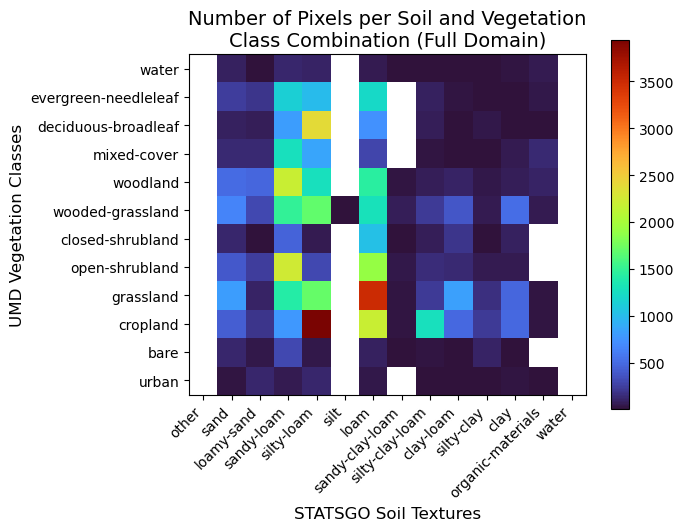
\includegraphics[width=.75\linewidth,draft=false]{figures/static_soil-veg-combos.png}
    \caption{Full-domain combination matrix of vegetation and soil classes}
    \label{static-combos}
\end{figure}

\begin{figure}[hp!]
    \centering
    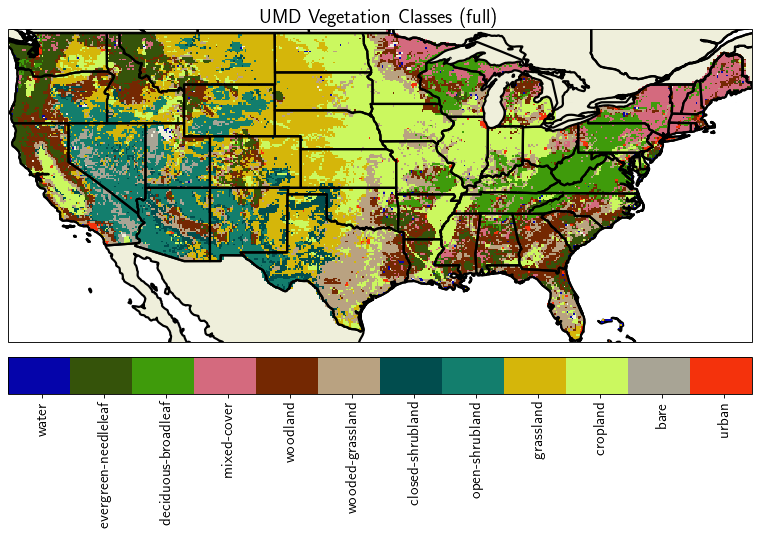
\includegraphics[width=.85\linewidth,draft=false]{figures/static_umd-veg-classes_full.png}
    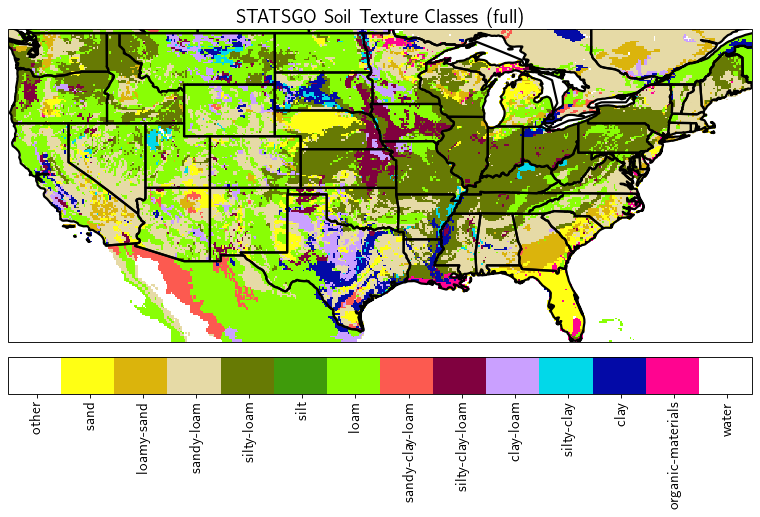
\includegraphics[width=.85\linewidth,draft=false]{figures/static_statsgo-soil-classes_full.png}
    \caption{Spatial distribution of vegetation and soil classes}
    \label{static-classes}
\end{figure}

\begin{figure}[hp!]
    \centering
    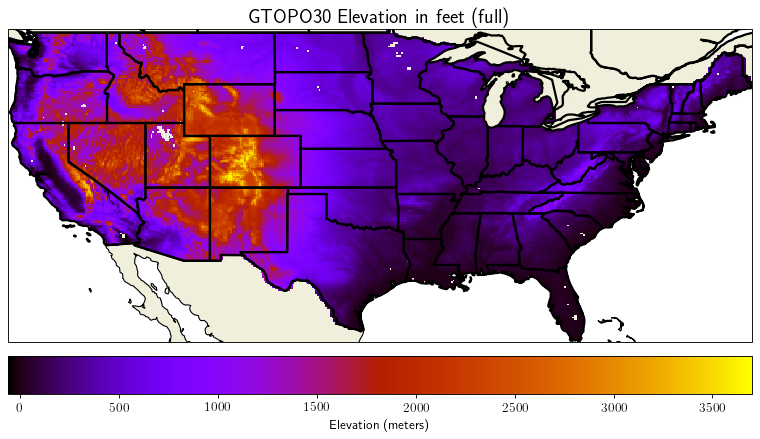
\includegraphics[width=.85\linewidth,draft=false]{figures/static_elev_full.png}
    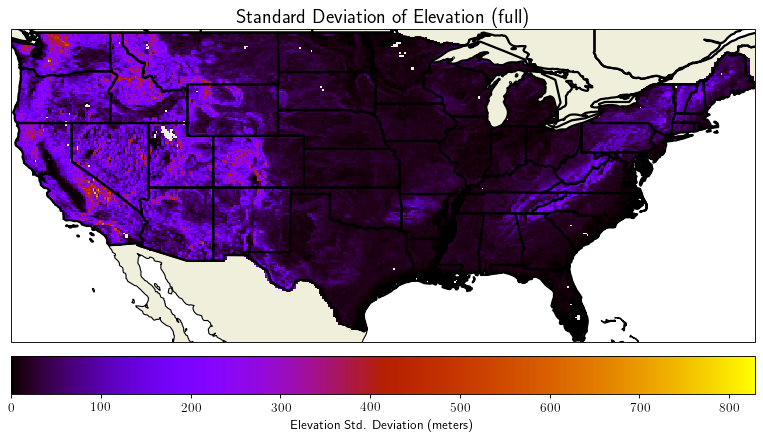
\includegraphics[width=.85\linewidth,draft=false]{figures/static_elev-stdev_full.png}
    \caption{Elevation and standard deviation of elevation on the CONUS domain}
    \label{static-elevation}
\end{figure}

One important aspect of the NLDAS-2/Noah-LSM datasets is the relationship between static and dynamic parameters, and the regional variance of both of these input types. Given any particular forcing time series, the subsequent land surface response is modulated by values for vegetation type, soil texture, slope, slope aspect, and a drainage parameter referred to as slope type, which are consistent per-pixel throughout the dataset. In this work, we will only train models informed by the first four. Slope and aspect were left out because within Noah-LSM they are only used within the snowpack parameterization \citep{barlage_noah_2010}, and snow is generally not a target variables for the models presented here. Furthermore, slope correlates strongly with the standard deviation of elevation. Slope type isn't well-documented in the model, and wasn't considered during training, but had a noticable effect on some of the results. In retrospect, these inputs may have increased the information available to the models for estimating the transference of water from snow melt to the soil layers, especially in mountainous regions like the Rocky Mountain and Sierra Nevada ranges. An evaluation of the impact of these parameters on model results is left for future work. Elevation parameters aren't directly utilized within Noah-LSM, but it is used to perform orographic regressions on pressure, temperature, humidity, and precipitation while resampling forcing data. Thus it is included as a training input because it could be useful as a predictor that indicates processes relevant to mountain snowpack dynamics.

As described in the background, the vegetation classes encode the properties of the canopy relevant to precipitation interception and land surface shading, the efficiency of plant transpiration at removing water from the soil, and the number of layers from which water is drawn (that is, the rooting depth). Since the vegetation parameter is discretely categorical within the Noah-LSM algorithm, we employ a special method of introducing them into the model called class embedding, which is elaborated upon in the next subsection.

\begin{table}[H]
    \centering
    \scriptsize
    \begin{tabular}{c|c|c|c|c|c|c }
Texture & \thead{Porosity \\ ($m^3/m^3$)} & \thead{Field Cap. \\ ($m^3/m^3$)} & \thead{Wilting Pt. \\ ($m^3/m^3$)} & \thead{B Param. \\ (dimless)} & \thead{Hydr. Cond. \\ ($mm/s$)}\\
\hline
Sand & 0.395 & 0.275 & 0.023 & 4.050 & 0.968 \\
Loamy Sand & 0.421 & 0.317 & 0.028 & 4.260 & 0.077 \\
Sandy Loam & 0.434 & 0.343 & 0.047 & 4.740 & 0.029 \\
Silty Loam & 0.476 & 0.389 & 0.084 & 5.330 & 0.015 \\
Silt & 0.476 & 0.389 & 0.084 & 5.330 & 0.015 \\
Loam & 0.439 & 0.356 & 0.066 & 5.250 & 0.019 \\
Sandy Clay Loam & 0.404 & 0.337 & 0.069 & 6.770 & 0.024 \\
Silty Clay Loam & 0.464 & 0.406 & 0.120 & 8.720 & 0.011 \\
Clay Loam & 0.465 & 0.403 & 0.103 & 8.170 & 0.013 \\
Silty Clay & 0.468 & 0.420 & 0.126 & 10.390 & 0.007 \\
Clay & 0.457 & 0.416 & 0.135 & 11.550 & 0.005 \\
Organic & 0.464 & 0.377 & 0.069 & 5.250 & 0.019 \\
\end{tabular}
    \caption{Soil hydraulic properties associated with each texture class from \citep{cosby_statistical_1984}.}
    \label{soil-texture-table}
\end{table}

%The soil texture class corresponds to a variety of hydraulic properties identified by \citep{cosby_statistical_1984}, which include field capacity, hydraulic conductivity, porosity, wilting point, matric potential, and Skempton's pore water pressure (``B'' parameter). These describe physical characteristics of the soil-water system including the rate of downward percolation of water, the efficiency and limits of plant water uptake, the speed of infiltration, and the total amount of water that soil can contain per unit volume. The basic observable feature of soil that determines all of the hydraulic properties is the size distribution of its constituent particles, which is often articulated as the mass fraction of sand, silt, and clay components within the soil. In the interest of providing the models with real-valued inputs having relatively low dimensionality, these three texture components will serve as the representation of soil texture for the ANNs trained here.

In Noah-LSM, each pixel is assumed to have a vertically uniform soil texture throughout the column. The texture associated with each pixel is based on the surface of the 11-layer spatial soil dataset developed by \citep{miller_conterminous_1998}, as pictured in Figure \ref{static-classes}. Each texture category is mapped to a variety of hydraulic properties mainly based on measurements taken by \citep{cosby_statistical_1984}. These parameters include field capacity, hydraulic conductivity, porosity, wilting point, matric potential, and the exponential``B'' parameter of the soil water retention curve. The basic observable feature of soil that determines all of the hydraulic properties in the scheme used by the model is the size distribution of its constituent particles, which is often articulated as the mass fraction of sand, silt, and clay components within the soil. In the interest of providing the models with real-valued inputs having relatively low dimensionality, these three texture components will serve as the representation of soil texture for the ANNs trained here.

Table \ref{soil-texture-table} lists each of the soil textures alongside their hydraulic parameters. We will now briefly discuss how each parameter affects soil dynamics based on \citep{dingman_physical_2014}. The porosity is the ratio of a volume of soil that is not occupied by solids like minerals and organic compounds, which determines the limit of the material amount of water that the soil can contain at saturation. Counterintuitively, coarse soils like sand have lower porosity than clay-dominant soils because the grain shapes associated with sand are packed more efficiently than clay, and as such sand can have a lower maximum water capacity per unit volume. Ignoring the influence of evapotranspiration, gravity will cause water to gradually drain downward through unsaturated soil at an exponentially decreasing rate consistent with the Richards Equation. Under these circumstances, the field capacity of a soil is the volume fraction of soil water at which the rate of drainage is negligible. As such, when the soil water content is below the field capacity, the only processes that further decrease the water content are evapotranspiration and capillary diffusion to a drier adjacent soil layer. The enhanced adhesive forces associated with finer-grained soils like clay grant them a field capacity that is much closer to their porosity than a coarser soil like sand, so for finer soils evapotranspiration and diffusion will dominate the dynamics except when the soil is close to saturation. The wilting point is defined in terms of volume fraction of soil water based on the suction pressure plants are able to exert on the soil in order to remove water, which is typically assumed to be $-1,470\,kPa$. Once the soil reaches the wilting point, the process of plant transpiration ceases, and the only process that may still diminish water in the soil layer is diffusion.

The hydraulic conductivity of a soil describes the rate at which water can move through the soil against the friction of the soil matrix. Soils with large pore sizes like sand have a dramatically higher hydraulic conductivity than finer soils, and as such can transmit infiltrated water much more rapidly to lower layers. The values given in Table \ref{soil-texture-table} refer to the hydraulic conductivity at saturation, however in practice the hydraulic conductivity has a highly nonlinear relationship with the soil water content such that it decreases following an exponential curve that must be empirically determined. This relationship is defined in terms of the B parameter, which is inversely proportional to the mean pore size of each soil texture. While the hydraulic conductivity of a soil at saturation is a constant, the hydraulic conductivity of fine-grained soils with a large B parameter decreases much faster as the soil dries compared to coarser soils, which maintain relatively large hydraulic conductivities at mid or low-range water content. Soil water diffusion is a separate important term in the Richards equation which governs the movement of water across a moisture gradient between layers as a consequence of capillary action, which enables the upward percolation of water, and moisture exchange between soil layers when the water content is below the field capacity. Diffusion is also defined in terms of an exponential relationship with the B parameter, described a nonlinear differential equation without an analytic solution. Coarser soils tend to have higher diffusivities close to saturation that peak just below saturation, while finer soils have lower diffusivities that more rapidly diminish as the soil dries.

The interplay between plant water uptake and soil water dynamics as governed by the static inputs represents a considerable source of complexity within Noah-LSM. Furthermore, as Figure \ref{static-combos} demonstrates, the distribution of combinations of soil and vegetation categories is extremely non-uniform, which makes it more difficult for ANNs to learn solutions that are general. Figure \ref{static-classes} shows the geographic locations of vegetation and soil classes. The most common class combination is silty-loam soil types juxtaposed with cropland, with 3,945 members found dominantly in the Midwest and lower Mississippi river basin, with some contribution from the Columbia Plateau in Washington and Eastern Nebraska. Next most common are the 3,490 pixels in loamy grasslands, which are distributed widely throughout the West US including the high plains, Western Texas and New Mexico,  Utah, and Idaho. The remaining combinations all have fewer than 2,500 members within the domain. Sand and clay dominated soils form the upper and lower extremes of soil particle size, respectively, and thus have rather different soil water characteristics. The sandiest soils are found in Southern Coastal Plains, Michigan, Texas, the Nebraska Sandhills, and the desert Southwest. Clay soils are relatively rare compared to silty and sandy soils, and considerably more spatially heterogeneous. They are mainly found in tight groupings around Central Texas, the Mississippi Alluvial Plain, Eerie Lake Plains, and the Missouri River Basin in South Dakota. Despite their infrequency, clay soils span the full range of surface classes.

\begin{figure}[h!]
    \centering
    %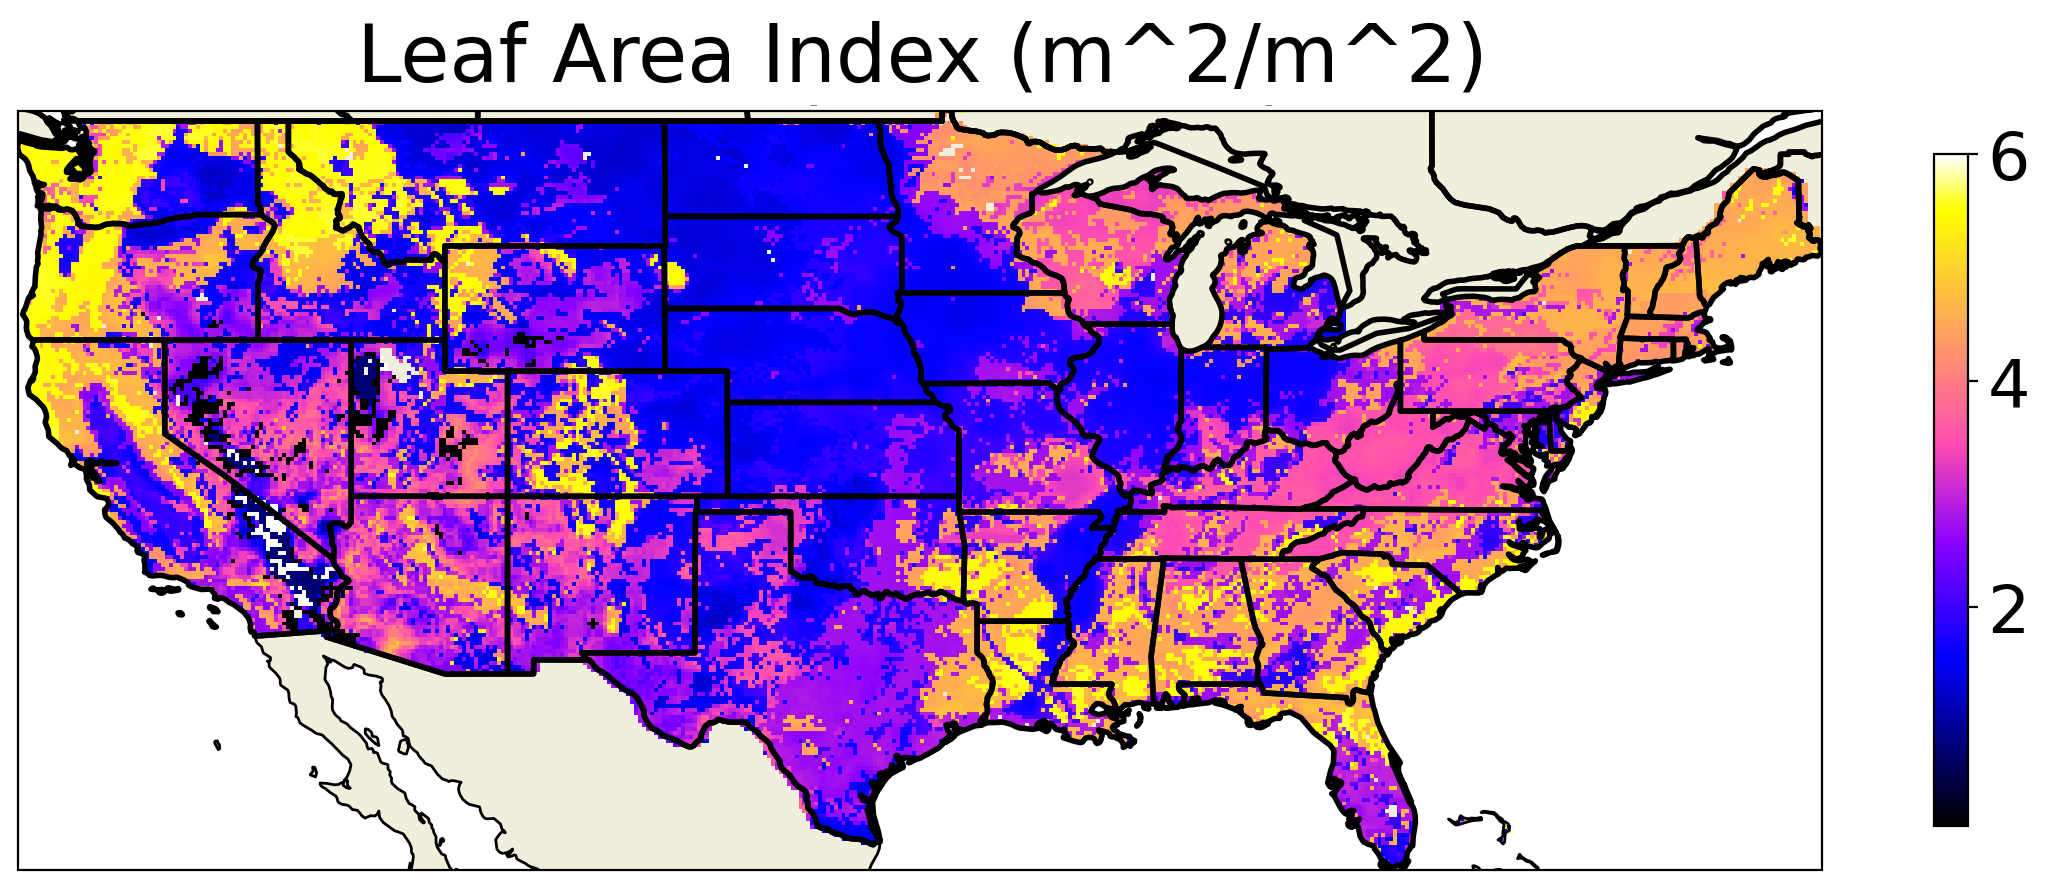
\includegraphics[width=.48\linewidth,draft=false]{figures/thesis-gridstats/gridstat-bulk_lai_2012-1_2023-12_y000-195_x000-462_mean.png}

    %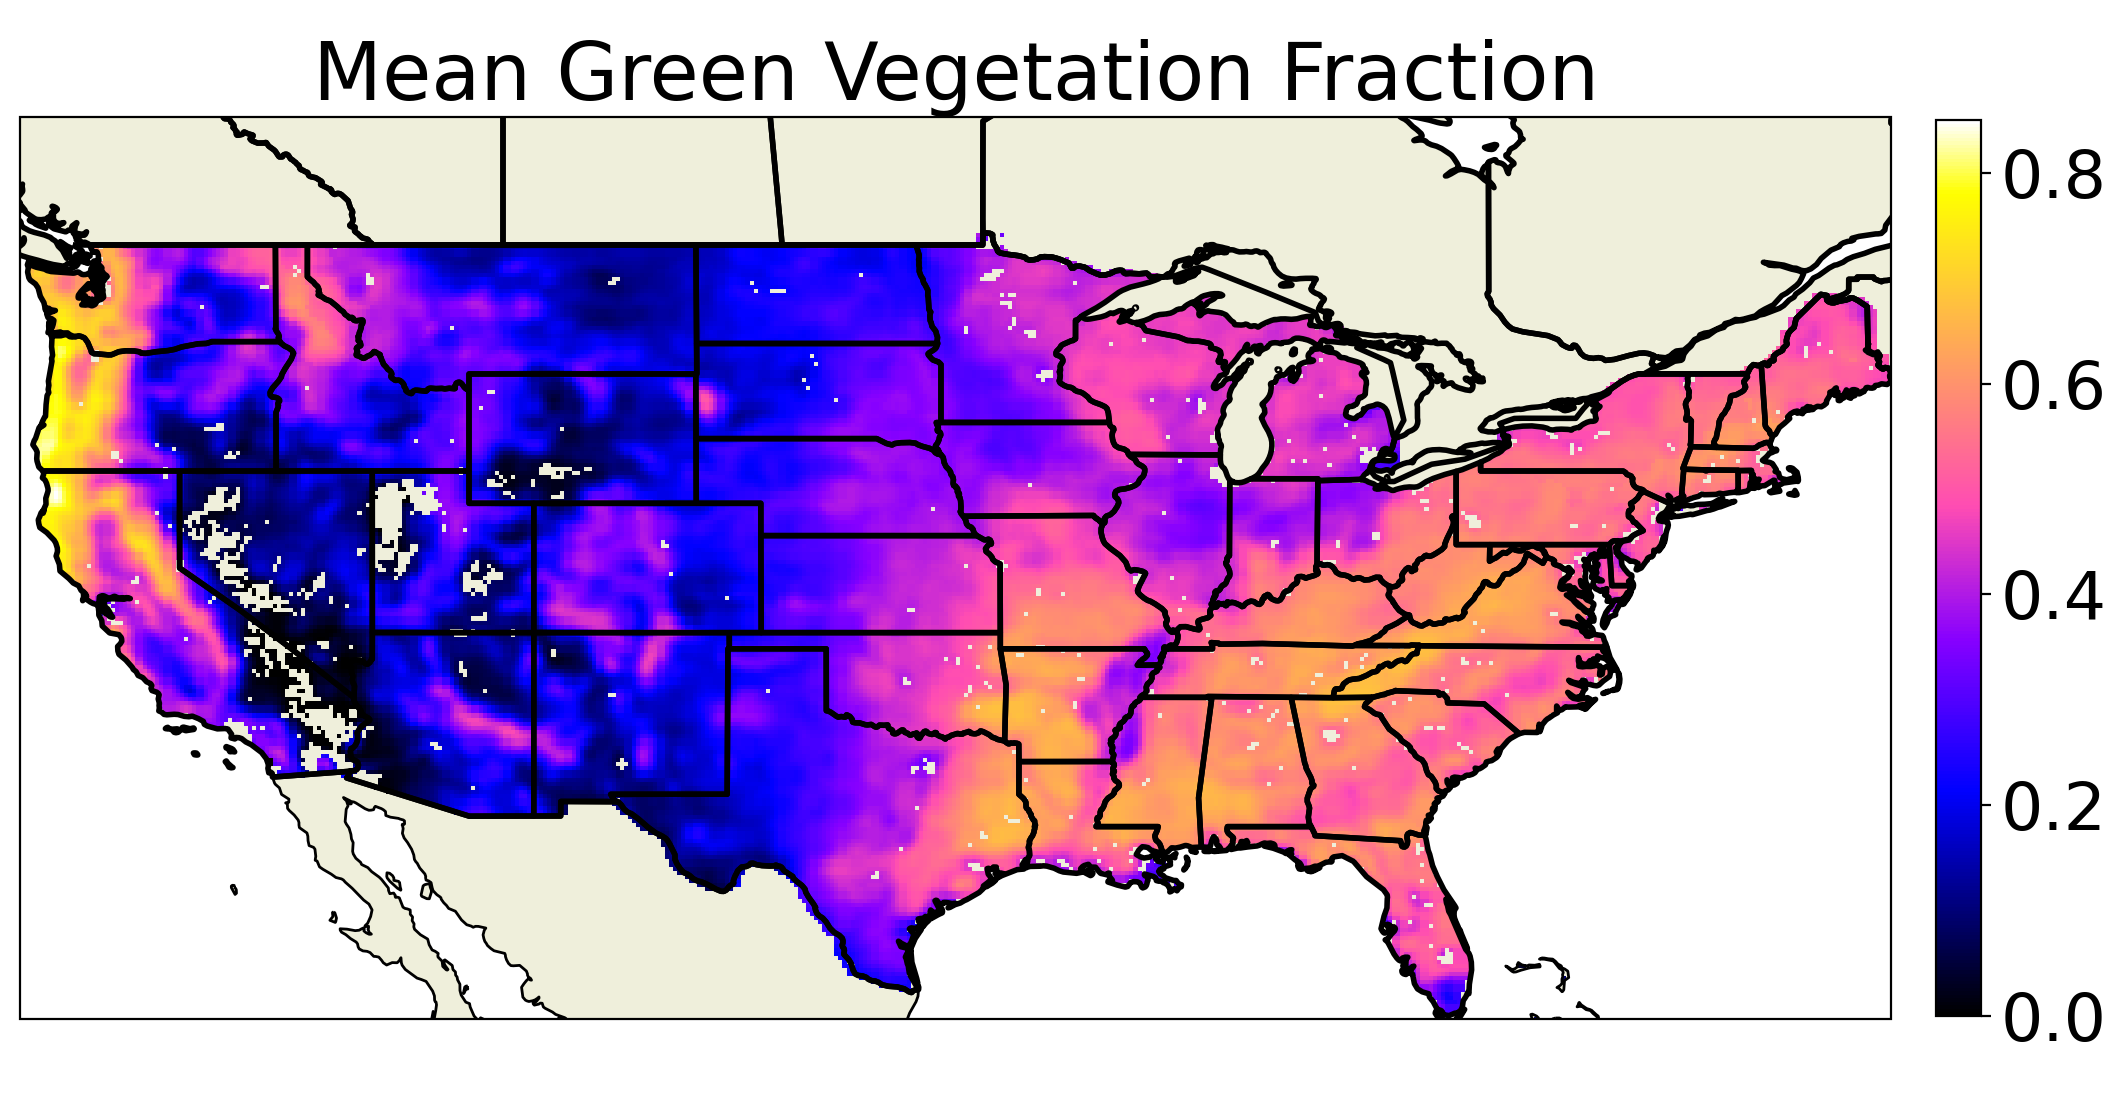
\includegraphics[width=.48\linewidth,draft=false]{figures/thesis-gridstats/gridstat-bulk_veg_2012-1_2023-12_y000-195_x000-462_mean.png}
    %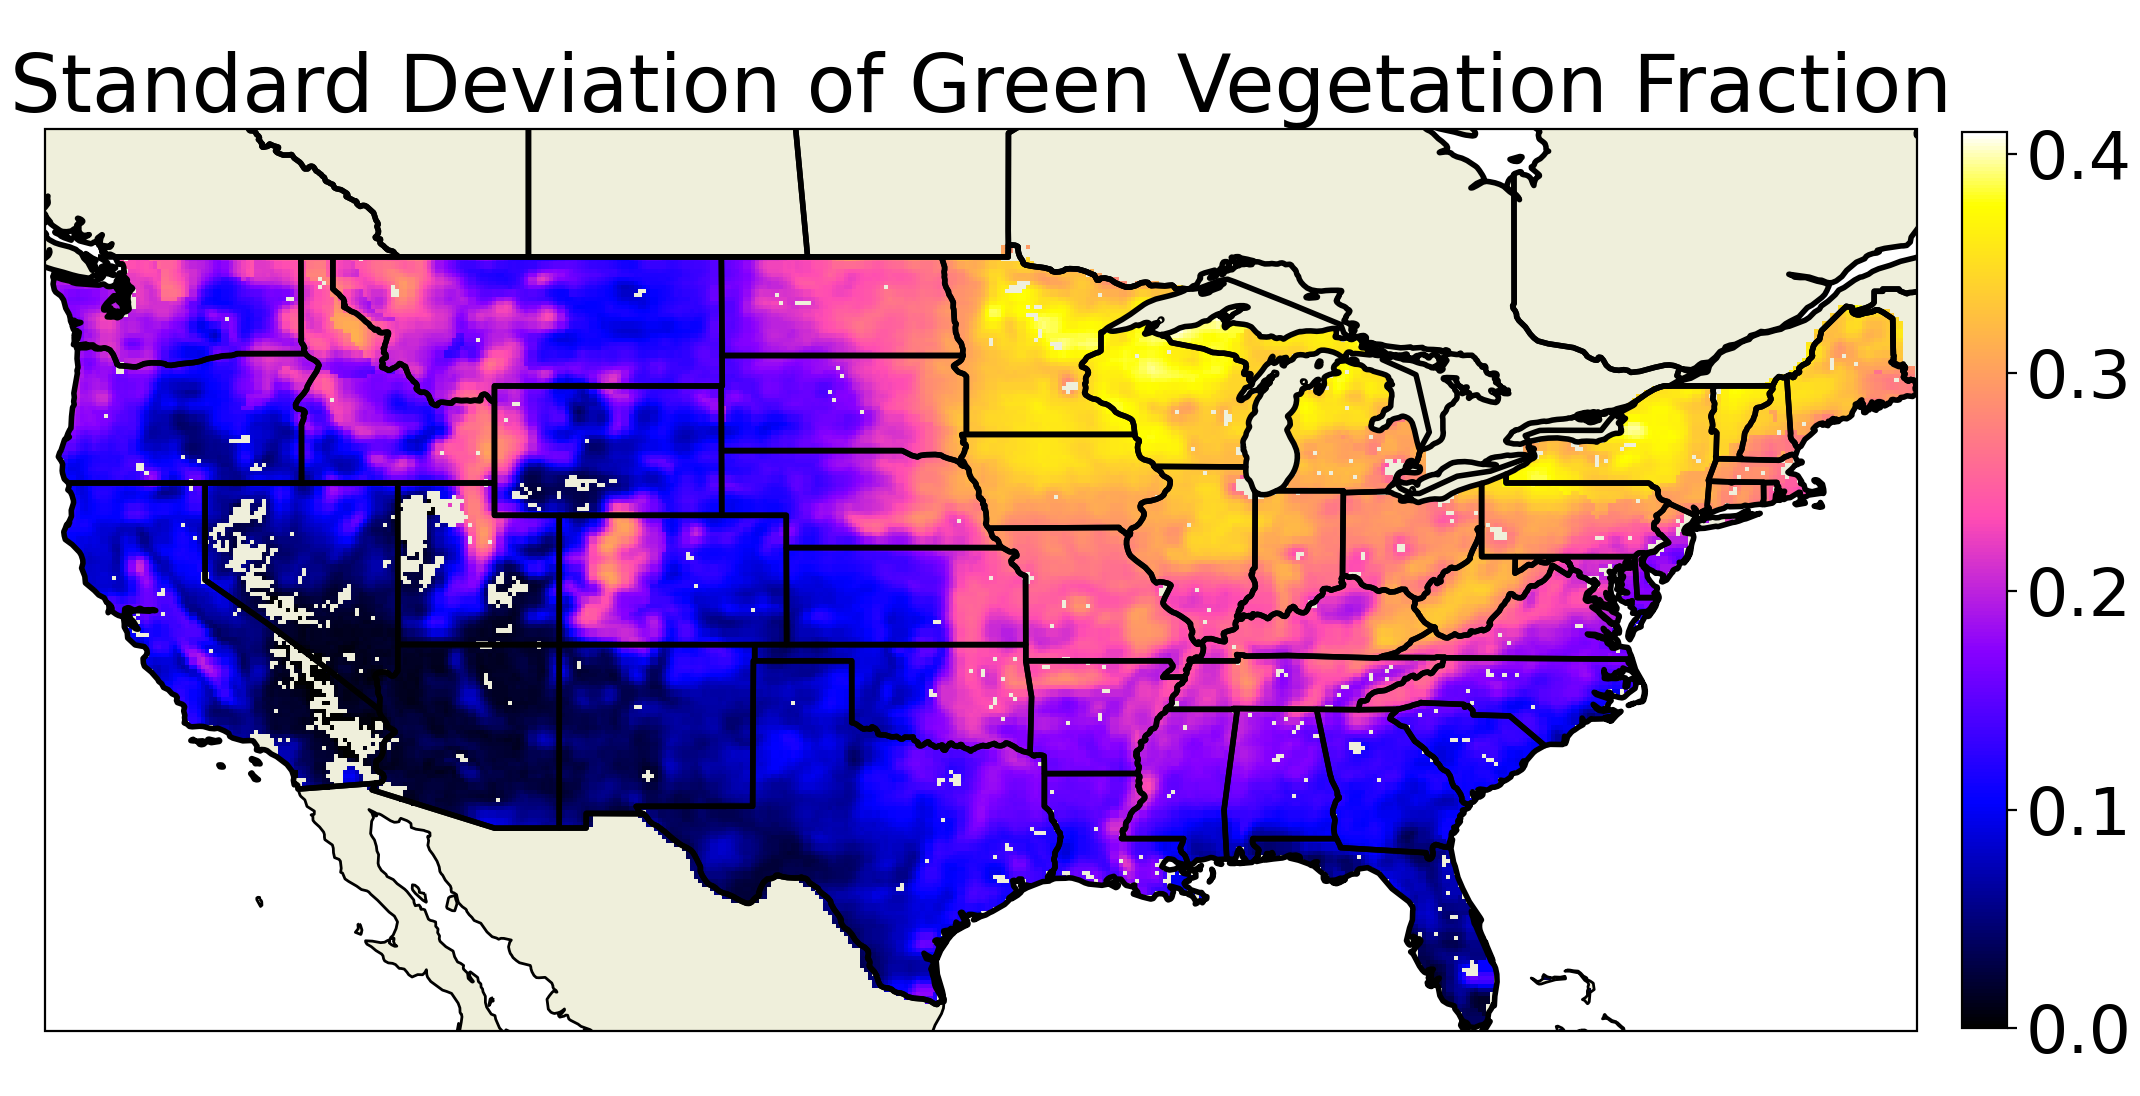
\includegraphics[width=.48\linewidth,draft=false]{figures/thesis-gridstats/gridstat-bulk_veg_2012-1_2023-12_y000-195_x000-462_stdev.png}
    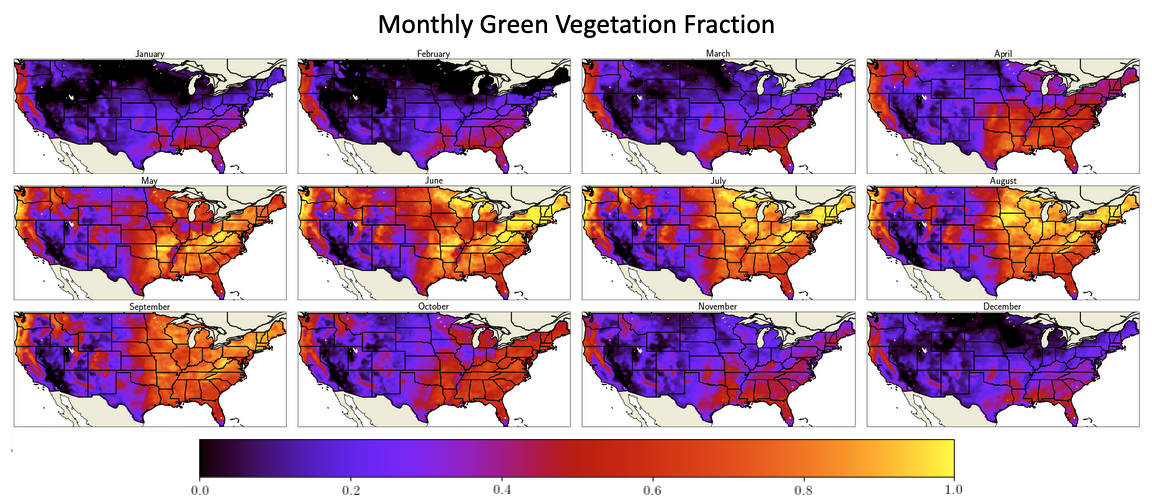
\includegraphics[width=.98\linewidth,draft=false]{figures/gvf/gvf_mosaic.png}

    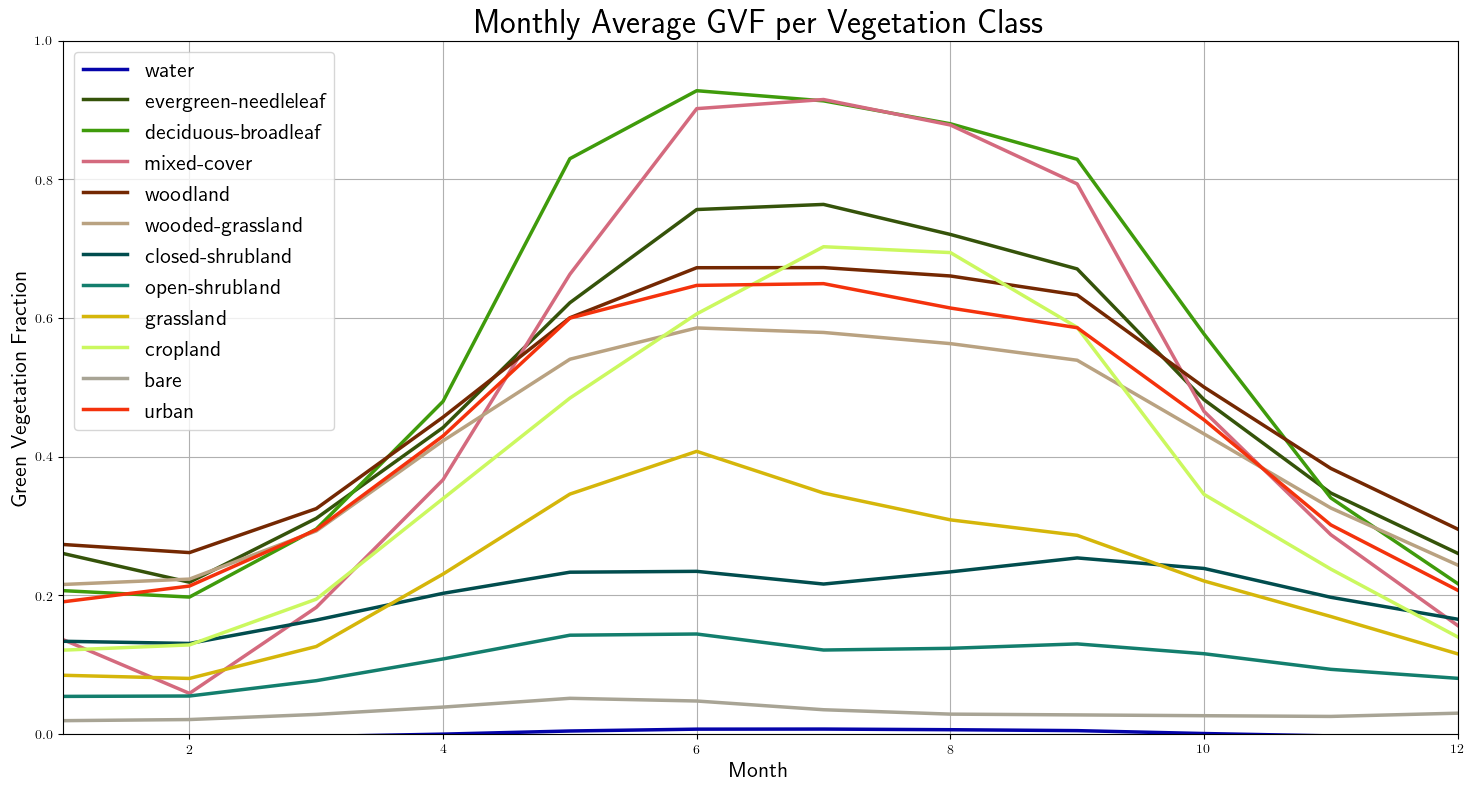
\includegraphics[width=.48\linewidth,draft=false]{figures/gvf/gvf_monthly_stats.png}
    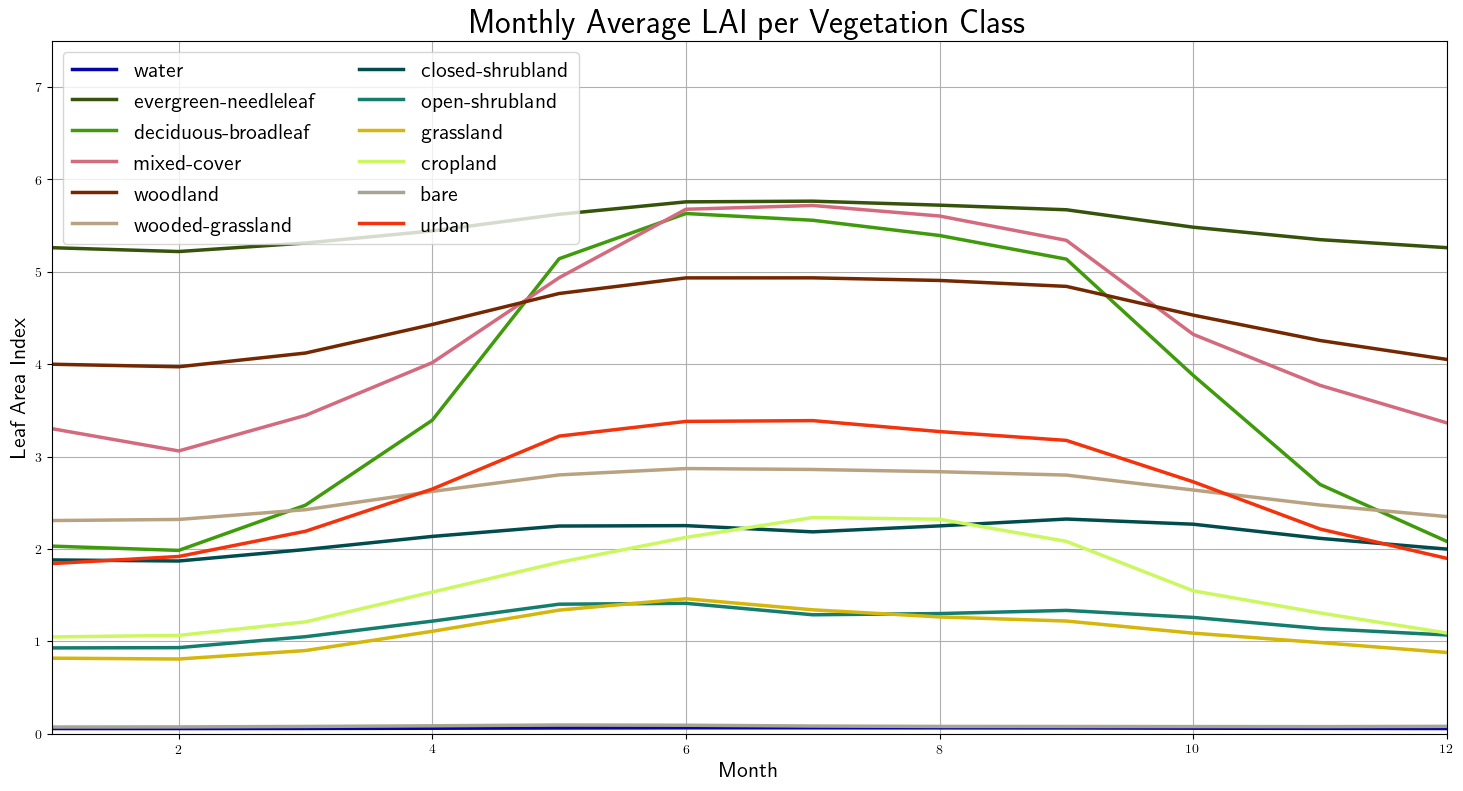
\includegraphics[width=.48\linewidth,draft=false]{figures/gvf/lai_monthly_stats.png}
    \caption{Monthly average green vegetation fraction (top), and monthly time series of GVF (bottom left) and LAI (bottom right) per vegetation class.}
    \label{gs-vegetation}
\end{figure}

%Although they vary smoothly on an hourly basis, the LAI and GVF parameters are similar to static parameters in that they cycle consistently per-pixel on an annual basis (rather than dynamically changing based on variable atmospheric conditions), and modulate the soil water dynamics via through their effect on the vegetation parameterization. As Figure \ref{gs-vegetation} indicates, the densest annual-averaged canopy cover corresponds to evergreen needleleaf surface types, and there is almost no canopy over croplands and grasslands of the Midwest, California Valley, and the Great Plains. The greenest satellite-derived vegetation covers the West Coast and Sierra ranges, followed by the South and Northeast. The standard deviation of GVF indicates the regions of most significant seasonal variability, which corresponds to deciduous-dominant locales.

Although they vary smoothly on an hourly basis, the LAI and GVF parameters are similar to static parameters in that they cycle consistently per-pixel on an annual basis (rather than dynamically changing based on variable atmospheric conditions), and modulate the soil water dynamics via through their effect on the vegetation parameterization. Figure \ref{gs-vegetation} displays the monthly GVF averages retrieved by \citep{gutman_derivation_1998}, which have a substantial influence on the magnitude of plant transpiration. As defined in \citep{wei_improvement_2011}, the GVF directly scales the plant transpiration as a multiplicative coefficient, and also modulates the LAI between a minimum and maximum value that are uniquely specified for each surface category.

\begin{figure}[h!]
    \centering
    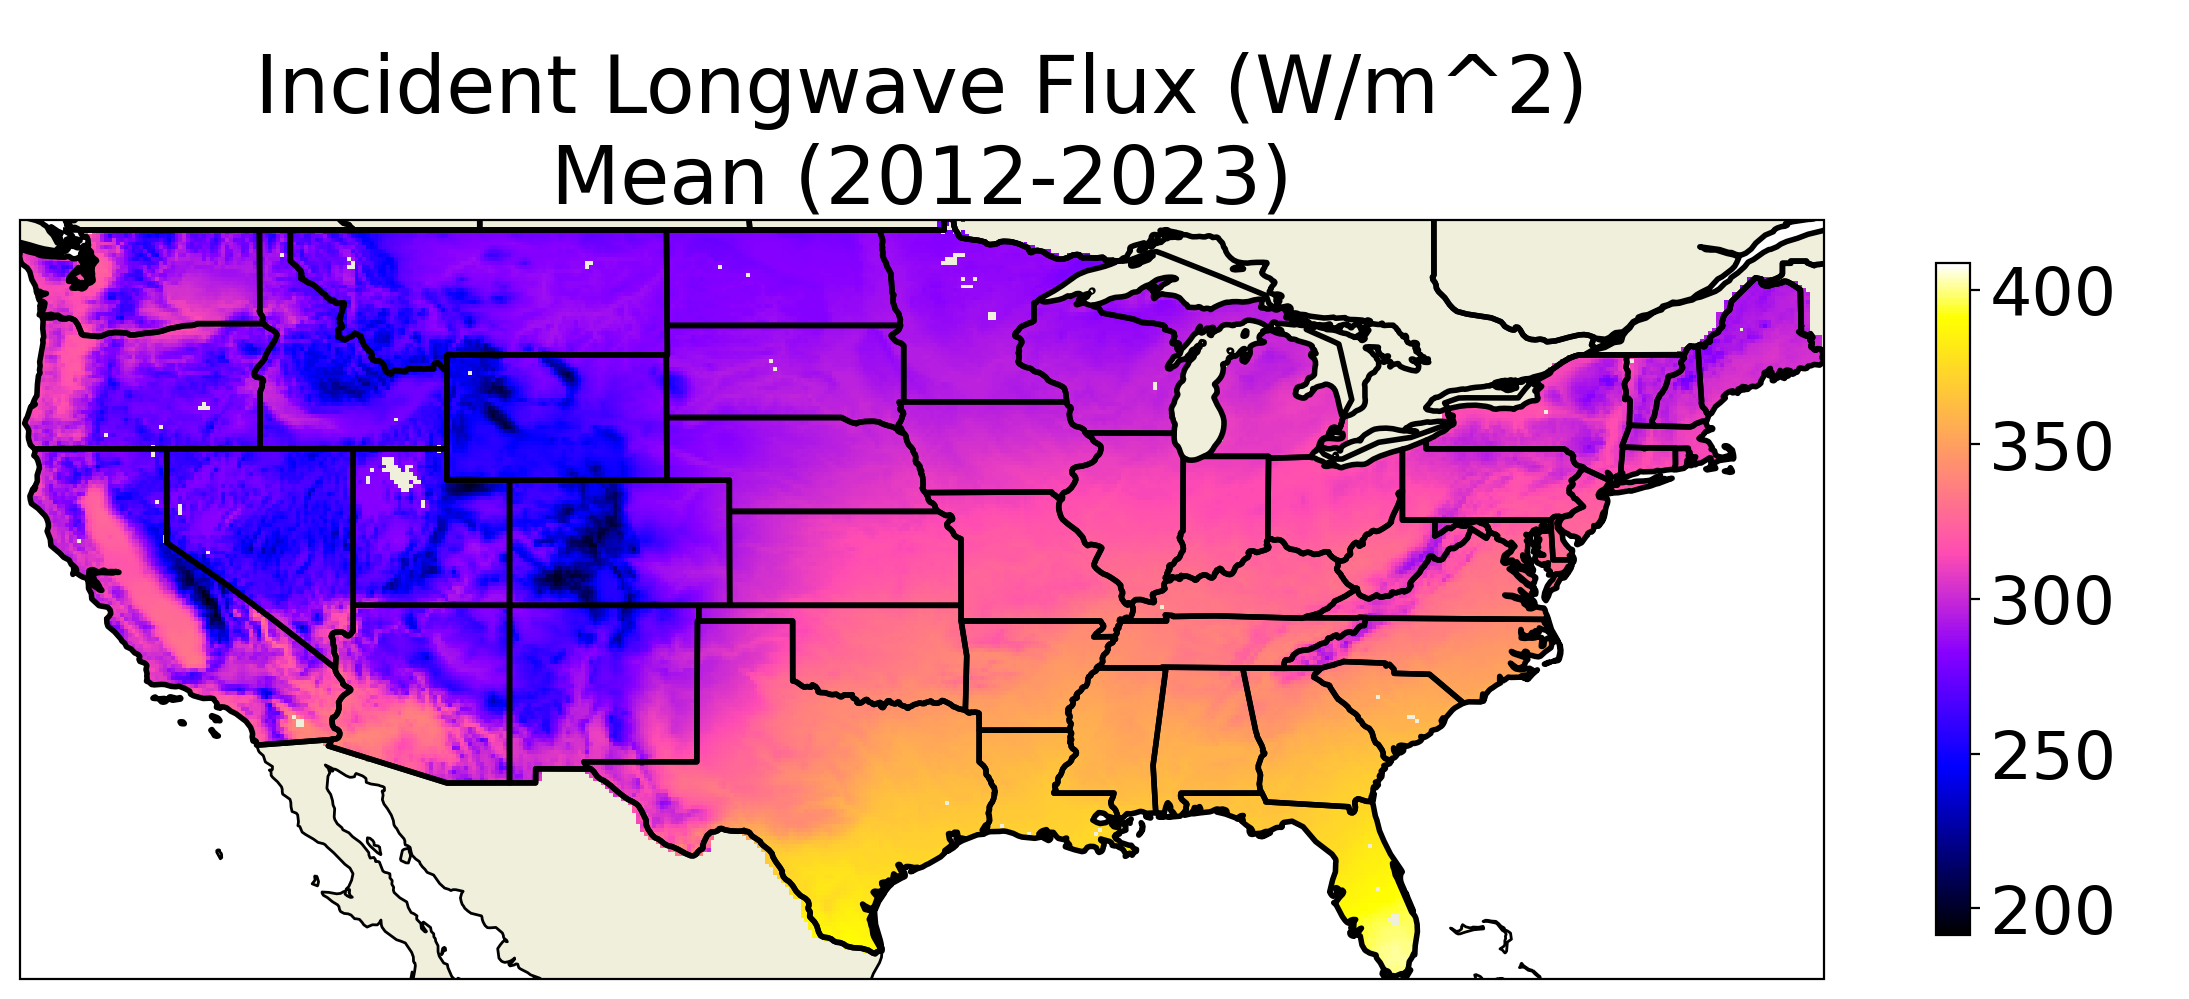
\includegraphics[width=.48\linewidth,draft=false]{figures/thesis-gridstats/gridstat-bulk_dlwrf_2012-1_2023-12_y000-195_x000-462_mean.png}
    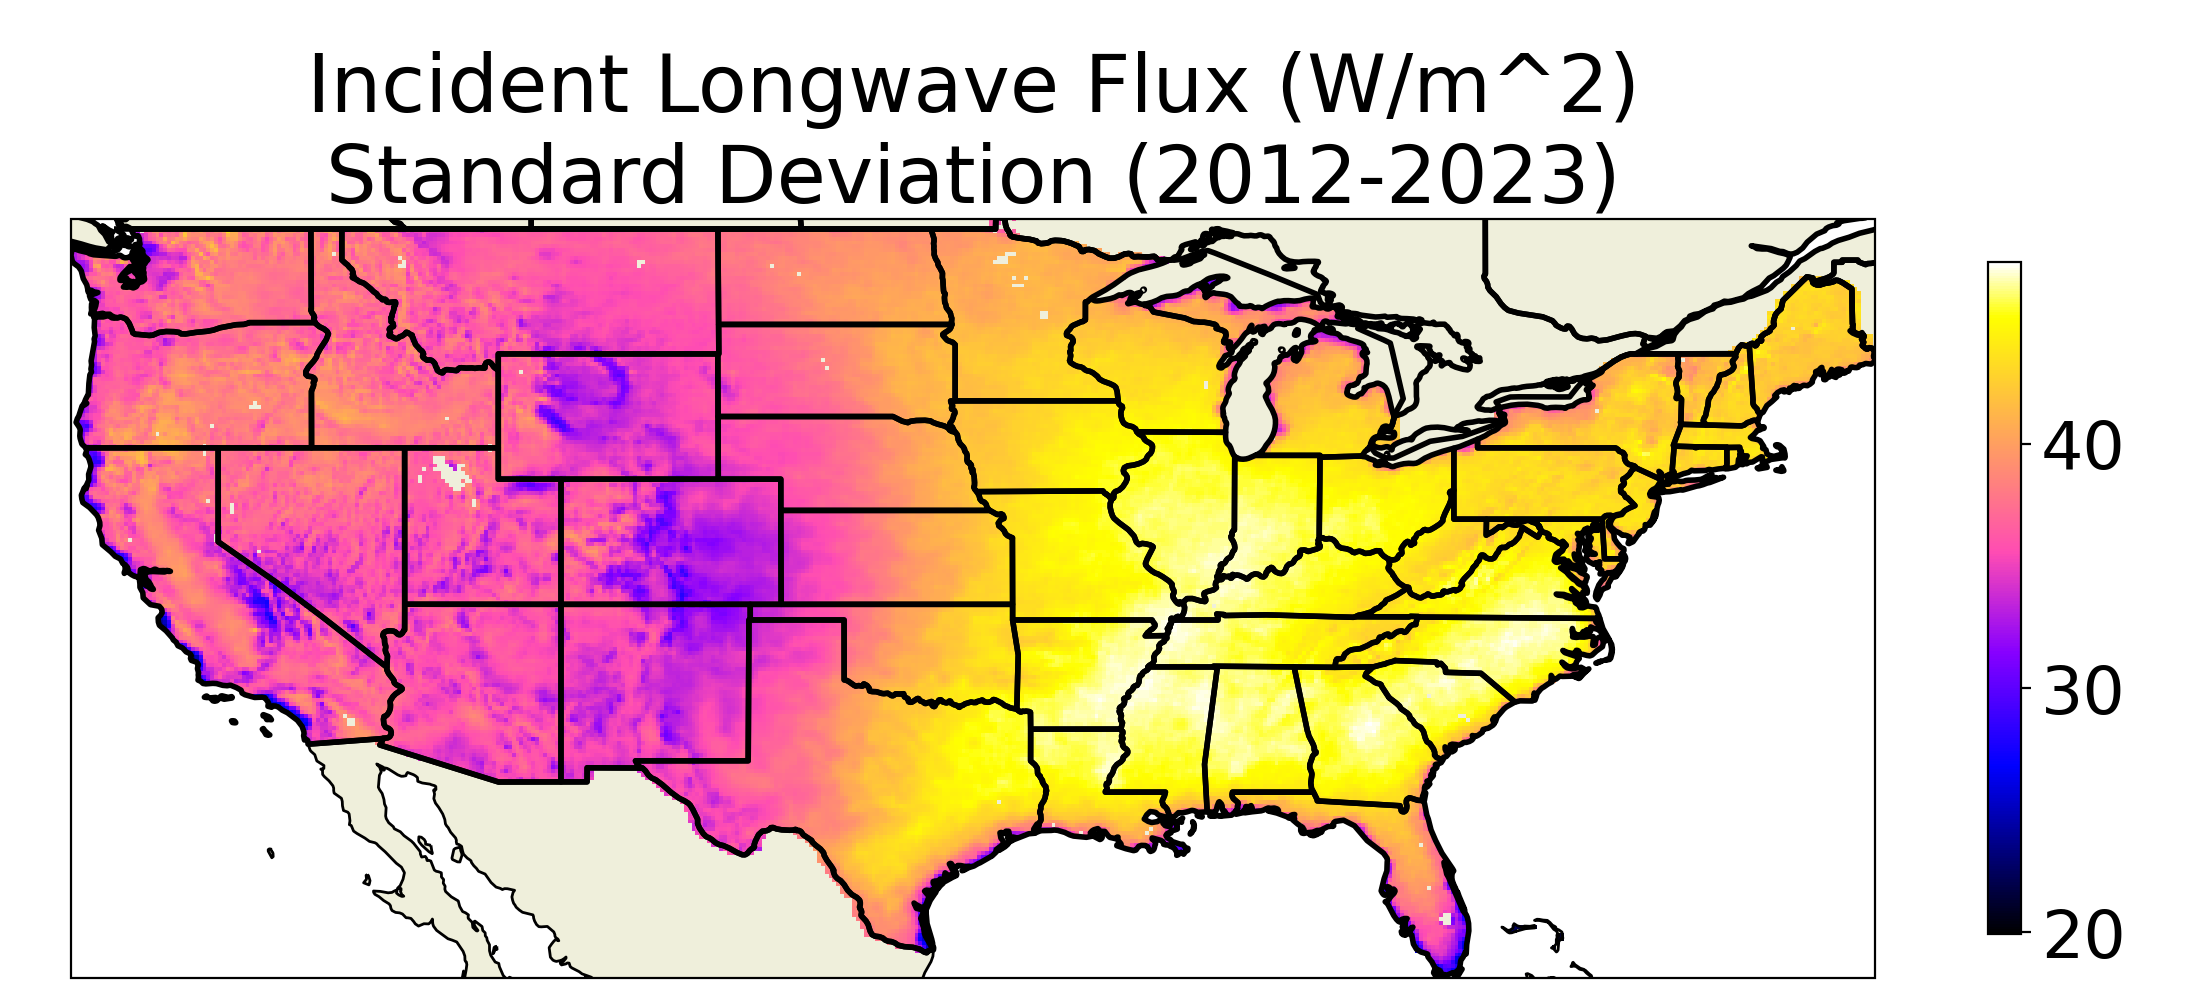
\includegraphics[width=.48\linewidth,draft=false]{figures/thesis-gridstats/gridstat-bulk_dlwrf_2012-1_2023-12_y000-195_x000-462_stdev.png}

    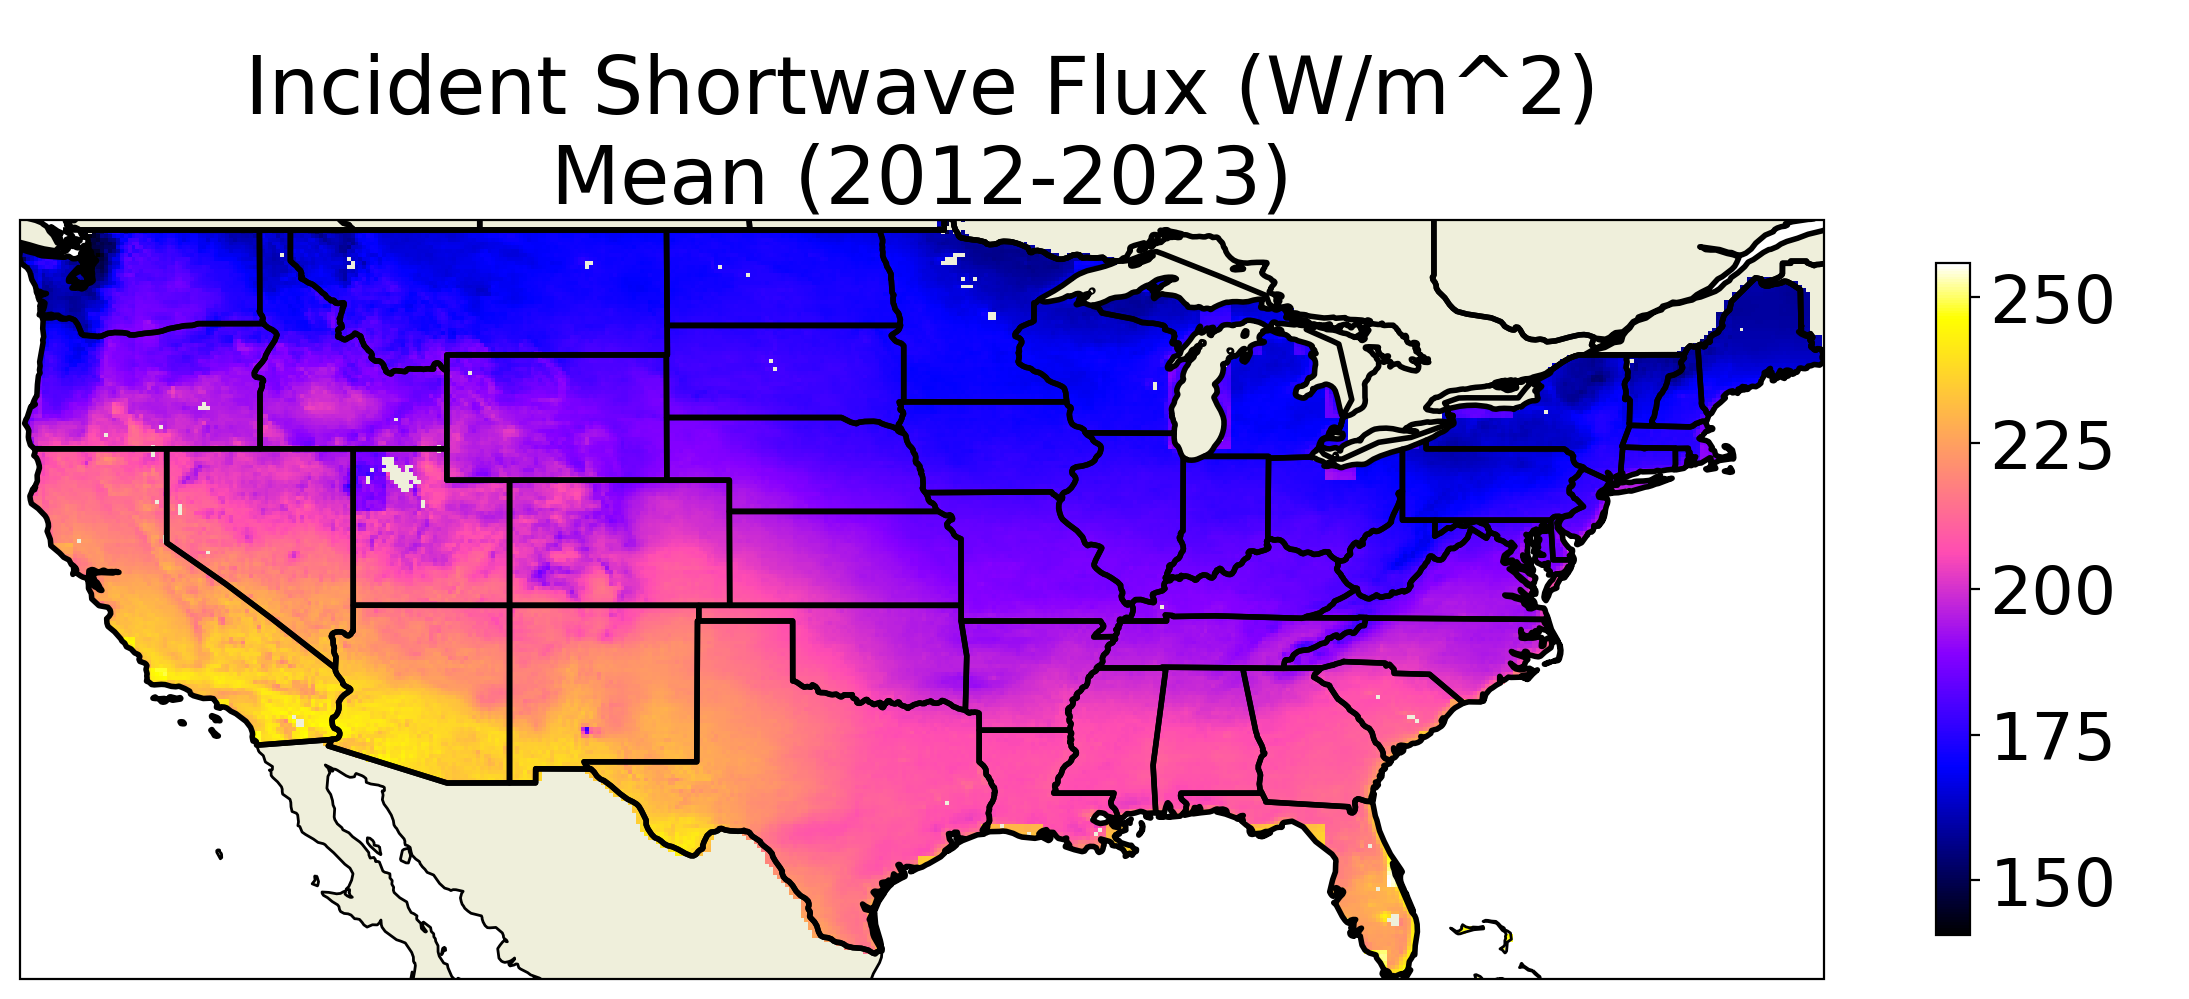
\includegraphics[width=.48\linewidth,draft=false]{figures/thesis-gridstats/gridstat-bulk_dswrf_2012-1_2023-12_y000-195_x000-462_mean.png}
    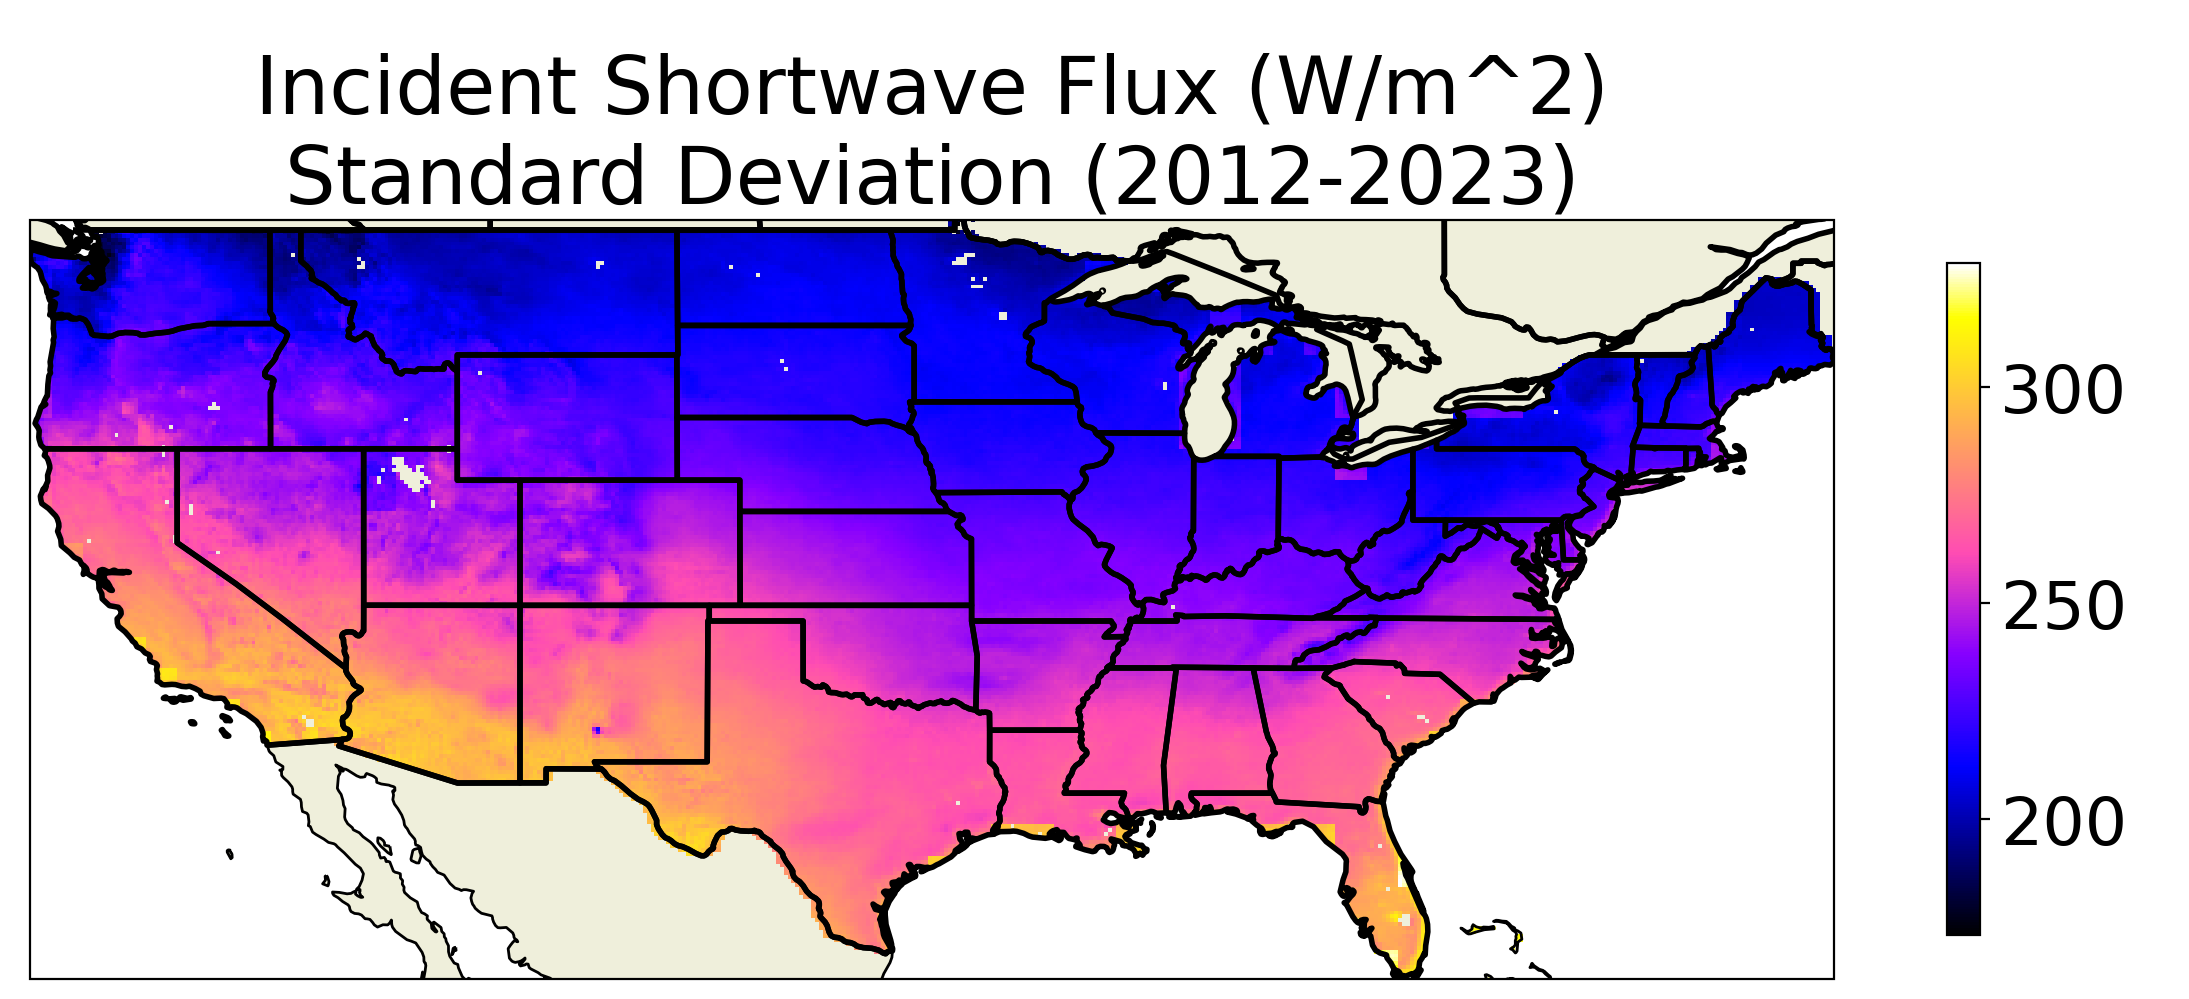
\includegraphics[width=.48\linewidth,draft=false]{figures/thesis-gridstats/gridstat-bulk_dswrf_2012-1_2023-12_y000-195_x000-462_stdev.png}
    \caption{Gridded mean and standard deviation of radiative forcings (2012-2023)}
    \label{gs-radiative}
\end{figure}

In addition to the substantial regional variability of the static parameterization of Noah-LSM, there are considerable regional and seasonal differences in the NLDAS-2 atmospheric forcing time series. Figure \ref{gs-radiative} shows the mean and standard deviation of radiative features over the full spatial and temporal domain, which demonstrates the distribution of annually-averaged downwelling radiation. Feedback from terrestrial emissions mean that longwave radiation is highest in regions that are generally cloudier, have warmer land surface temperatures, and are lower in elevation. The shortwave flux is highest at lower latitudes due to Earth's axial tilt, and in arid regions where there are fewer clouds.

\begin{figure}[hp!]
    \centering
    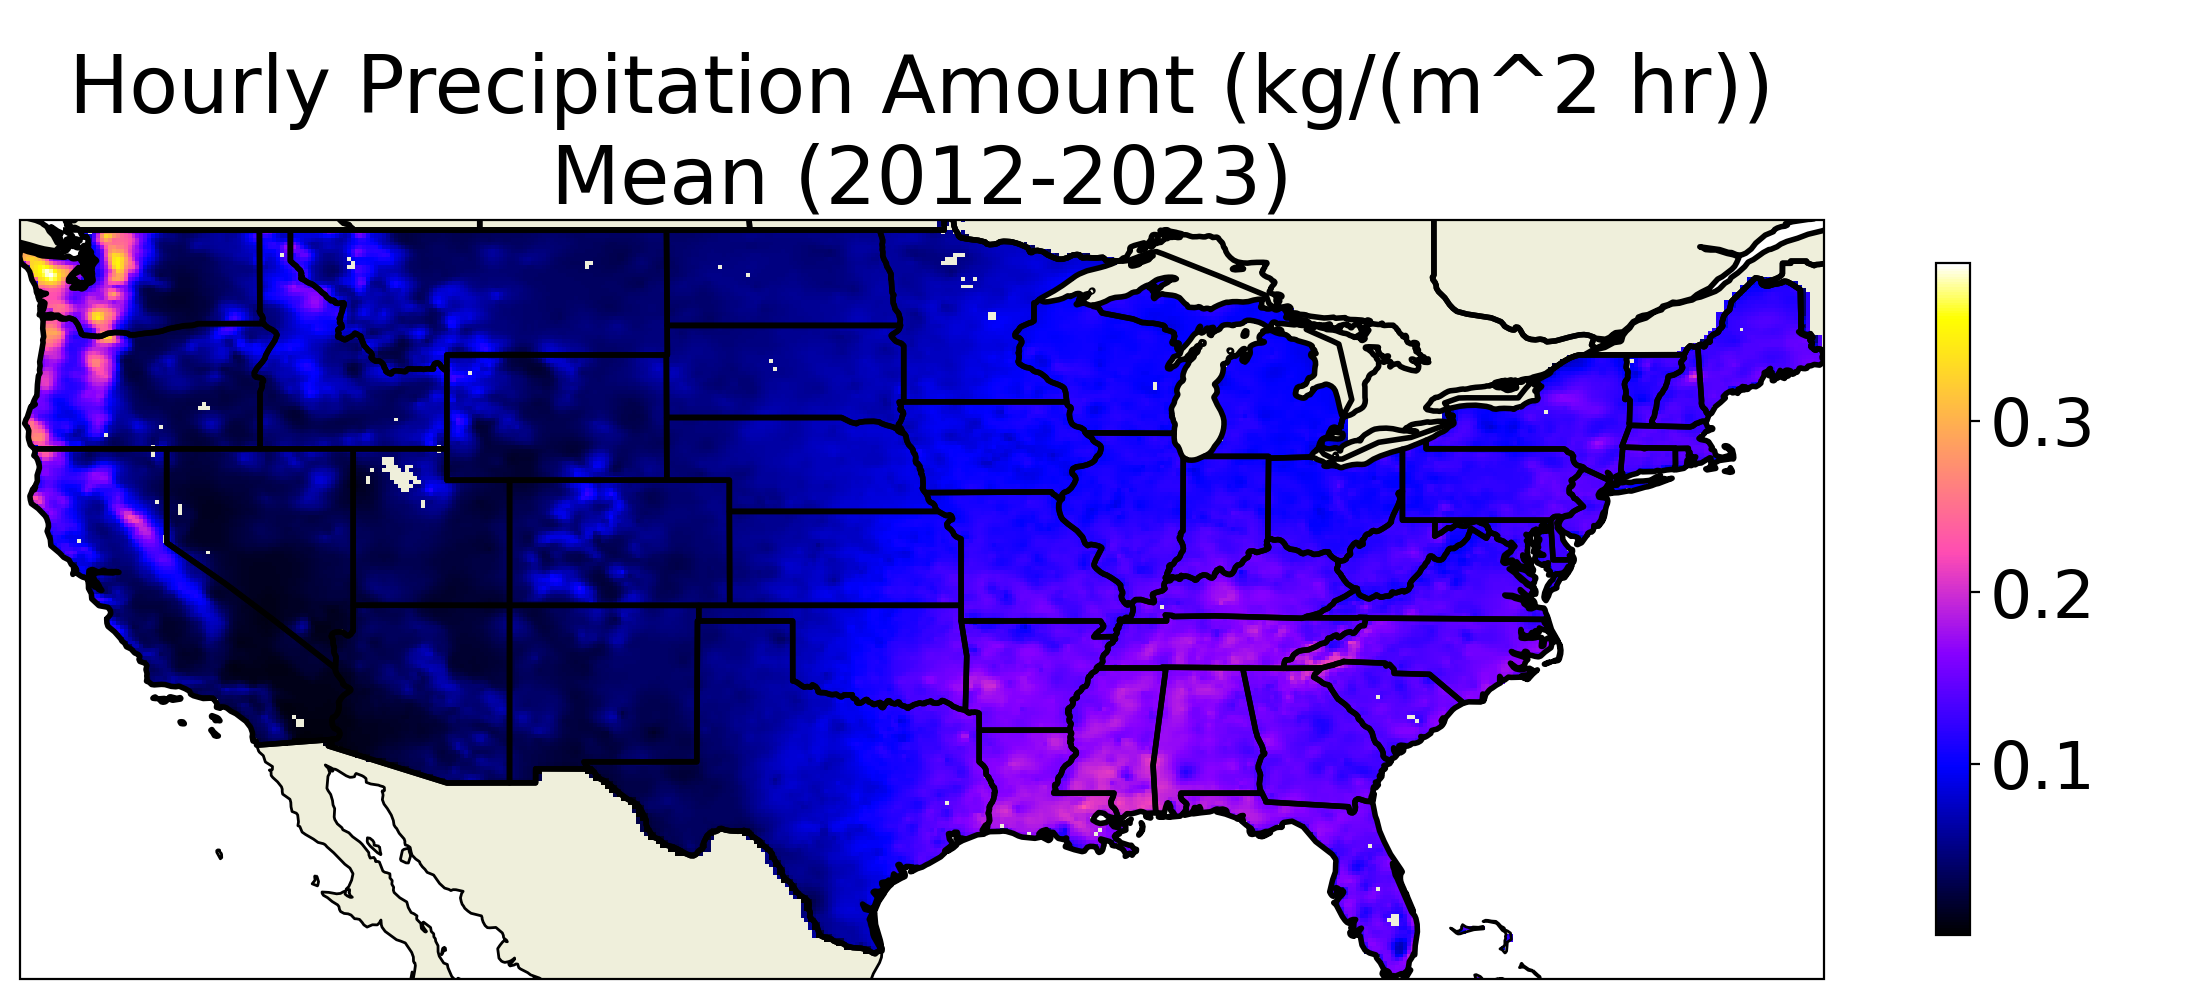
\includegraphics[width=.48\linewidth]{figures/thesis-gridstats/gridstat-bulk_apcp_2012-1_2023-12_y000-195_x000-462_mean.png}
    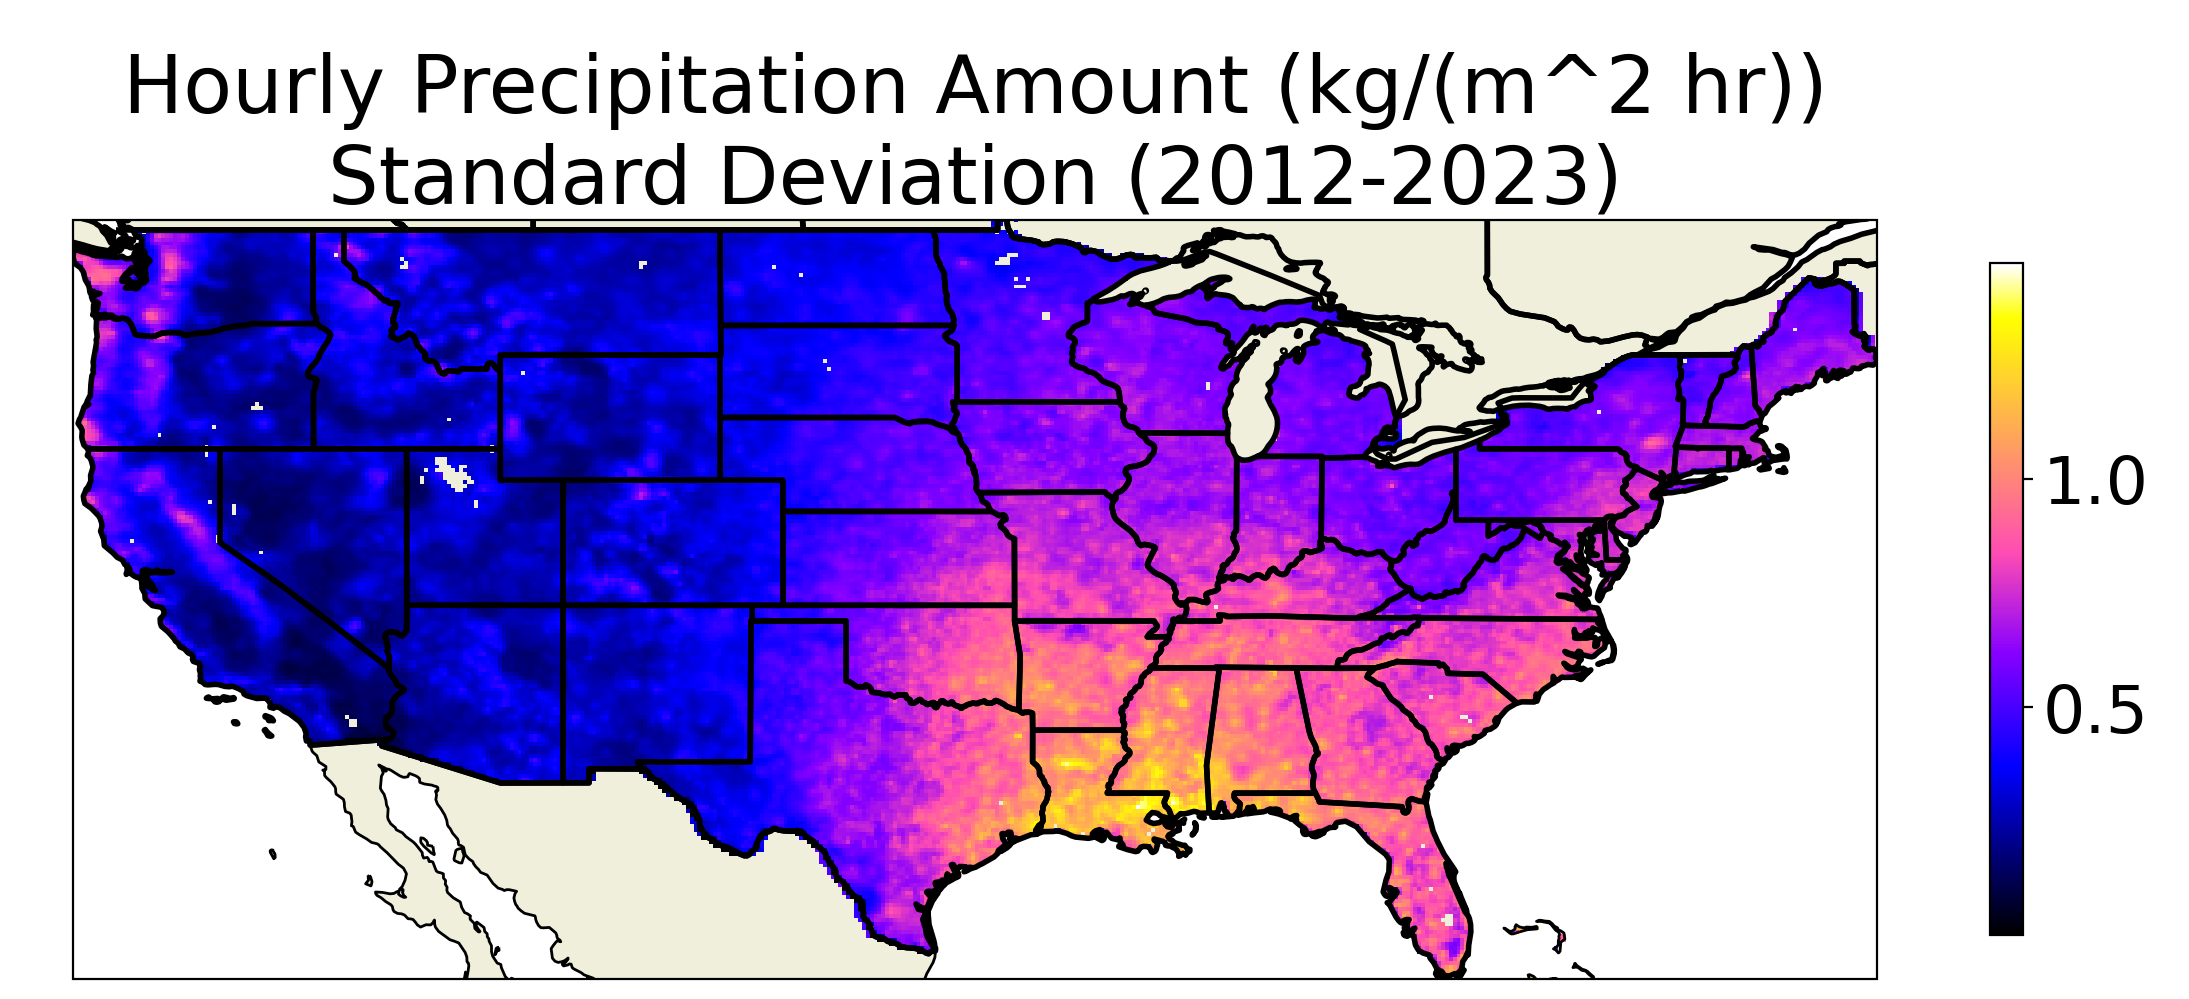
\includegraphics[width=.48\linewidth]{figures/thesis-gridstats/gridstat-bulk_apcp_2012-1_2023-12_y000-195_x000-462_stdev.png}

    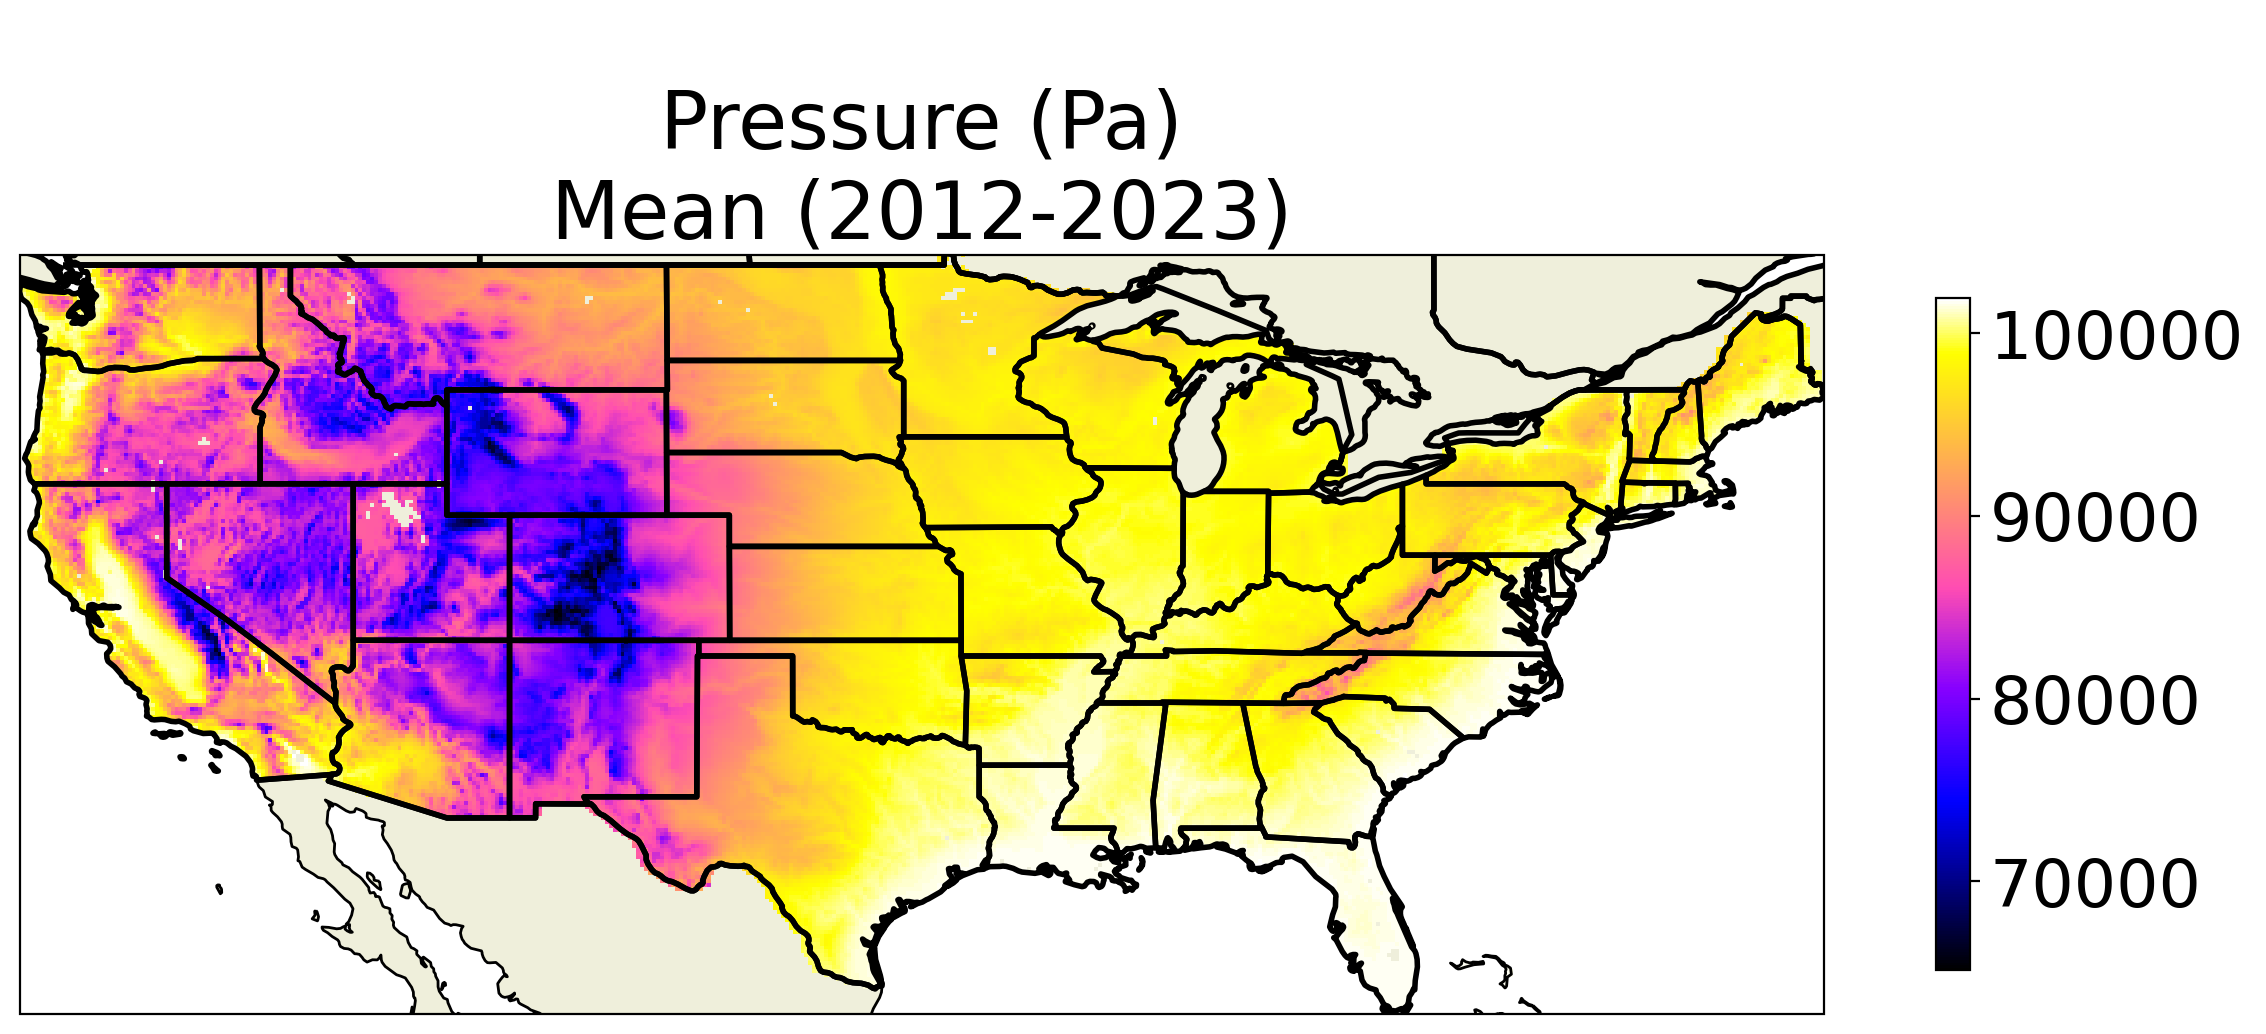
\includegraphics[width=.48\linewidth]{figures/thesis-gridstats/gridstat-bulk_pres_2012-1_2023-12_y000-195_x000-462_mean.png}
    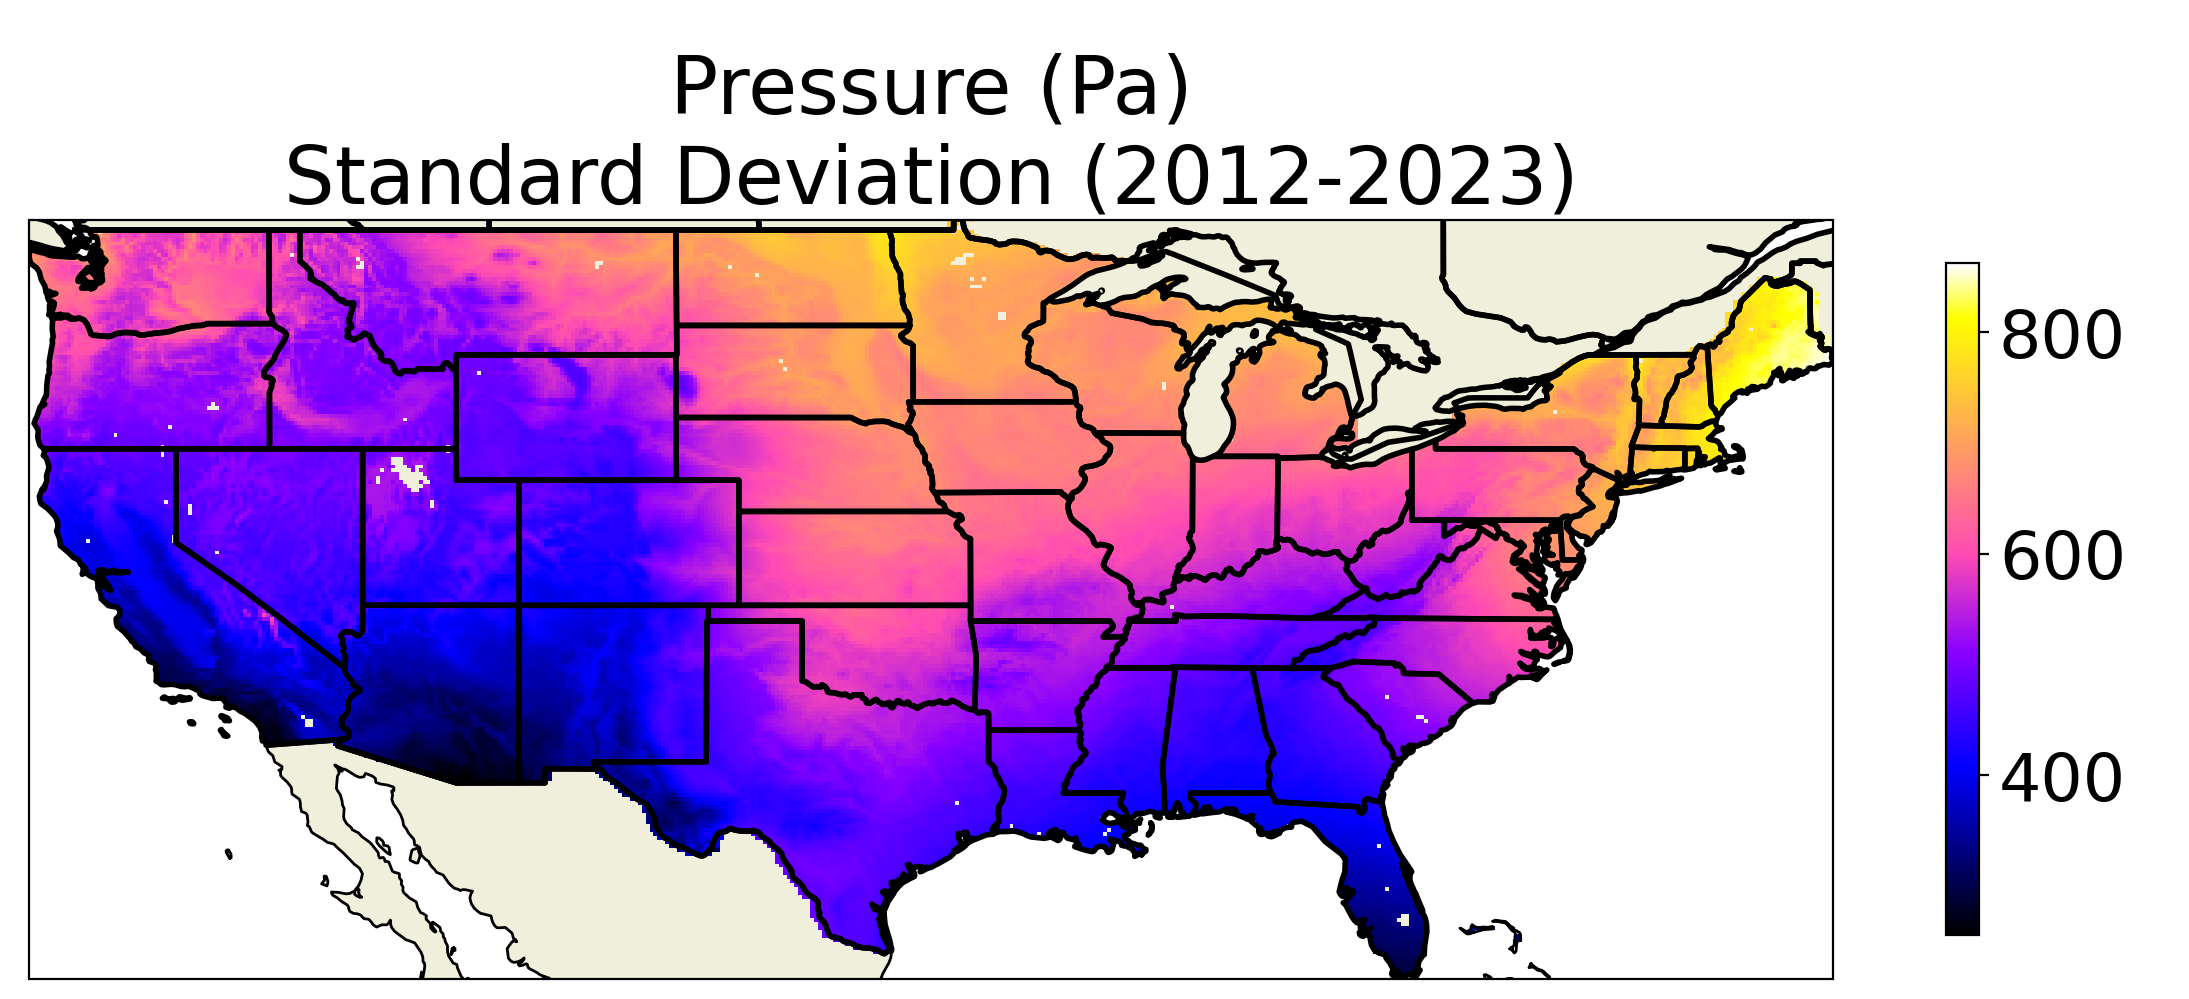
\includegraphics[width=.48\linewidth]{figures/thesis-gridstats/gridstat-bulk_pres_2012-1_2023-12_y000-195_x000-462_stdev.png}

    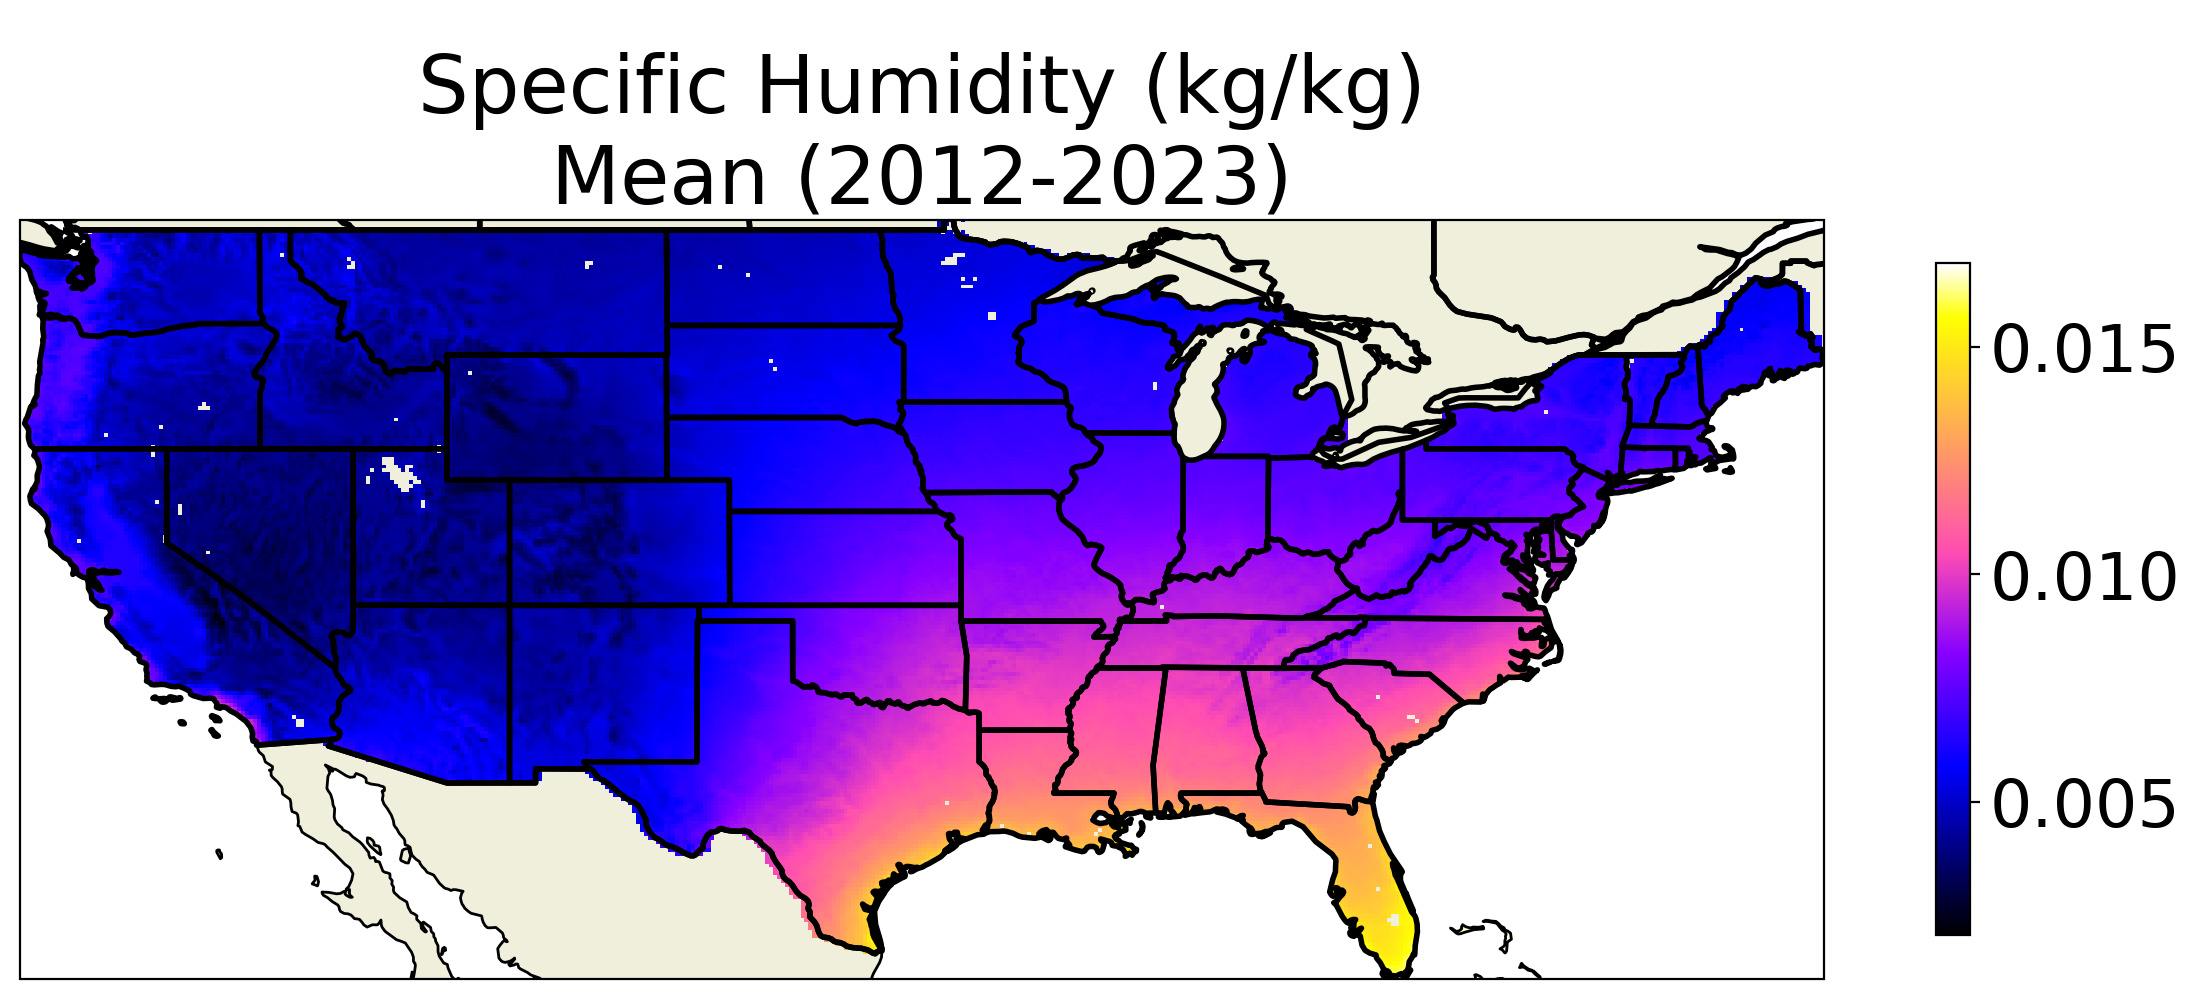
\includegraphics[width=.48\linewidth]{figures/thesis-gridstats/gridstat-bulk_spfh_2012-1_2023-12_y000-195_x000-462_mean.png}
    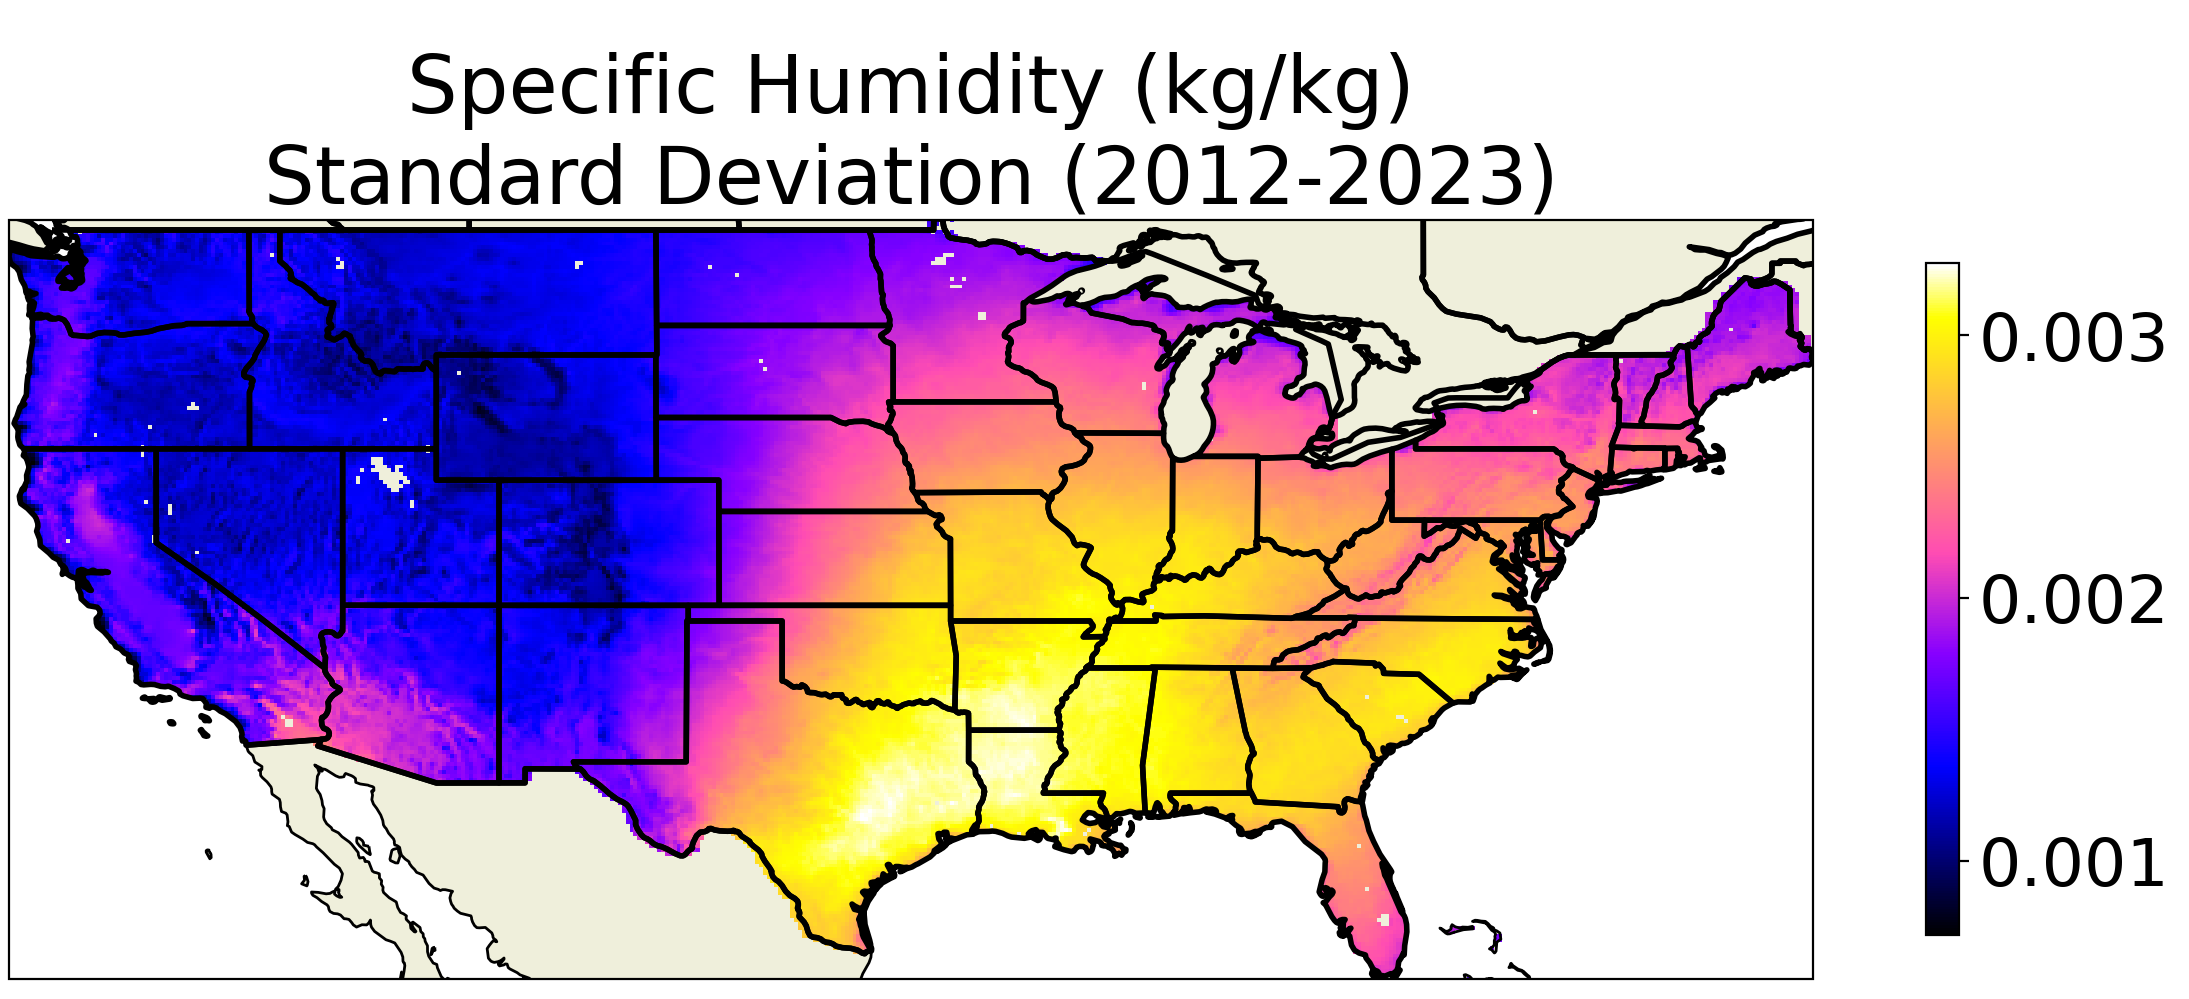
\includegraphics[width=.48\linewidth]{figures/thesis-gridstats/gridstat-bulk_spfh_2012-1_2023-12_y000-195_x000-462_stdev.png}

    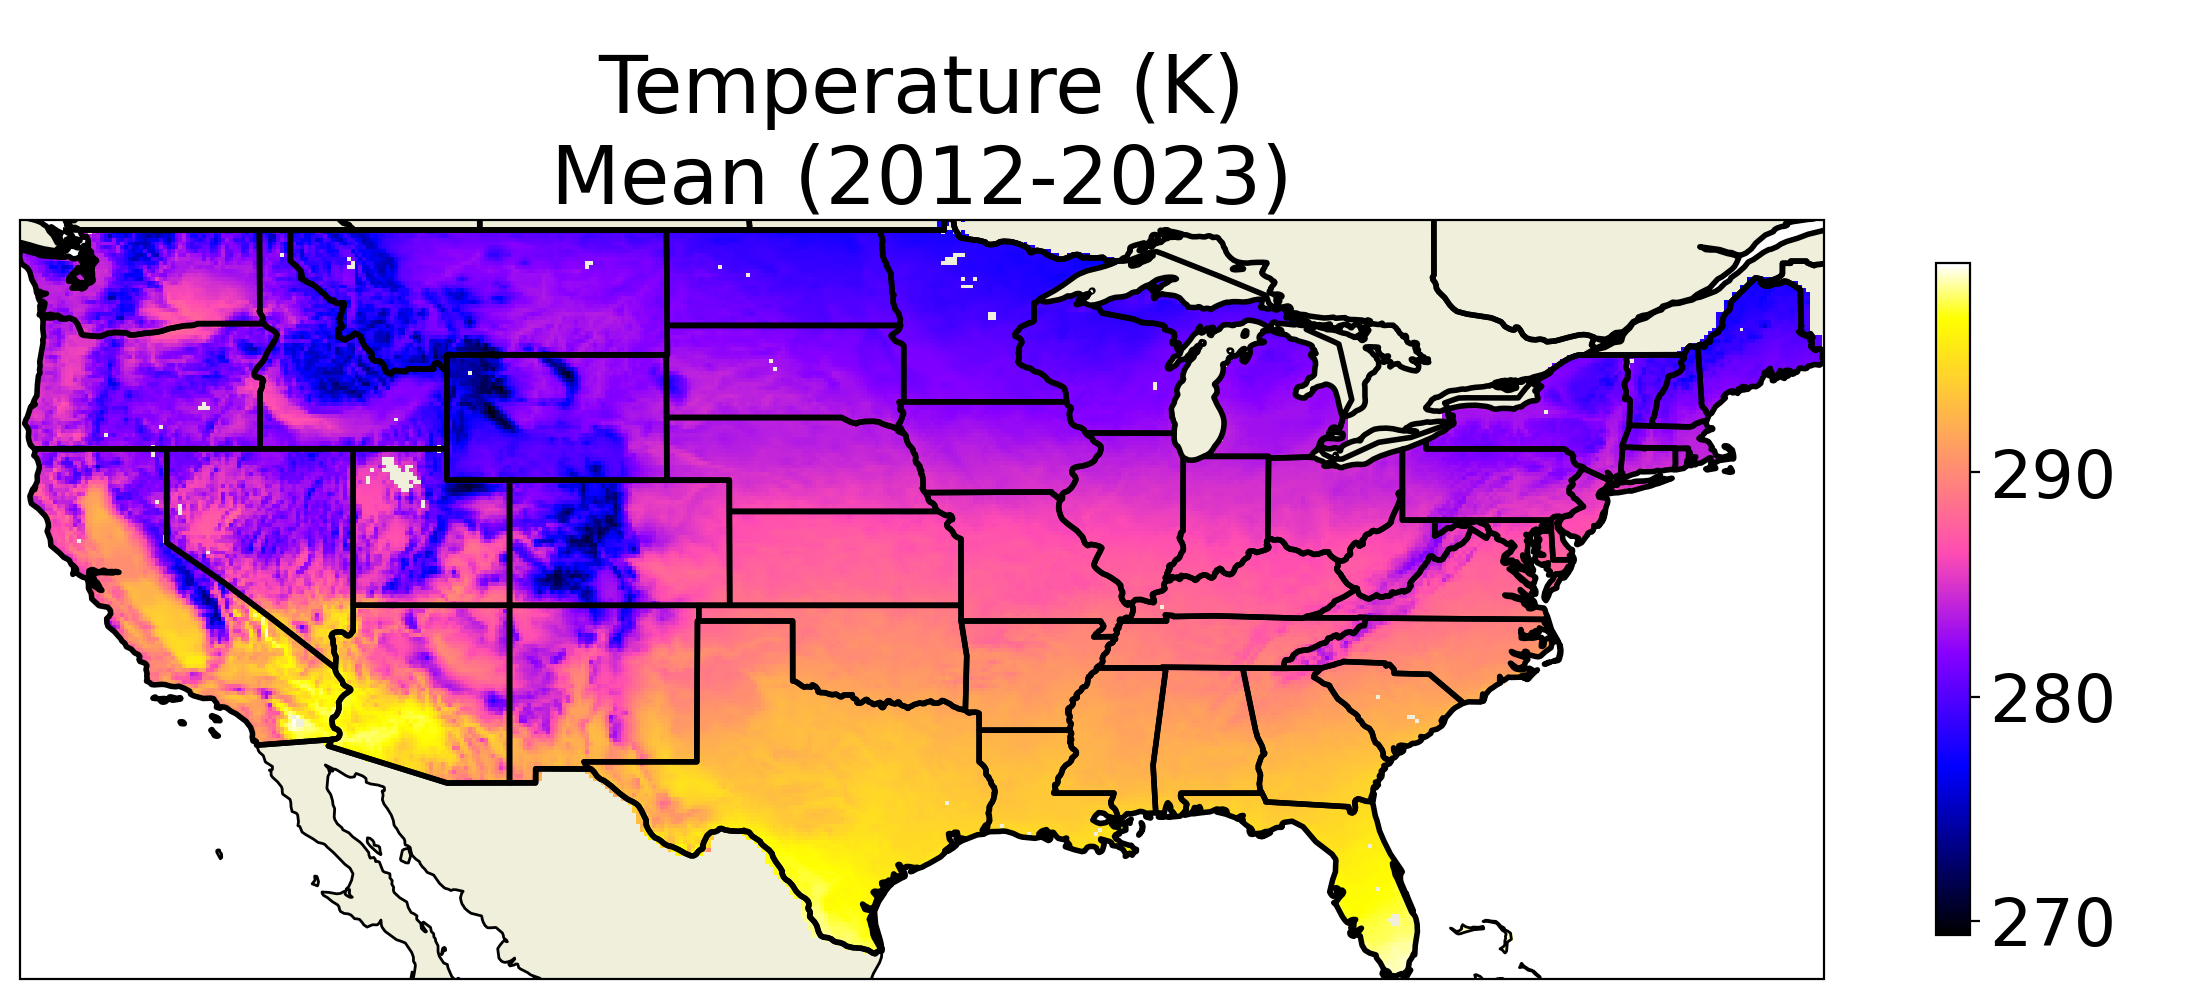
\includegraphics[width=.48\linewidth]{figures/thesis-gridstats/gridstat-bulk_tmp_2012-1_2023-12_y000-195_x000-462_mean.png}
    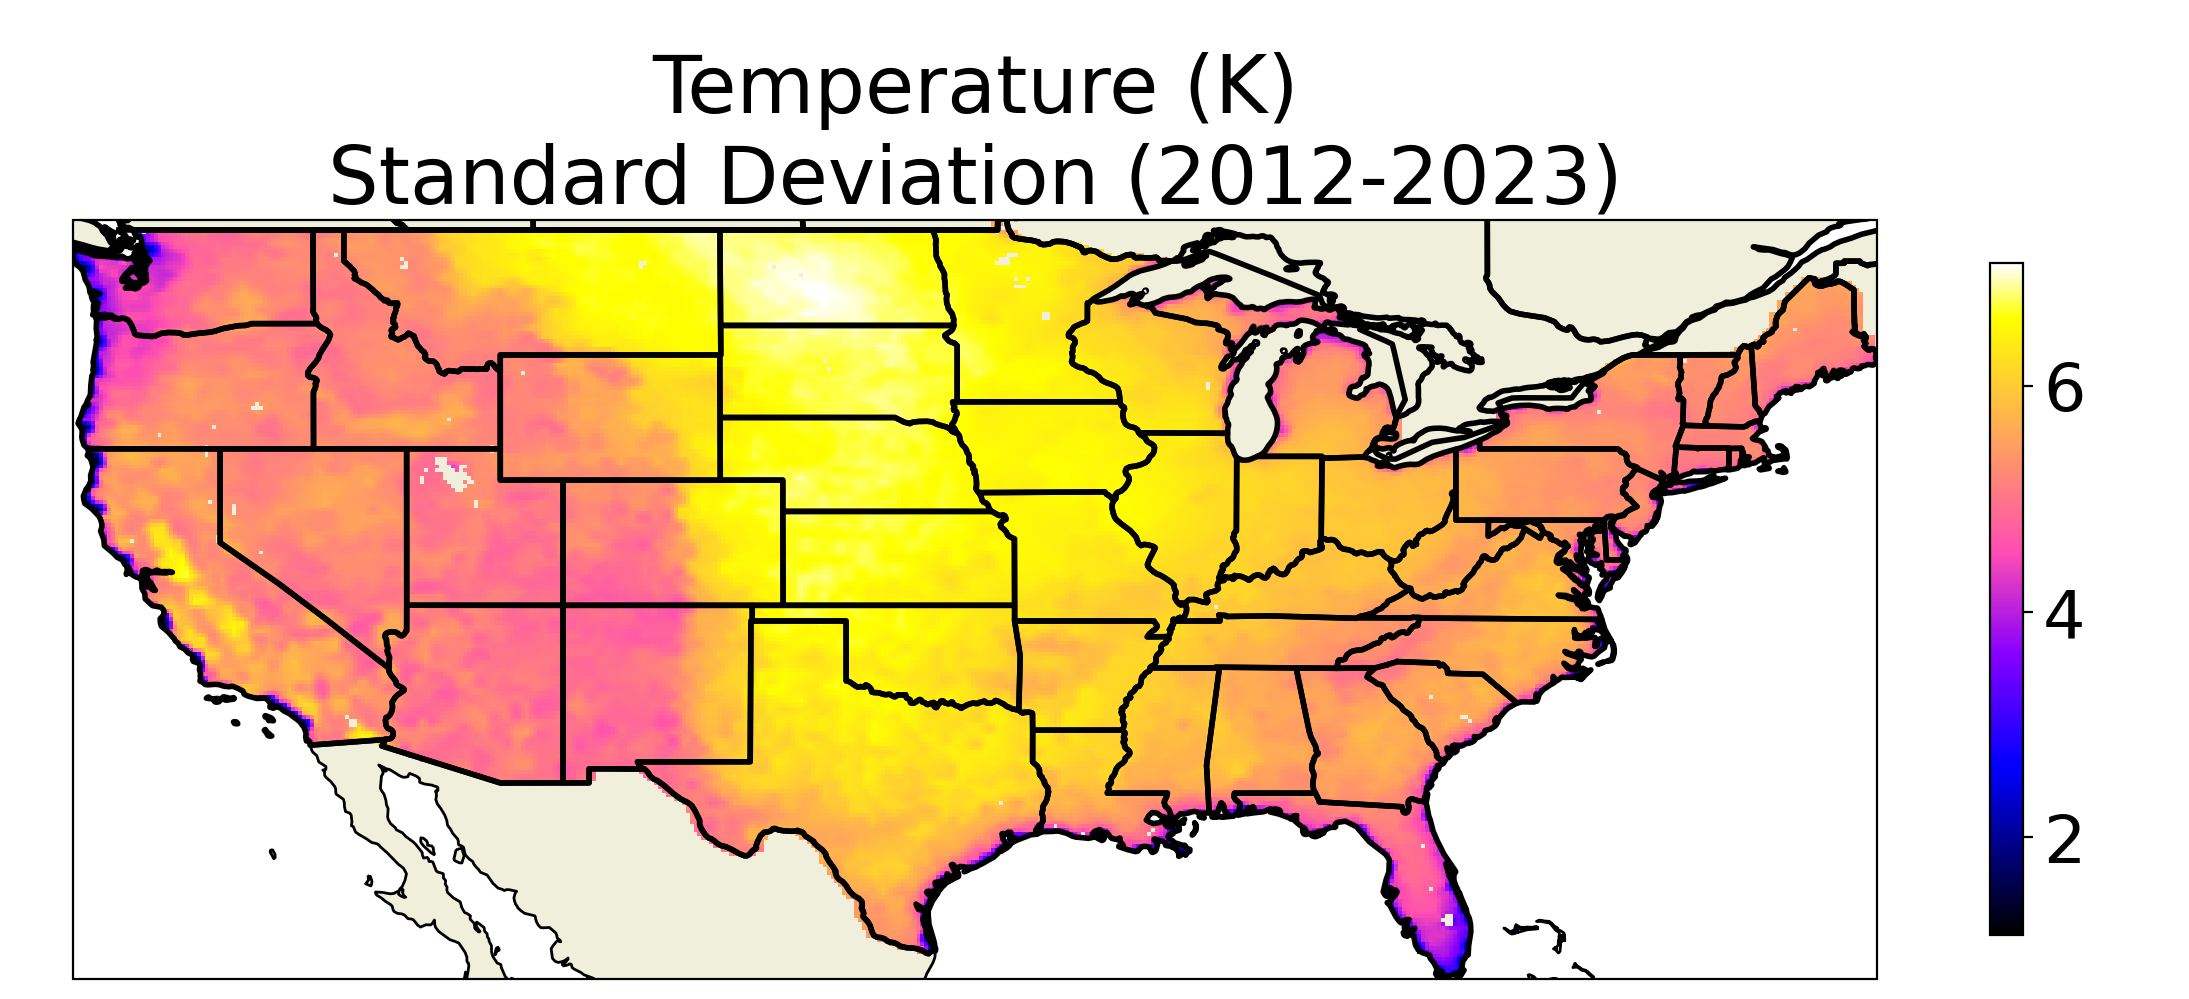
\includegraphics[width=.48\linewidth]{figures/thesis-gridstats/gridstat-bulk_tmp_2012-1_2023-12_y000-195_x000-462_stdev.png}

    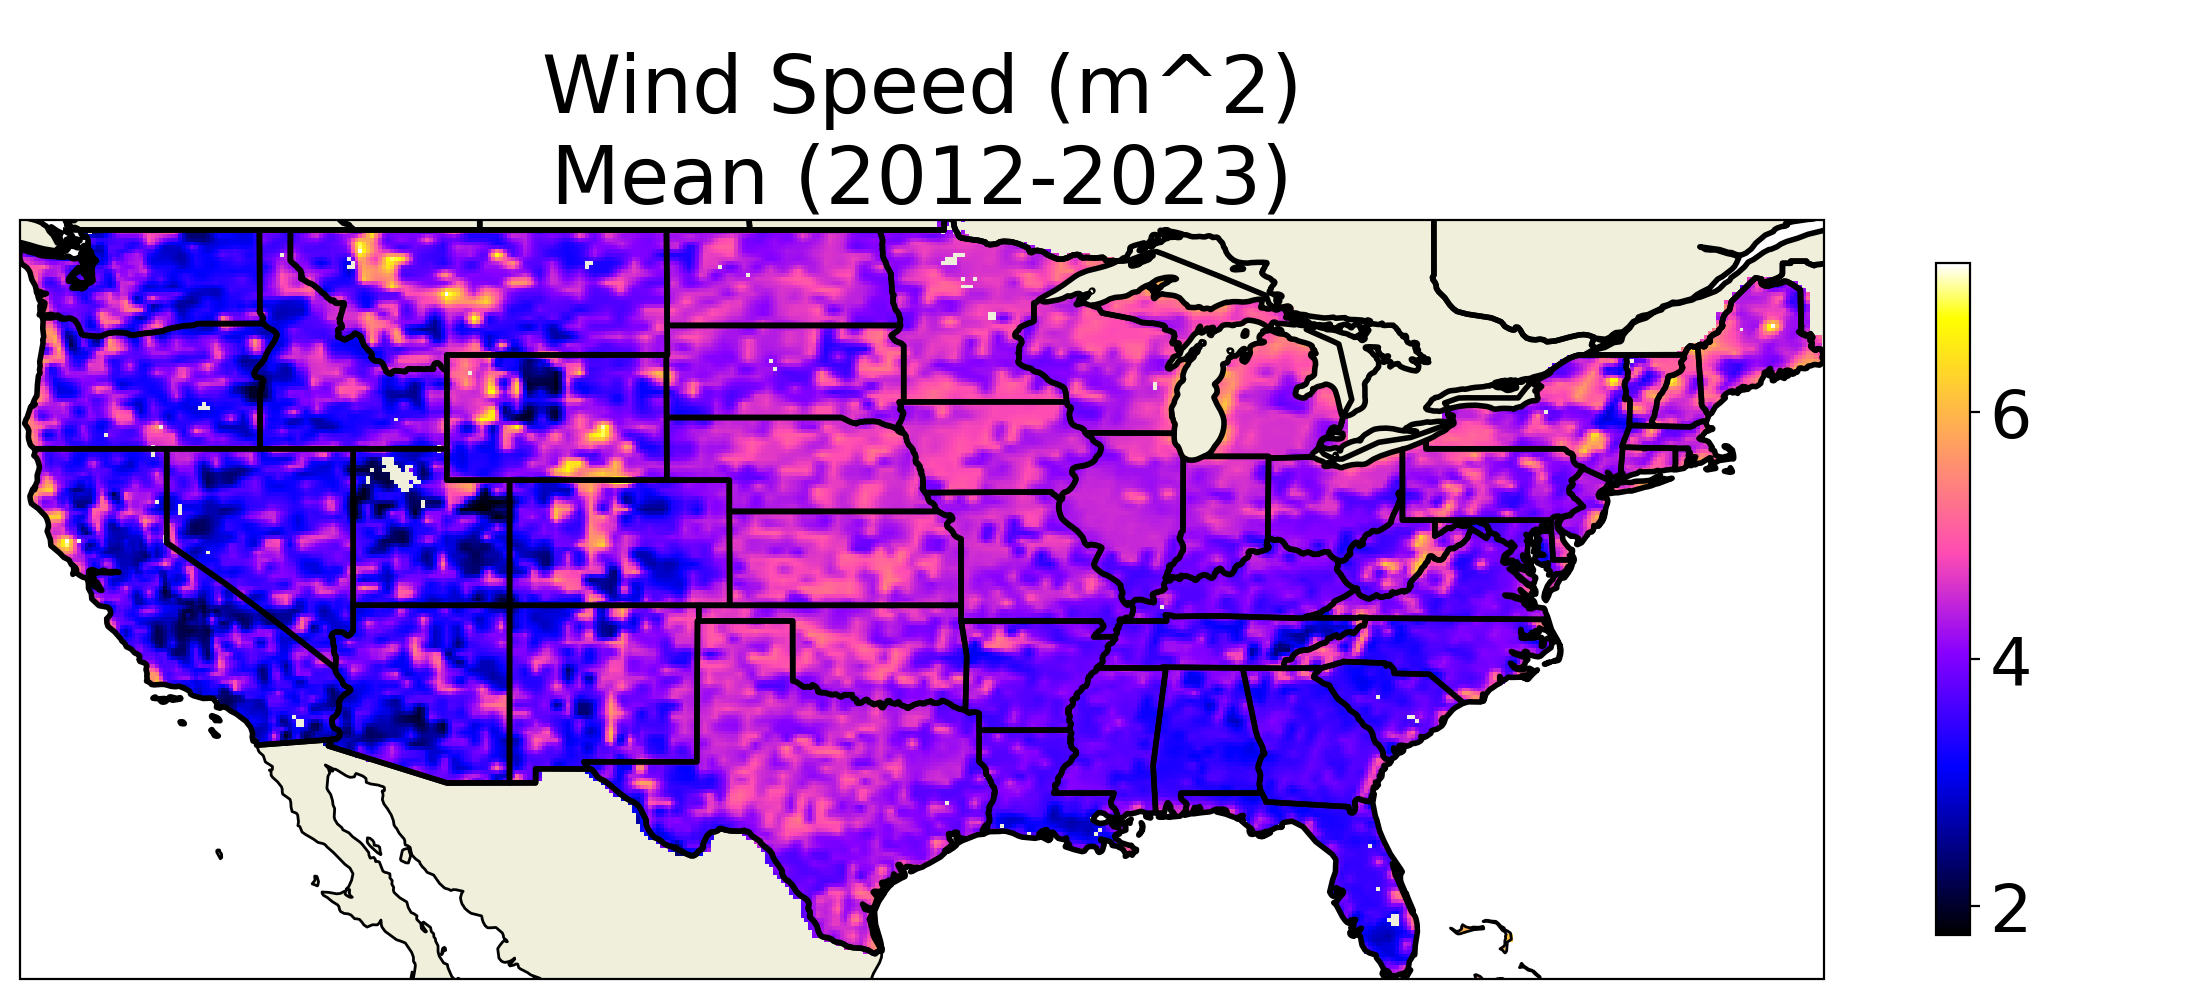
\includegraphics[width=.48\linewidth]{figures/thesis-gridstats/gridstat-bulk_windmag_2012-1_2023-12_y000-195_x000-462_mean.png}
    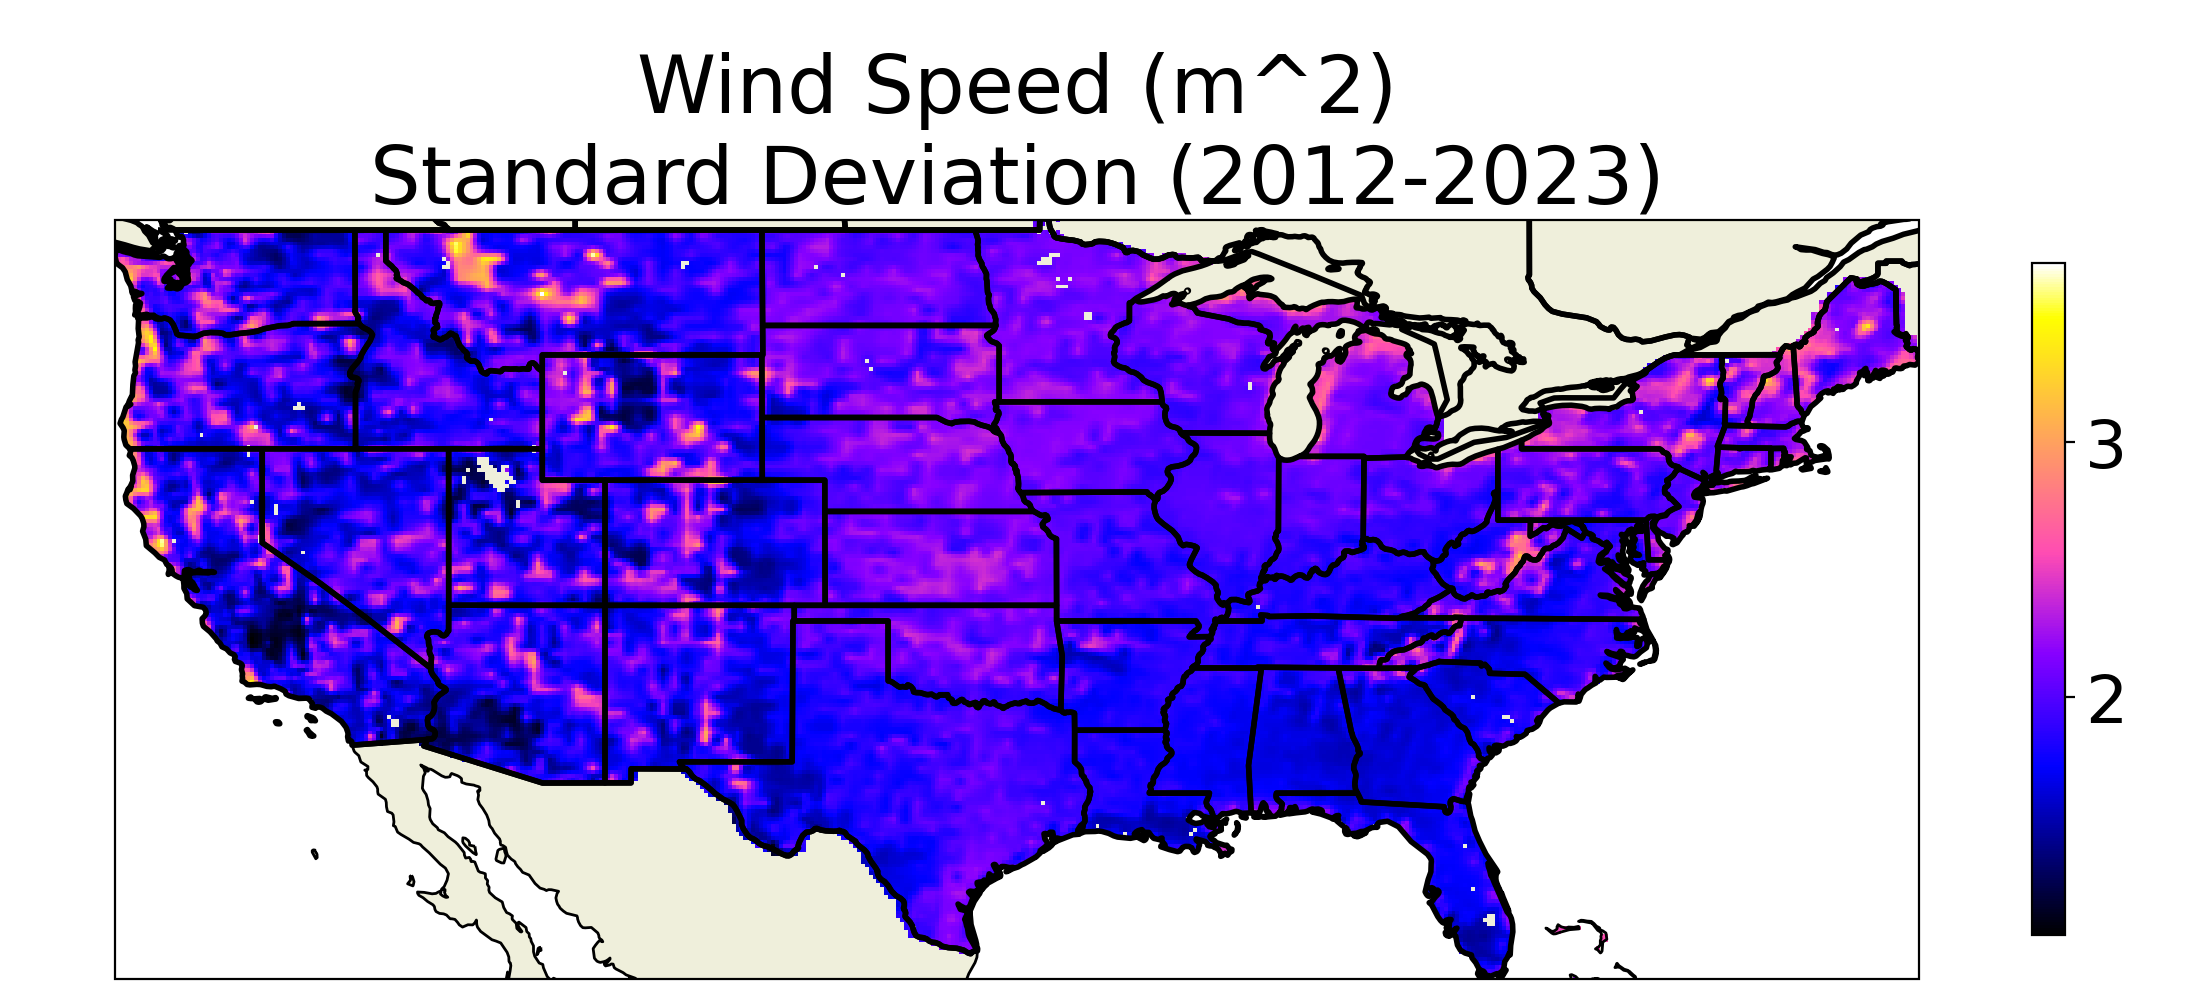
\includegraphics[width=.48\linewidth]{figures/thesis-gridstats/gridstat-bulk_windmag_2012-1_2023-12_y000-195_x000-462_stdev.png}
    \caption{Gridded mean and standard deviation of input forcings (2012-2023)}
    \label{gs-forcings}
\end{figure}

Figure \ref{gs-forcings} displays the same statistics for each of the other input forcings. The precipitation dataset includes liquid rain and snow, and reflects that the highest average values fell in the Pacific Coastal, Cascade, and Sierra Nevada, followed by more moderate values in the broad expanse of the Southeast, with the deep south of Louisiana and Mississippi seeing the strongest variability in precipitation throughout the year. Pressure mainly correlates with altitude, and higher latitudes tend to see the most variance, likely due to the prolonged influence of Rossby waves. Humidity and temperature also strongly correlate with temperature and proximity to the warm gulf, where the highest humidity variance is in the southern states thanks to seasonal intrusions of warm, moist air. The highest temperature variance is found in the high plains where there are considerable intrusions of arctic air in the winter, and solar heating combined with warm air advection from the terrain-driven low level jet in the summer. The wind is locally strongest where there is channeling from mountain slopes, with a broad region of relatively high wind speeds in the plains due to the open terrain.

\subsection{Handling Snow}

\begin{figure}[hb!]
    \centering
    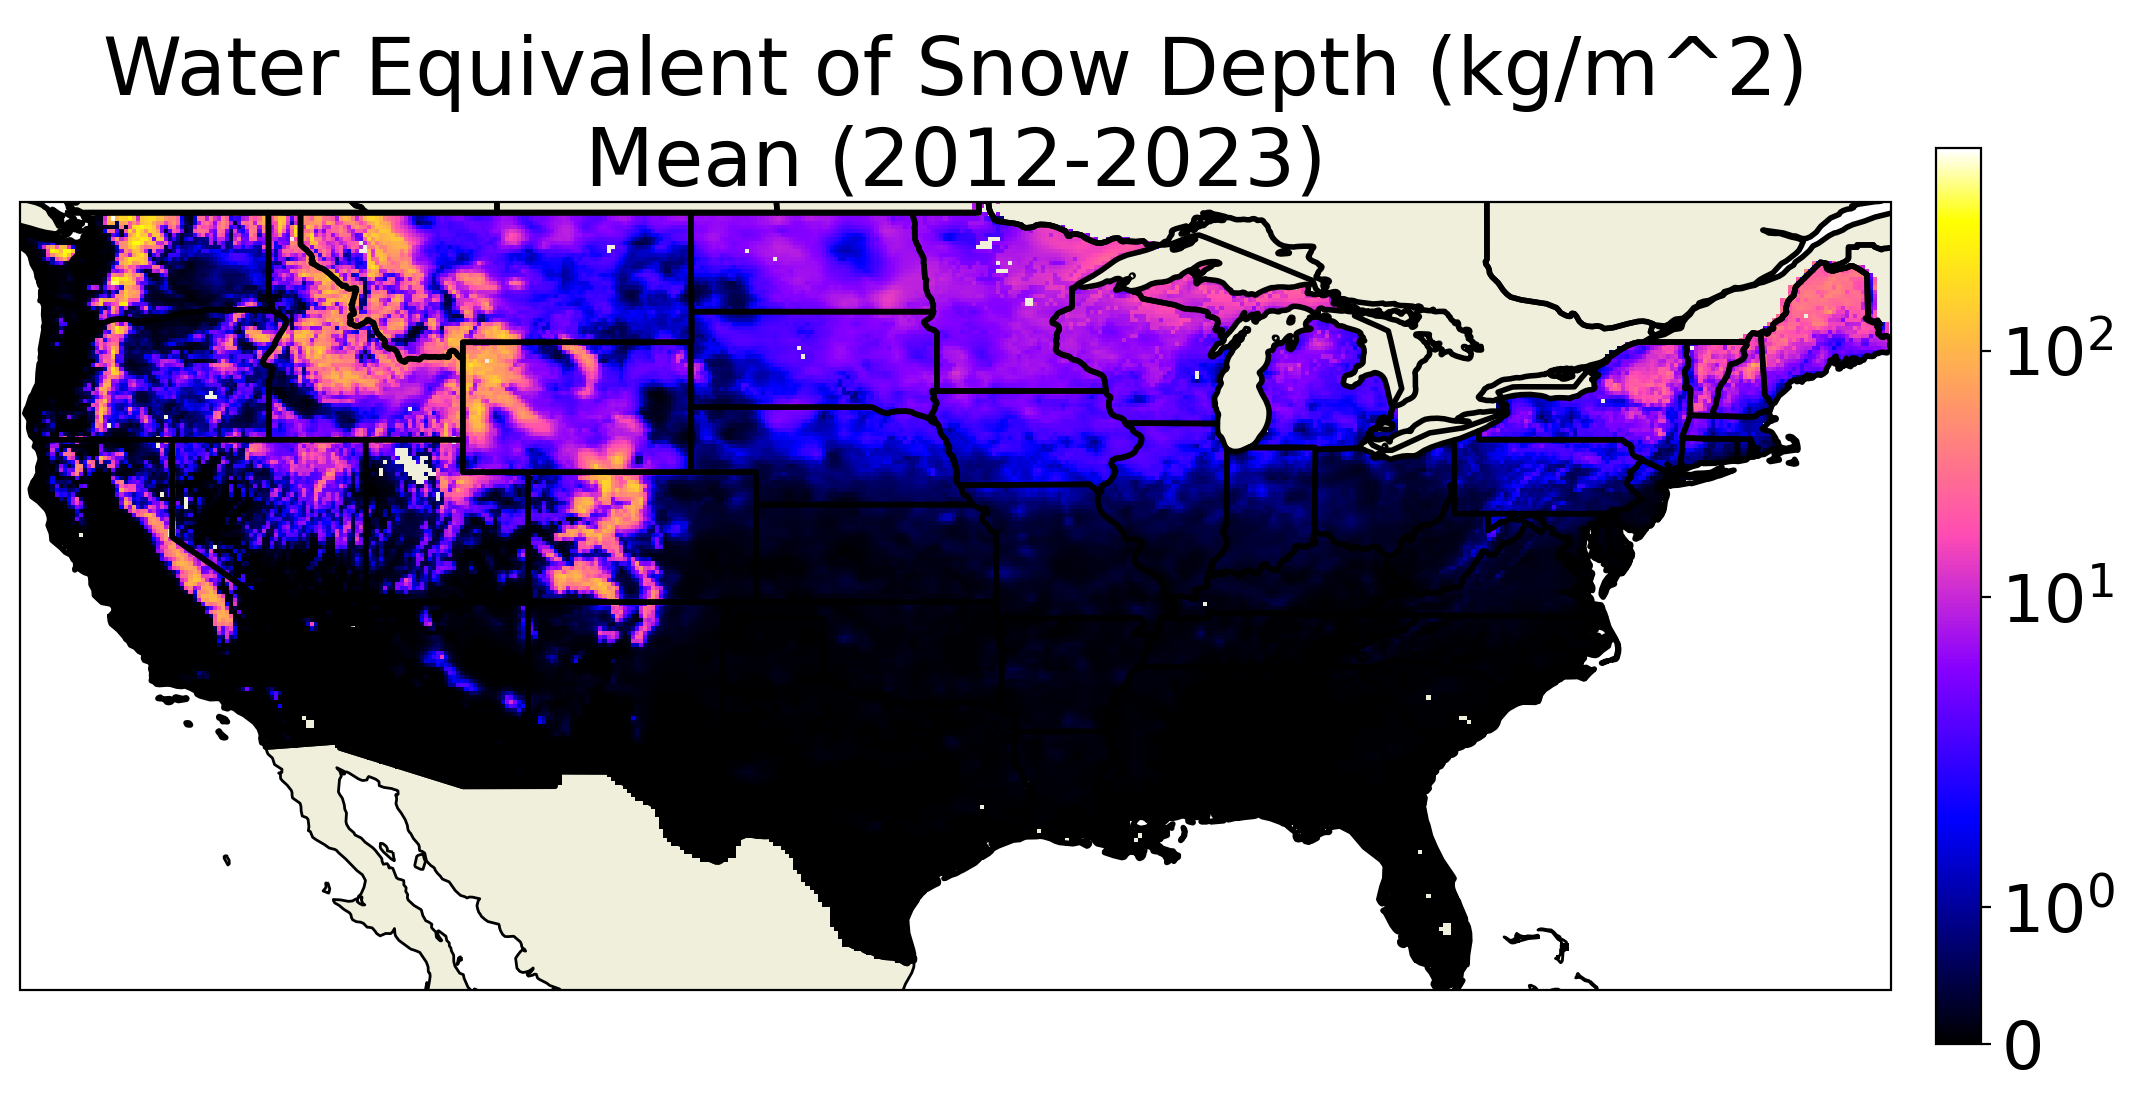
\includegraphics[width=.48\linewidth]{figures/thesis-gridstats/gridstat-bulk_weasd-log_2012-1_2023-12_y000-195_x000-462_mean.png}
    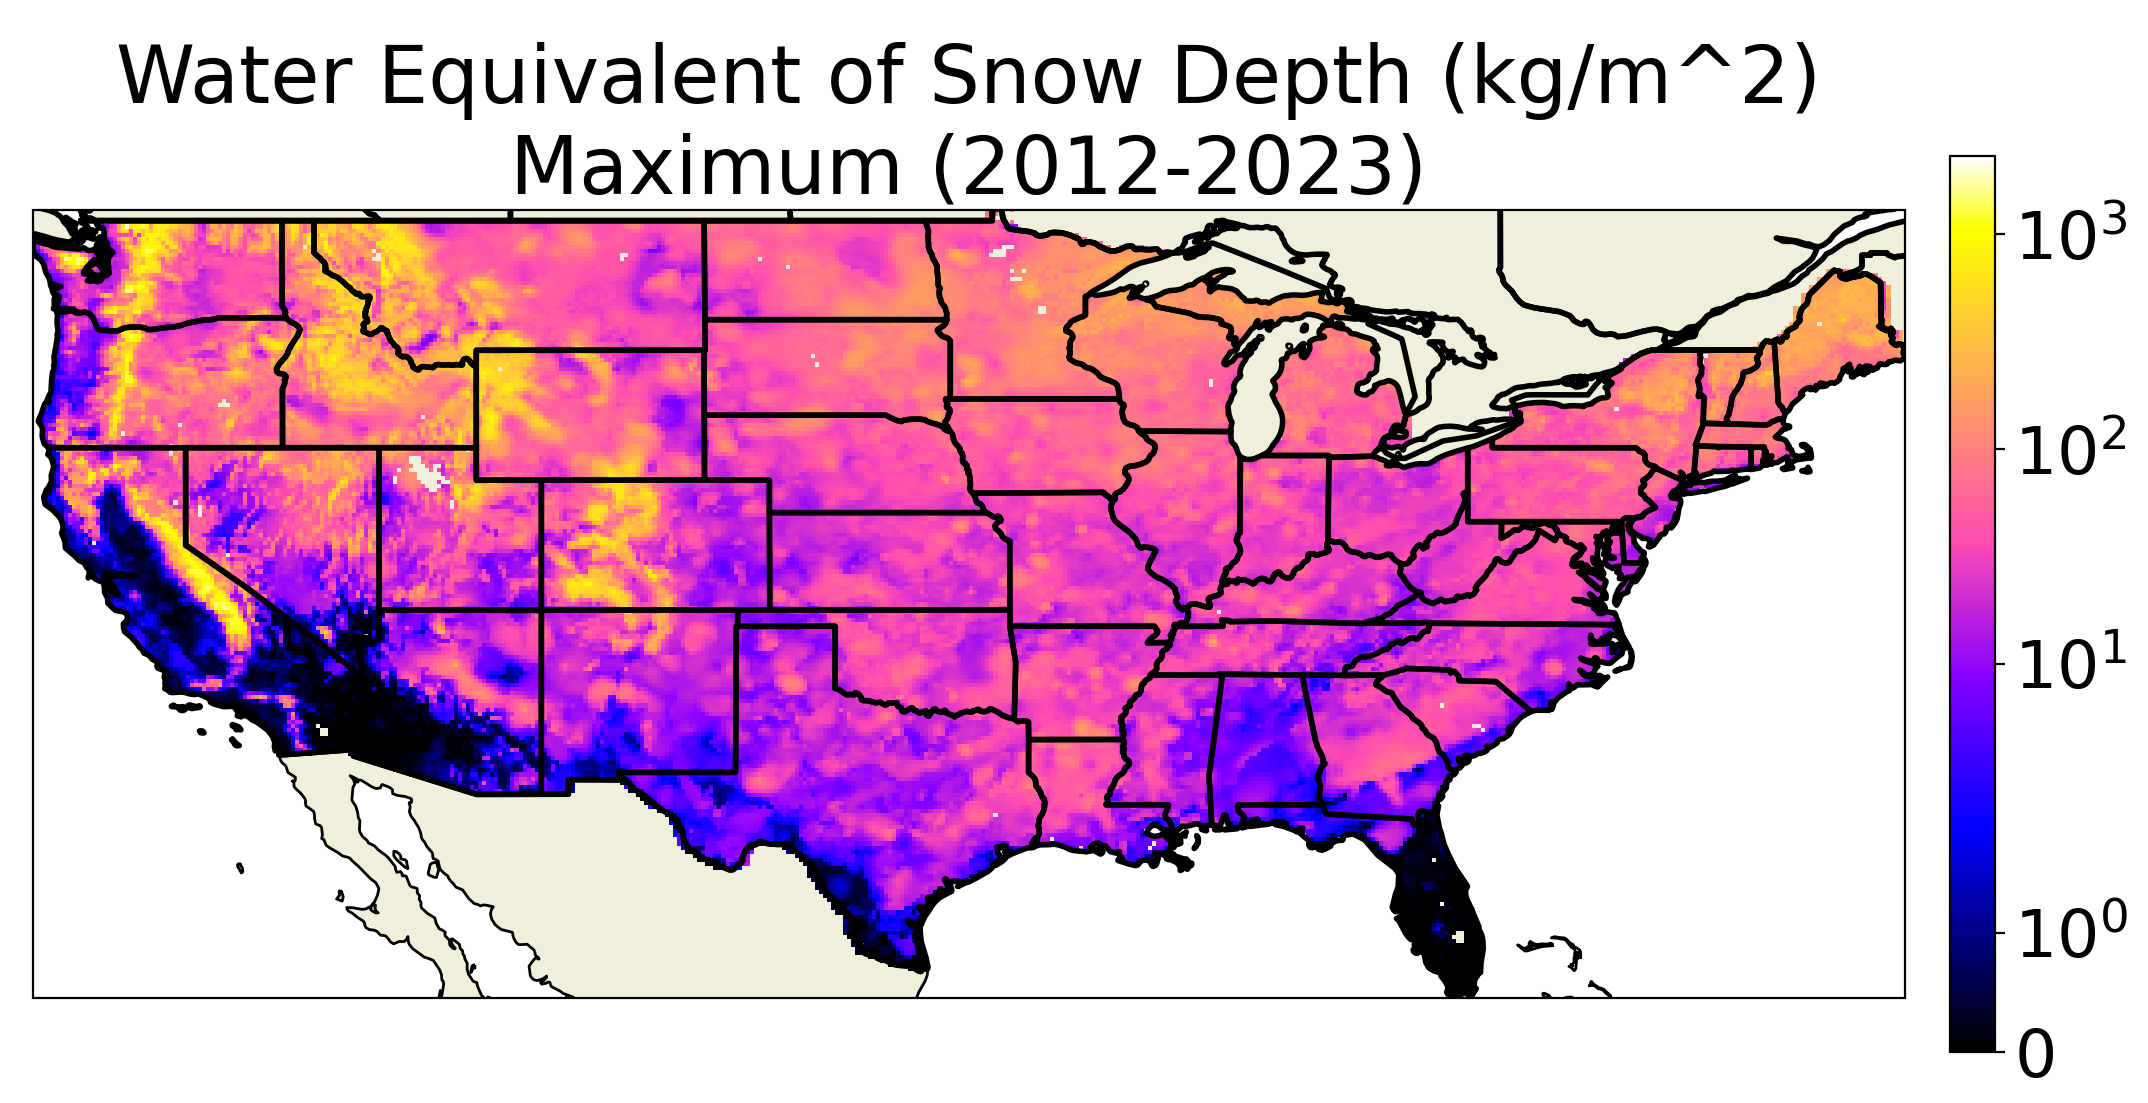
\includegraphics[width=.48\linewidth]{figures/thesis-gridstats/gridstat-bulk_weasd-log_2012-1_2023-12_y000-195_x000-462_max.png}
    \caption{Mean and maximum accumulated snow amounts on a log scale (2012-2023)}
    \label{gs-snow}
\end{figure}

Figure \ref{gs-snow} shows the mean and maximum snow accumulation throughout the dataset. Snow is particularly difficult to account for in the ANNs because it is relatively rare and highly regional, but has a profound influence on the soil dynamics. The presence of snow significantly modifies the surface albedo and roughness length, captures and stores precipitation as an additional state variable, and represents a new source of water for the soil column as it melts \citep{koren_parameterization_1999}. The first exploratory models we trained treated snow as essentially an additional soil layer, and predicted the increment change in its value alongside the other soil states. Since snow is such a transient phenonmenon within the training dataset the ANNs would consistently predict close to zero change, even in snowy conditions, since doing so results in the lowest loss in most cases.

\begin{figure}[hb!]
    \centering
    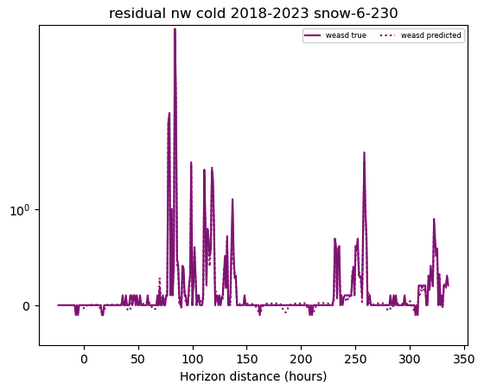
\includegraphics[width=.32\linewidth]{figures/snow-sample_res.png}
    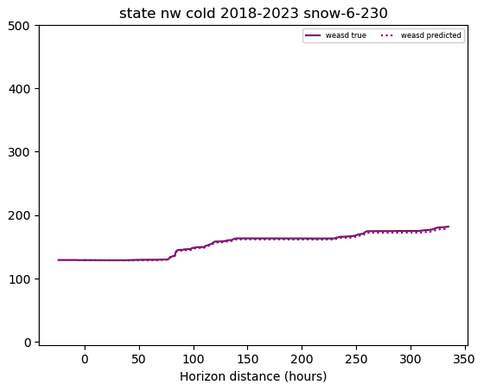
\includegraphics[width=.32\linewidth]{figures/snow-sample_state.png}
    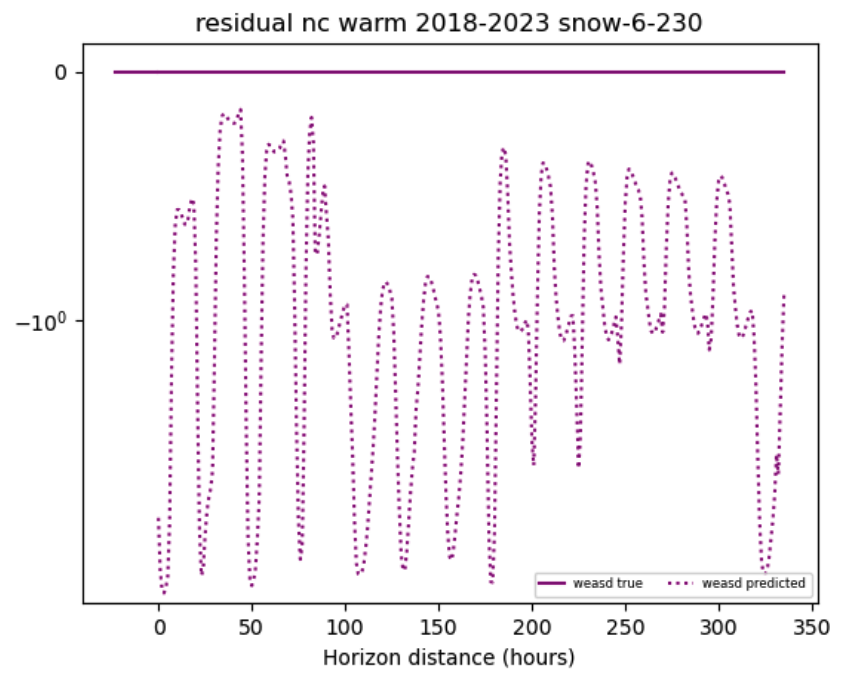
\includegraphics[width=.32\linewidth]{figures/snow-sample_warm.png}
    \caption{Samples of snow-only model predictions vs true values after loss function manipulation, including the increment change for a significant snowfall event (left), the accumulated state for the same sample (center), and an example of the increment outputs of a different warm-season sample (right).}
    \label{snow-models}
\end{figure}

Subsequent models trained to exclusively target the increment change in snow water equivalent showed the same hesitancy to make non-zero predictions. In order to loosen the requirement that these models must always output zero change when there is no snow present, we modified the loss function used to train the snow-only models such that predicting negative increment change values when there is no snow present will not be penalized. When combined with a post-processing step that truncates negative accumulated snow amounts at zero, this strategy focuses the gradient descent process exclusively on samples where the snow pack is relevant.

Figure \ref{snow-models} displays a sample from one of these loss-modified snow models, which captures the subtleties of extreme snow events, and maintains negative increment predictions when there is no snow present or accumulating. Curiously, the negative predictions of the model during the warm-season sample cycle on a diurnal basis, and may represent a hypothetical snow melt rate, which is an emergent property since the loss function wasn't applied in such scenarios. In any case, although these are encouraging preliminary results, further refinement of this strategy is out of the scope of this project. We will use the true snow amount as an input to the soil moisture ANNs presented here in order to prevent compounding error, and take the apparent validity of this approach as an indication that separate ANNs designed specifically for snow water equivalent estimation may be used to initialize soil moisture emulators in the future.

\subsection{Input Data Value Distributions}

\begin{figure}[hb!]
    \centering
    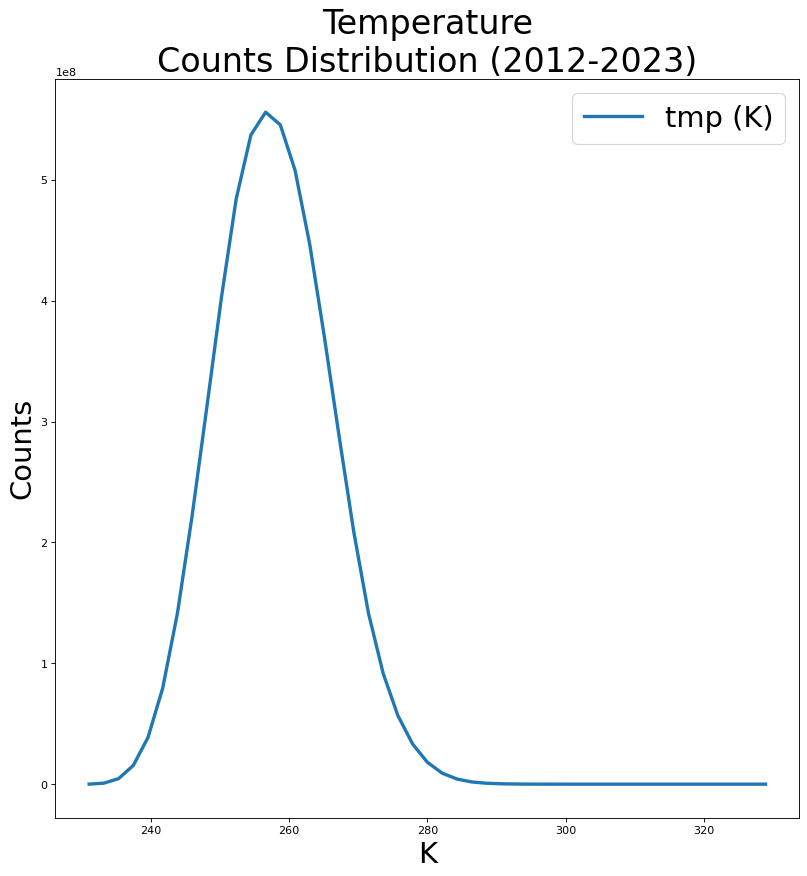
\includegraphics[width=.24\linewidth]{figures/thesis-gridstats/gridstat-hist_tmp_2012-1_2023-12_y000-195_x000-462.png}
    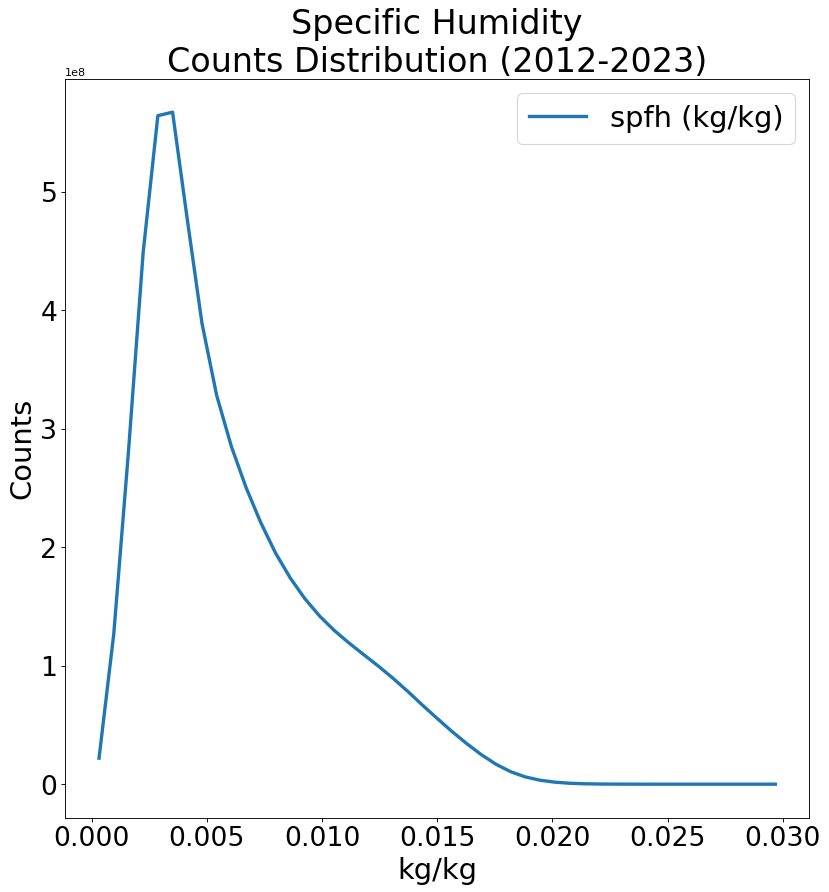
\includegraphics[width=.24\linewidth]{figures/thesis-gridstats/gridstat-hist_spfh_2012-1_2023-12_y000-195_x000-462.png}
    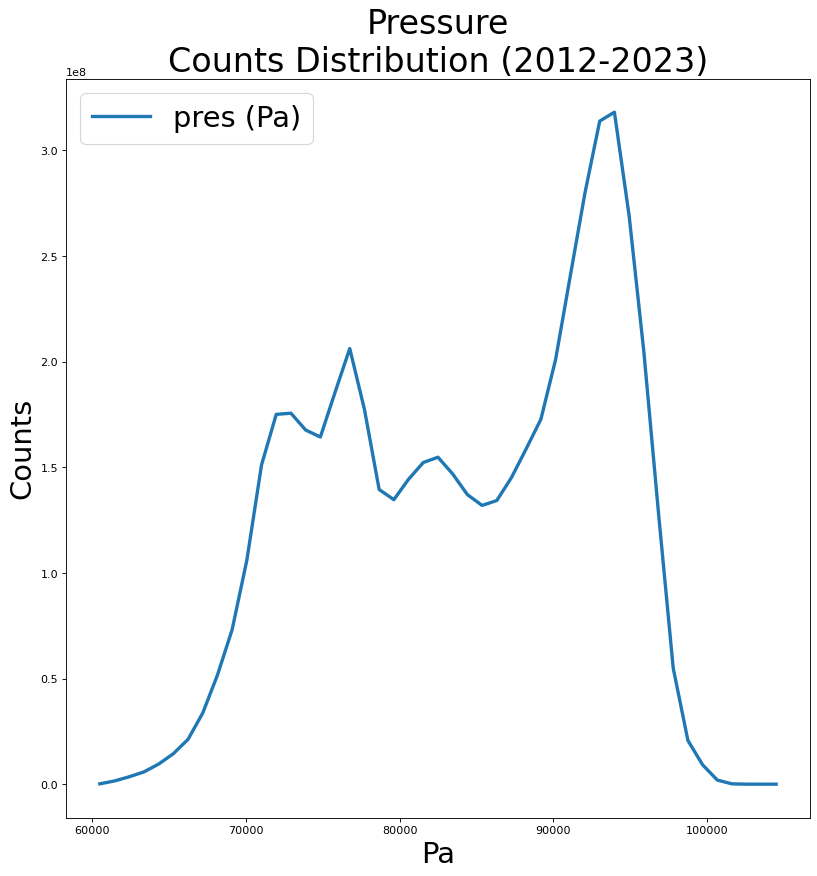
\includegraphics[width=.24\linewidth]{figures/thesis-gridstats/gridstat-hist_pres_2012-1_2023-12_y000-195_x000-462.png}
    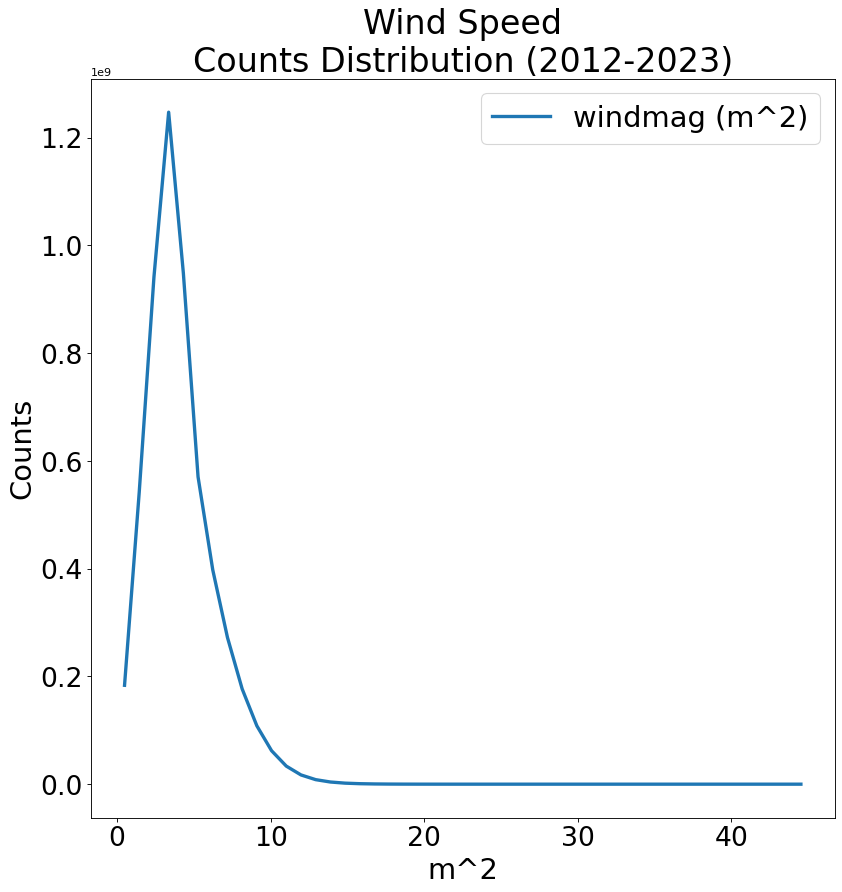
\includegraphics[width=.24\linewidth]{figures/thesis-gridstats/gridstat-hist_windmag_2012-1_2023-12_y000-195_x000-462.png}

    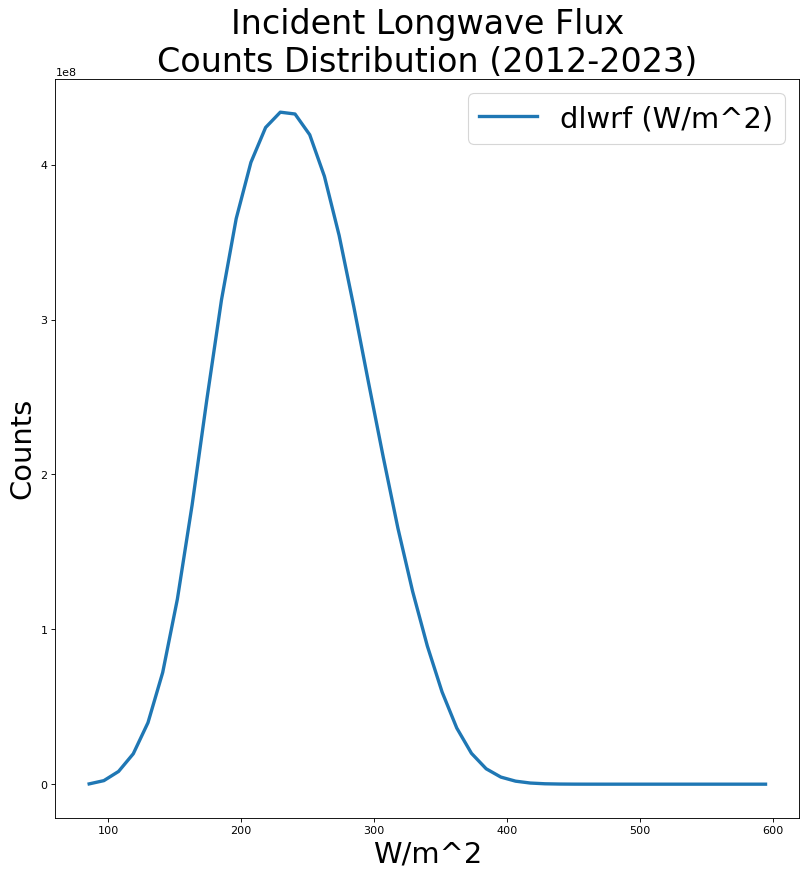
\includegraphics[width=.24\linewidth]{figures/thesis-gridstats/gridstat-hist_dlwrf_2012-1_2023-12_y000-195_x000-462.png}
    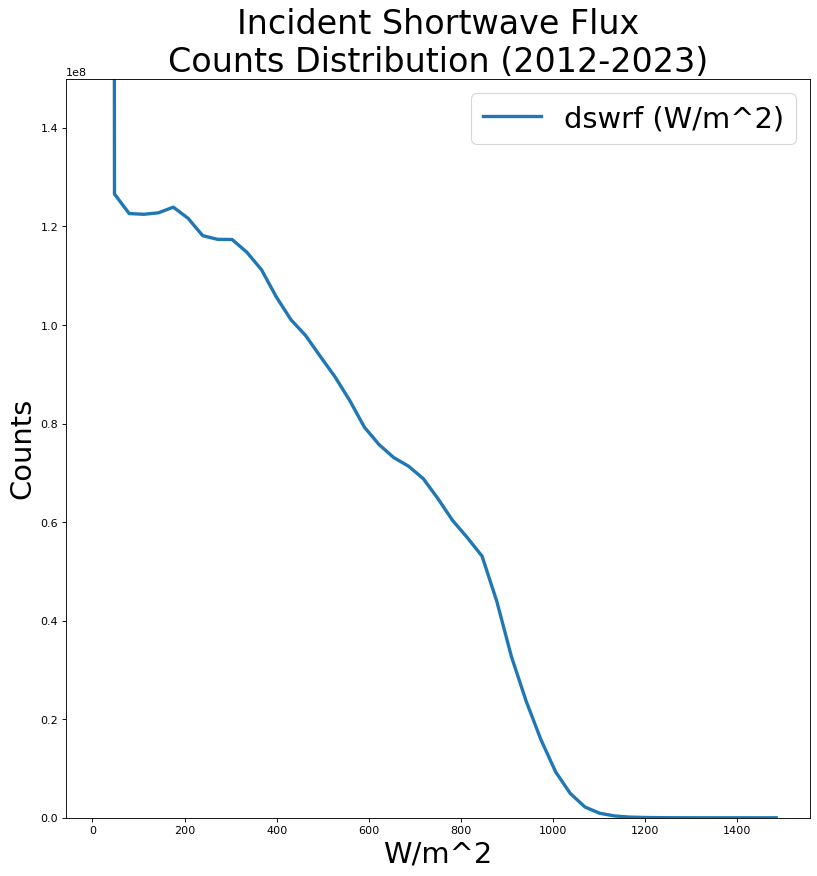
\includegraphics[width=.24\linewidth]{figures/thesis-gridstats/gridstat-hist_dswrf_2012-1_2023-12_y000-195_x000-462.png}
    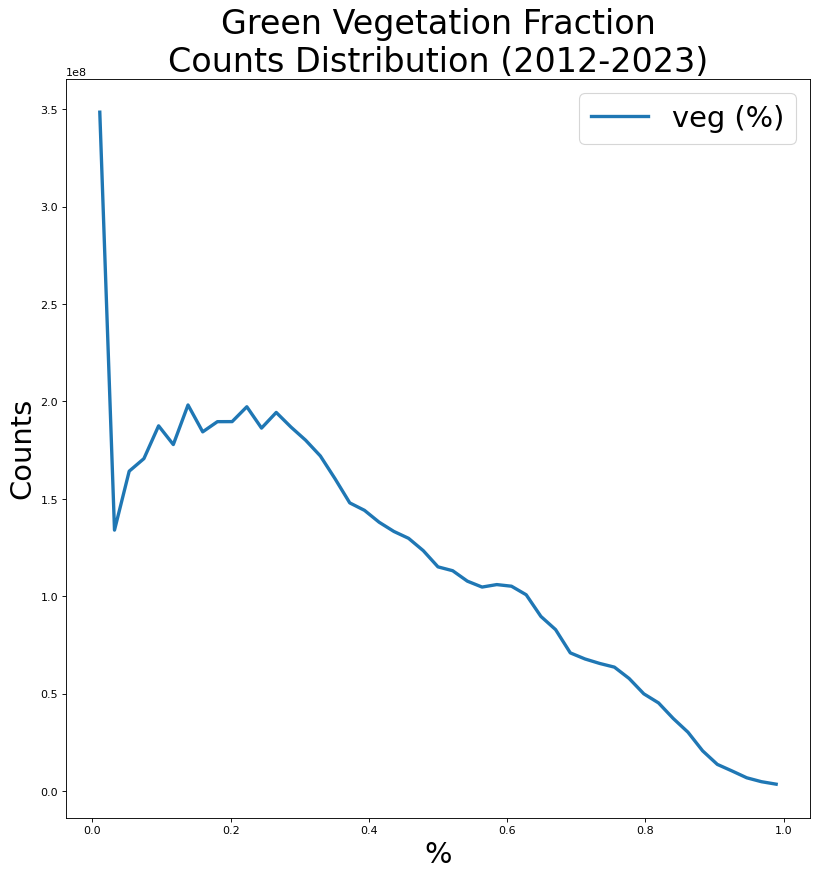
\includegraphics[width=.24\linewidth]{figures/thesis-gridstats/gridstat-hist_veg_2012-1_2023-12_y000-195_x000-462.png}
    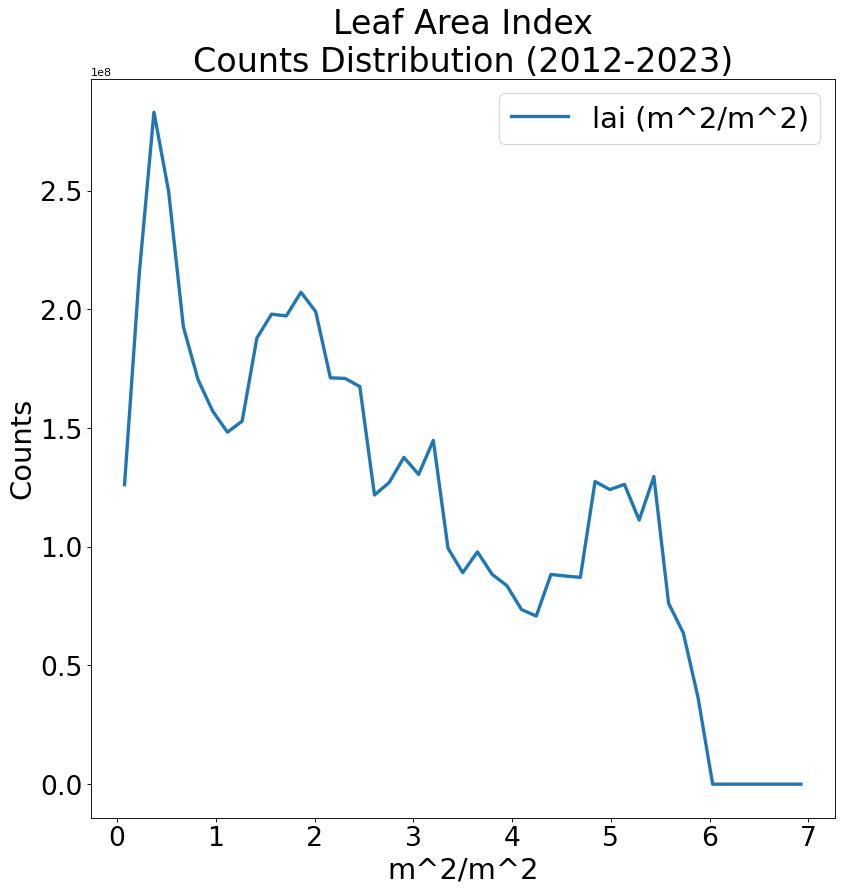
\includegraphics[width=.24\linewidth]{figures/thesis-gridstats/gridstat-hist_lai_2012-1_2023-12_y000-195_x000-462.png}

    \caption{Overall distributions of dynamic model inputs (2012-2023)}
    \label{dist-forcings}
\end{figure}

The count distributions of dynamic inputs with the exception of precipitation are displayed by Figure \ref{dist-forcings}. Of these only temperature and incident longwave flux follow generally gaussian distributions. Specific humidity is strongly skewed toward zero since its upper bound is limited by temperature. Pressure has a global peak just below sea level pressure, with relative maxima associated with the mountainous terrain of Appalachia and the West. Windspeed has a strong peak around 5 $m s^{-1}$, with a long tail of outliers. Shortwave flux is not entirely smooth, which is likely due in part to enhanced cloud cover from orographic effects, judging by the spatial distribution in Figure \ref{gs-radiative}. The vegetation parameters are also strongly non-gaussian owing to their regional and seasonal heterogeneity, and the discrete differences in vegetation categories.


\begin{figure}[h!]
    \centering
    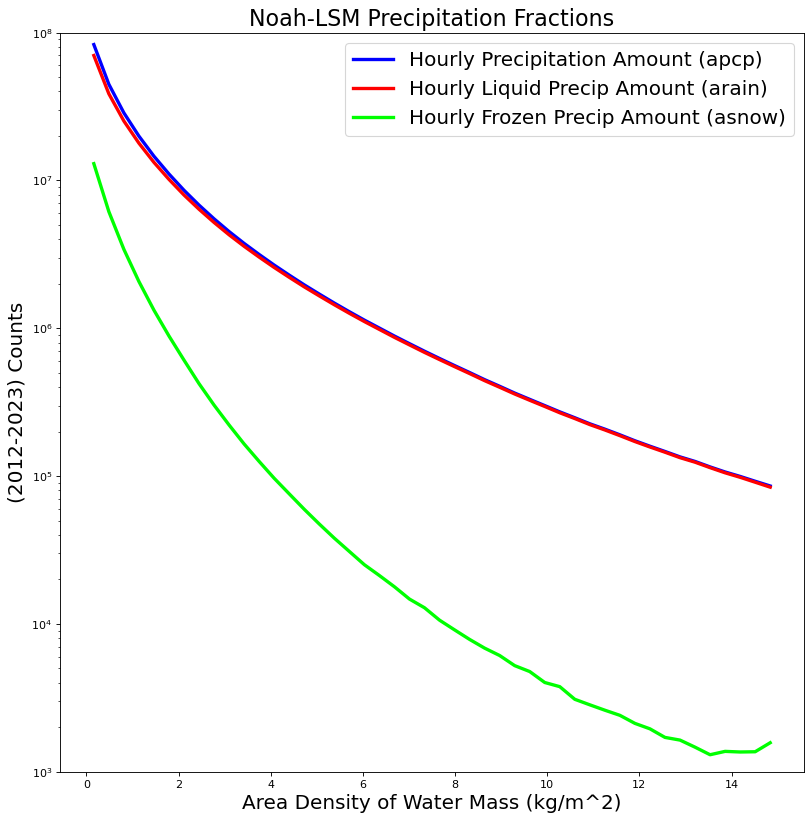
\includegraphics[width=.48\linewidth]{figures/thesis-gridstats/gridstat-hist_groupings_preciptype.png}
    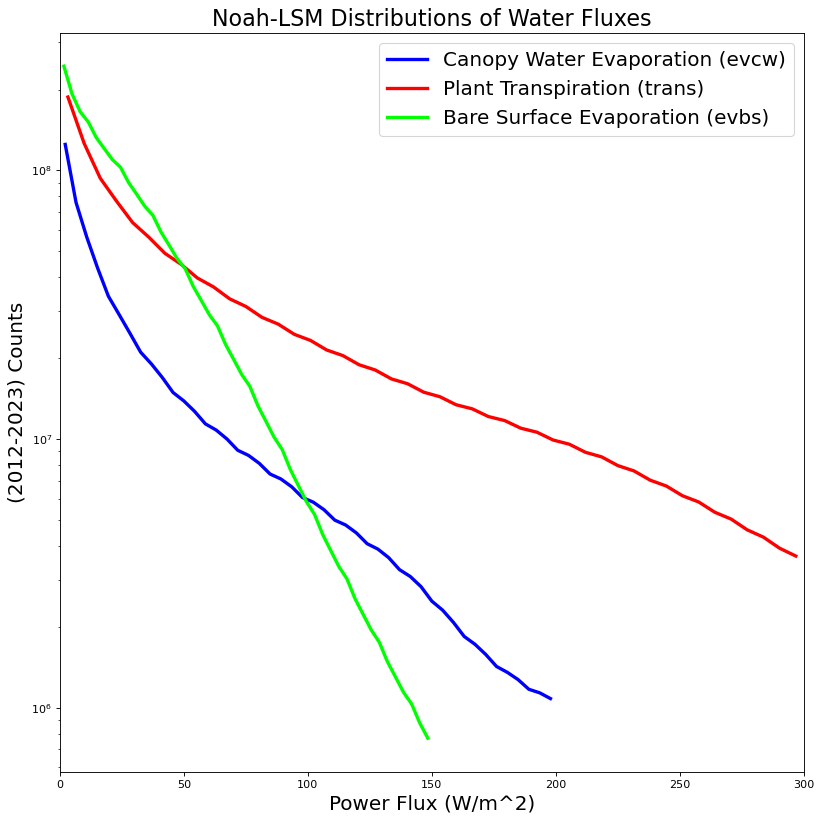
\includegraphics[width=.48\linewidth]{figures/thesis-gridstats/gridstat-hist_groupings_powerflux.png}
    \caption{Overall distributions of precipitation types (left) and fluxes removing water from the surface system (right), both on a logarithmic axis (2012-2023).}
    \label{dist-waterflux}
\end{figure}

Figure \ref{dist-waterflux} compares the distributions of precipitation types, and those of the fluxes that remove water from the system. Liquid precipitation represents the vast majority of the total hourly precipitation amount, especially for strong precipitation events. Plant transpiration is the dominant sink for soil moisture content, with bare surface evaporation mainly limited to lower rates. Evaporation from the plant canopy can also be relevant in mitigating the amount of water that percolated downward into the soil column after rain events. Each of the distributions extend further with higher-value outliers, however these were truncated during the statistic collection process in order to emphasize the shape of the more common lower-end values. Notice that all of these processes are plotted on a log axis in the figure for visual clarity, which belies the fact that these are extremely skewed distributions. Similar to snow as outlined in the previous subsection, although they are important processes within the model, the fluxes and precipitation -- and especially their upper extremes -- are ultimately rare in the context of the full dataset, which poses a challenge for statistical optimization techniques like deep learning.

\subsection{Soil Moisture Distribution and Metrics}

\begin{figure}[h!]
    \centering
    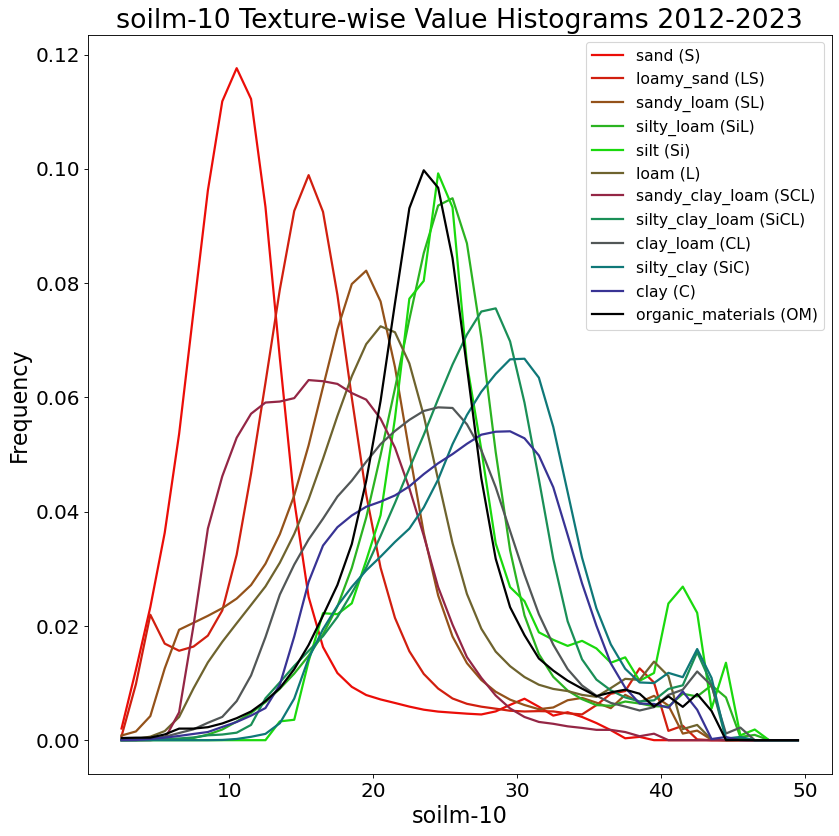
\includegraphics[width=.32\linewidth]{figures/thesis-gridstats/gridstat-hist-textures_soilm-10_2012-1_2023-12_y000-195_x000-462}
    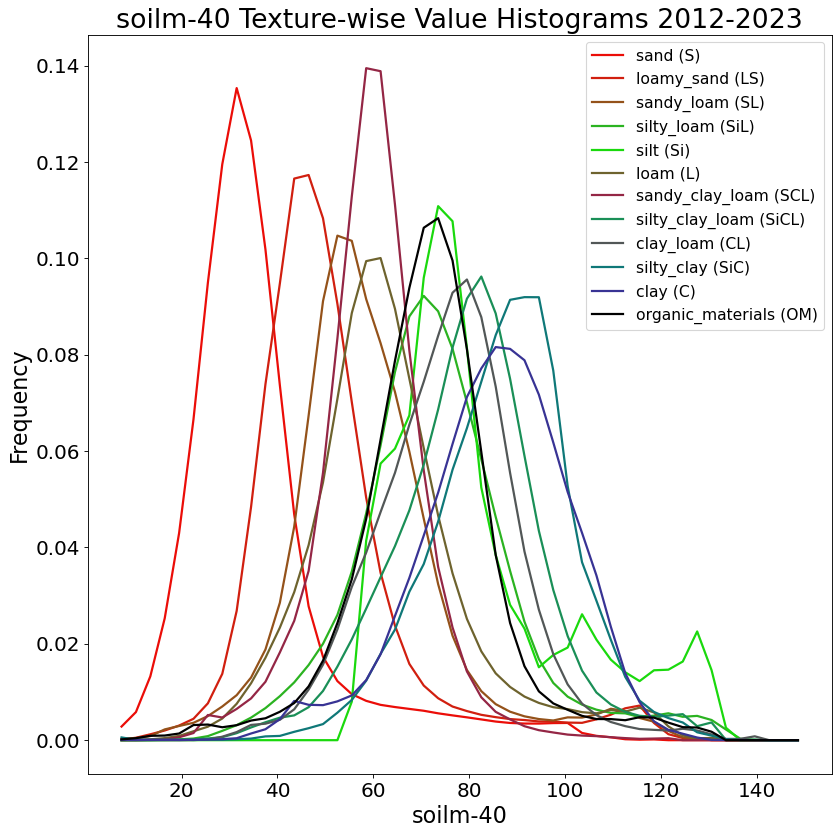
\includegraphics[width=.32\linewidth]{figures/thesis-gridstats/gridstat-hist-textures_soilm-40_2012-1_2023-12_y000-195_x000-462}
    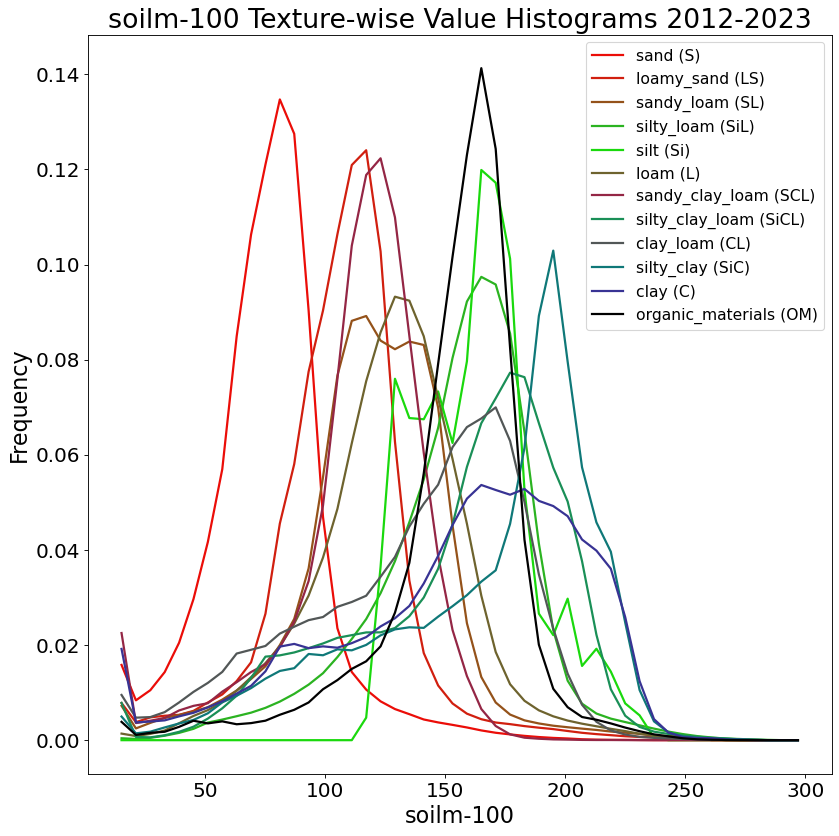
\includegraphics[width=.32\linewidth]{figures/thesis-gridstats/gridstat-hist-textures_soilm-100_2012-1_2023-12_y000-195_x000-462}

    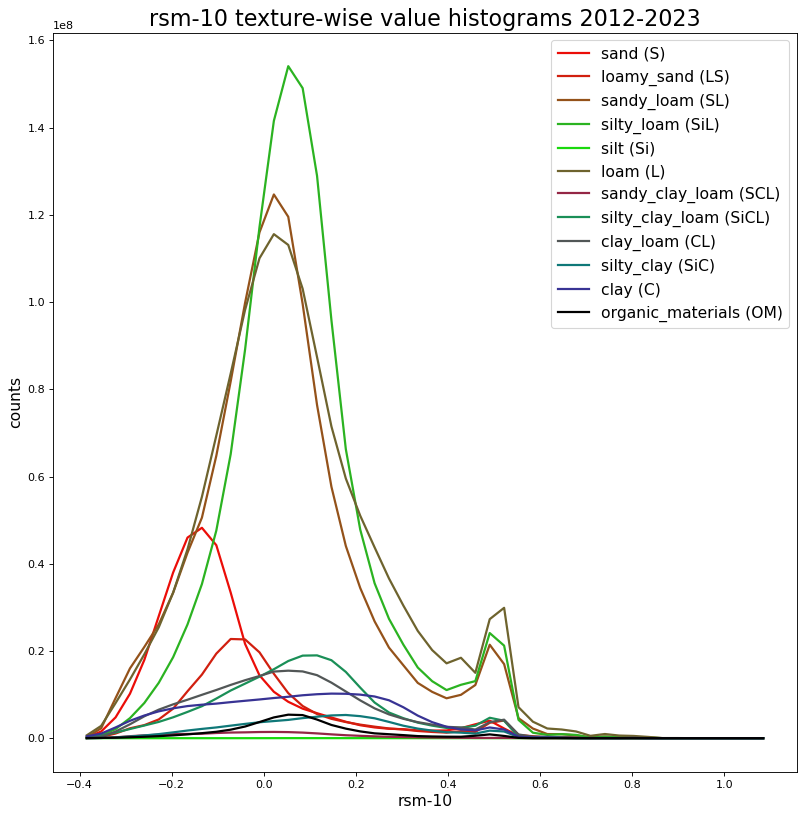
\includegraphics[width=.32\linewidth]{figures/thesis-gridstats/gridstat-hist-textures_rsm-10_2012-1_2023-12_y000-195_x000-462}
    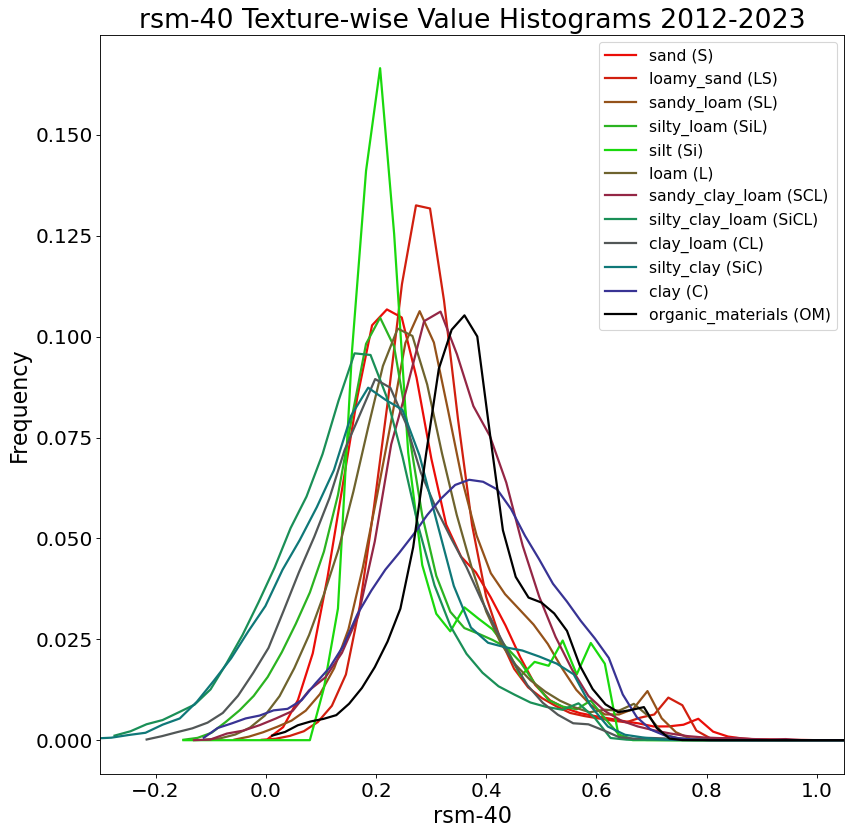
\includegraphics[width=.32\linewidth]{figures/thesis-gridstats/gridstat-hist-textures_rsm-40_2012-1_2023-12_y000-195_x000-462}
    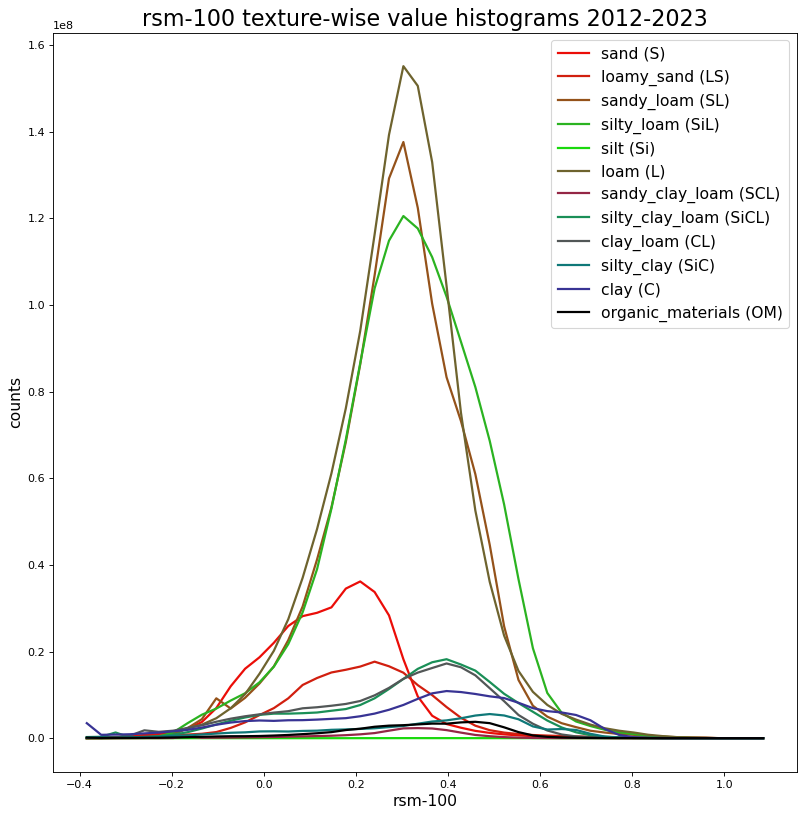
\includegraphics[width=.32\linewidth]{figures/thesis-gridstats/gridstat-hist-textures_rsm-100_2012-1_2023-12_y000-195_x000-462}


    \caption{Distributions of relative soil moisture (top) compared to those of soil moisture area density (bottom) at the first three depth levels, separated by soil texture category. Red, green, and blue components of line colors correspond to the sand, silt, and clay composition of the soil textures, respectively.}
    \label{dist-soilm}
\end{figure}

The differences in conductivity, matric potential, and other hydraulic properties among soil textures causes their distributions to occupy distinct value ranges, and their dynamics to vary at rates that are characteristic to each specific class. As the top row of Figure \ref{gs-rsm} indicates, the distributions of soil moisture area density (in $kg\,m^{-2}$) tends to stratify such that coarser textures (sandy blends) have generally lower moisture content per unit volume, and vice-versa with silt and clay dominant soil textures. Although there is some regional influence, this is mainly owed to the faster percolation rates and lower porosity of the coarser soil.

Since the loss function calculations are directly dependent on the magnitude of soil moisture, we hypothesized that significant differences in these value ranges could diminish the ANNs' ability to learn general solutions that apply to all soil textures. For example, since clay has a slow conductivity and infiltration rate and thus typically smaller magnitudes of increment change, loss calculations based on the increment change would be de-emphasized compared to sand. For this reason, we adopt the relative soil moisture as a physically-interpretable metric for normalizing soil textures to values that occupy roughly the same scale.

\begin{equation}\label{rsm-eq}
    \text{RSM} = \frac{\frac{\text{SOILM}}{d \, \rho_w} - \theta_{wp}}{\theta_s - \theta_{wp}}
\end{equation}

Relative soil moisture (RSM) linearly scales the water content such that each texture's wilting point is at zero, and saturation point corresponds to one. In Equation \ref{rsm-eq}, SOILM is the area density, $\rho_w$ is the density of water, $d$ is the depth of the soil layer, $\theta_s$ is the saturation point of a particular soil texture as a ratio of the total volume, and $\theta_{wp}$ is the wilting point. In this manner, the RSM can never exceed 1, but its lower bound is defined in terms of the hydraulic suction head needed to uptake further water. As such, very dry soils can have RSM values below zero. The layerwise comparisons of SOILM to RSM in Figure \ref{dist-soilm} make clear how RSM normalization aligns the individual texture distributions, and the added benefit of uniting the separate soil layers to a similar range of state values rather than using mass quantities that scale with their unique depths.

\begin{figure}[h!]
    \centering
    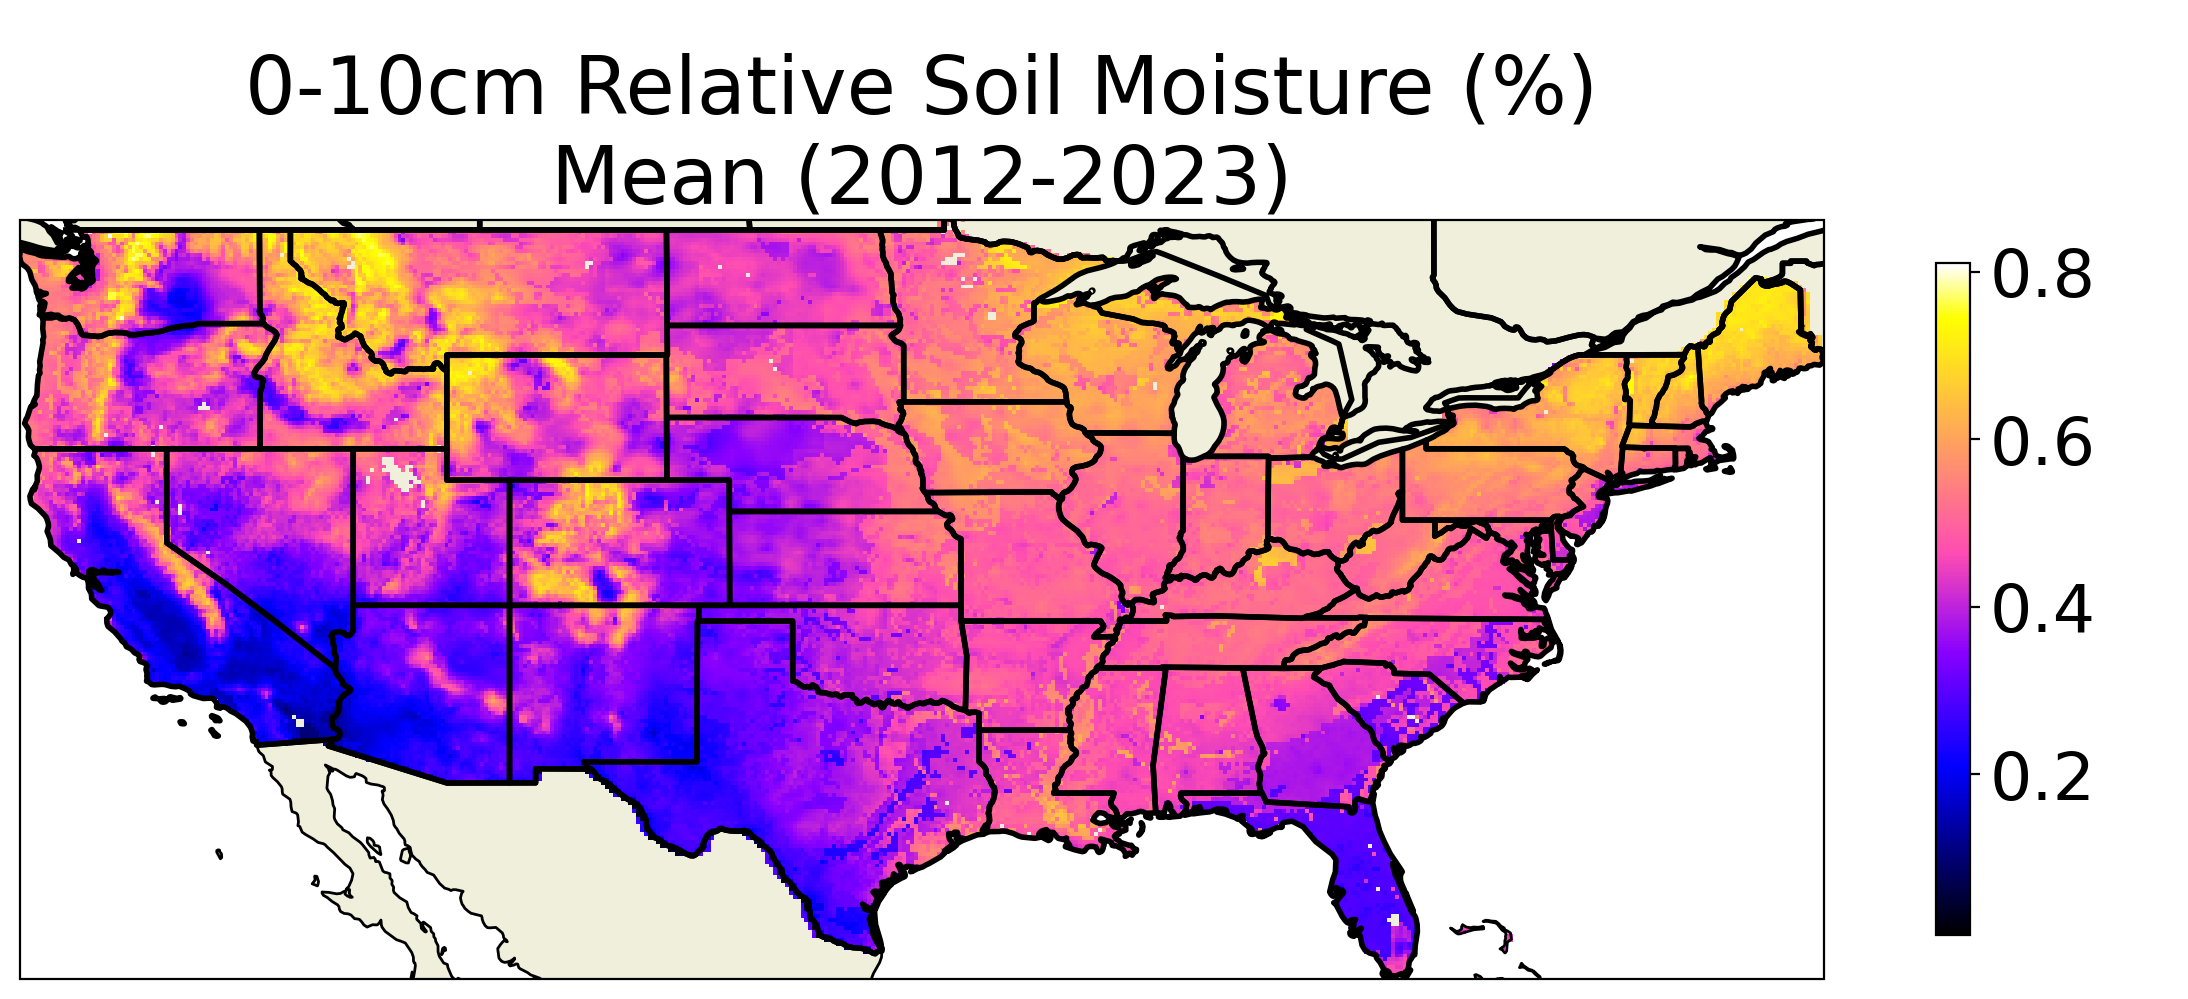
\includegraphics[width=.48\linewidth]{figures/thesis-gridstats/gridstat-bulk_rsm-10_2012-1_2023-12_y000-195_x000-462_mean.png}
    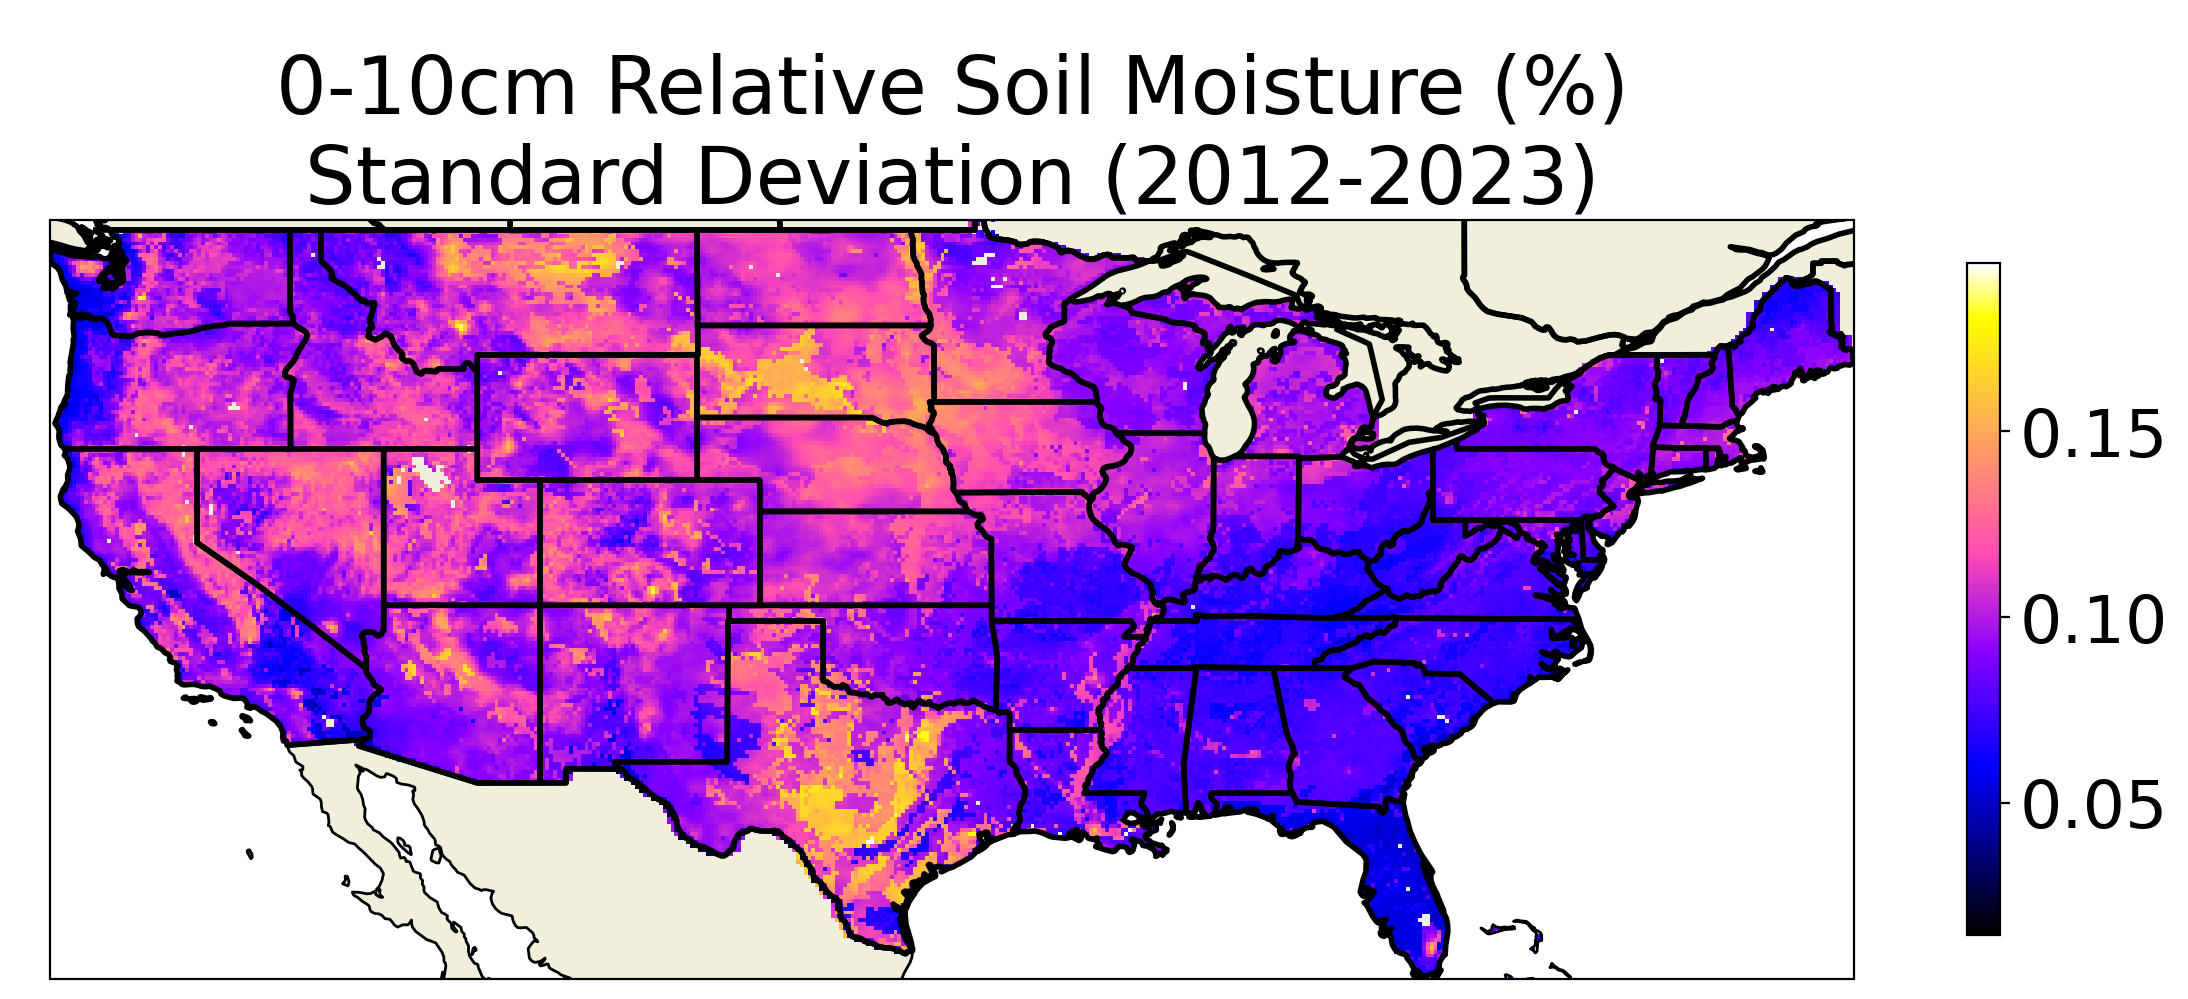
\includegraphics[width=.48\linewidth]{figures/thesis-gridstats/gridstat-bulk_rsm-10_2012-1_2023-12_y000-195_x000-462_stdev.png}
    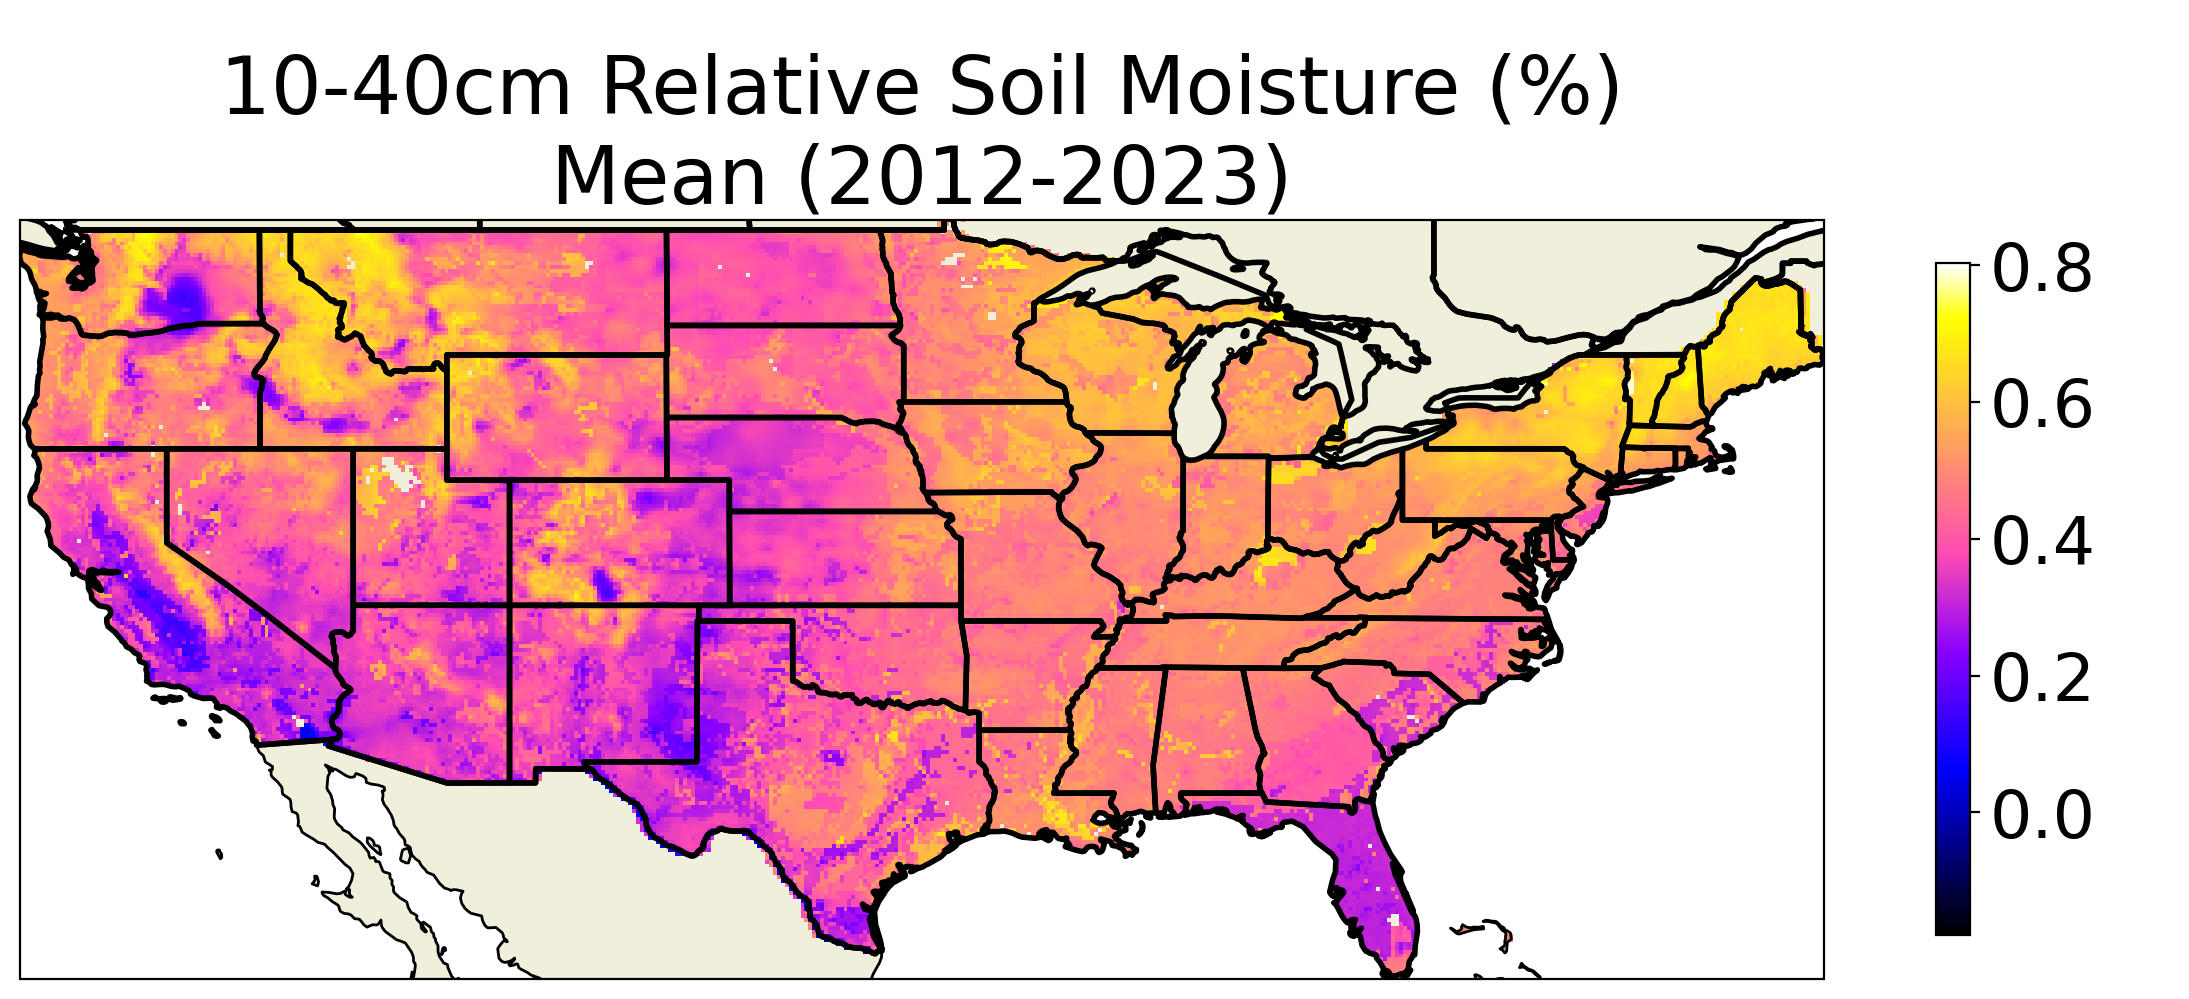
\includegraphics[width=.48\linewidth]{figures/thesis-gridstats/gridstat-bulk_rsm-40_2012-1_2023-12_y000-195_x000-462_mean.png}
    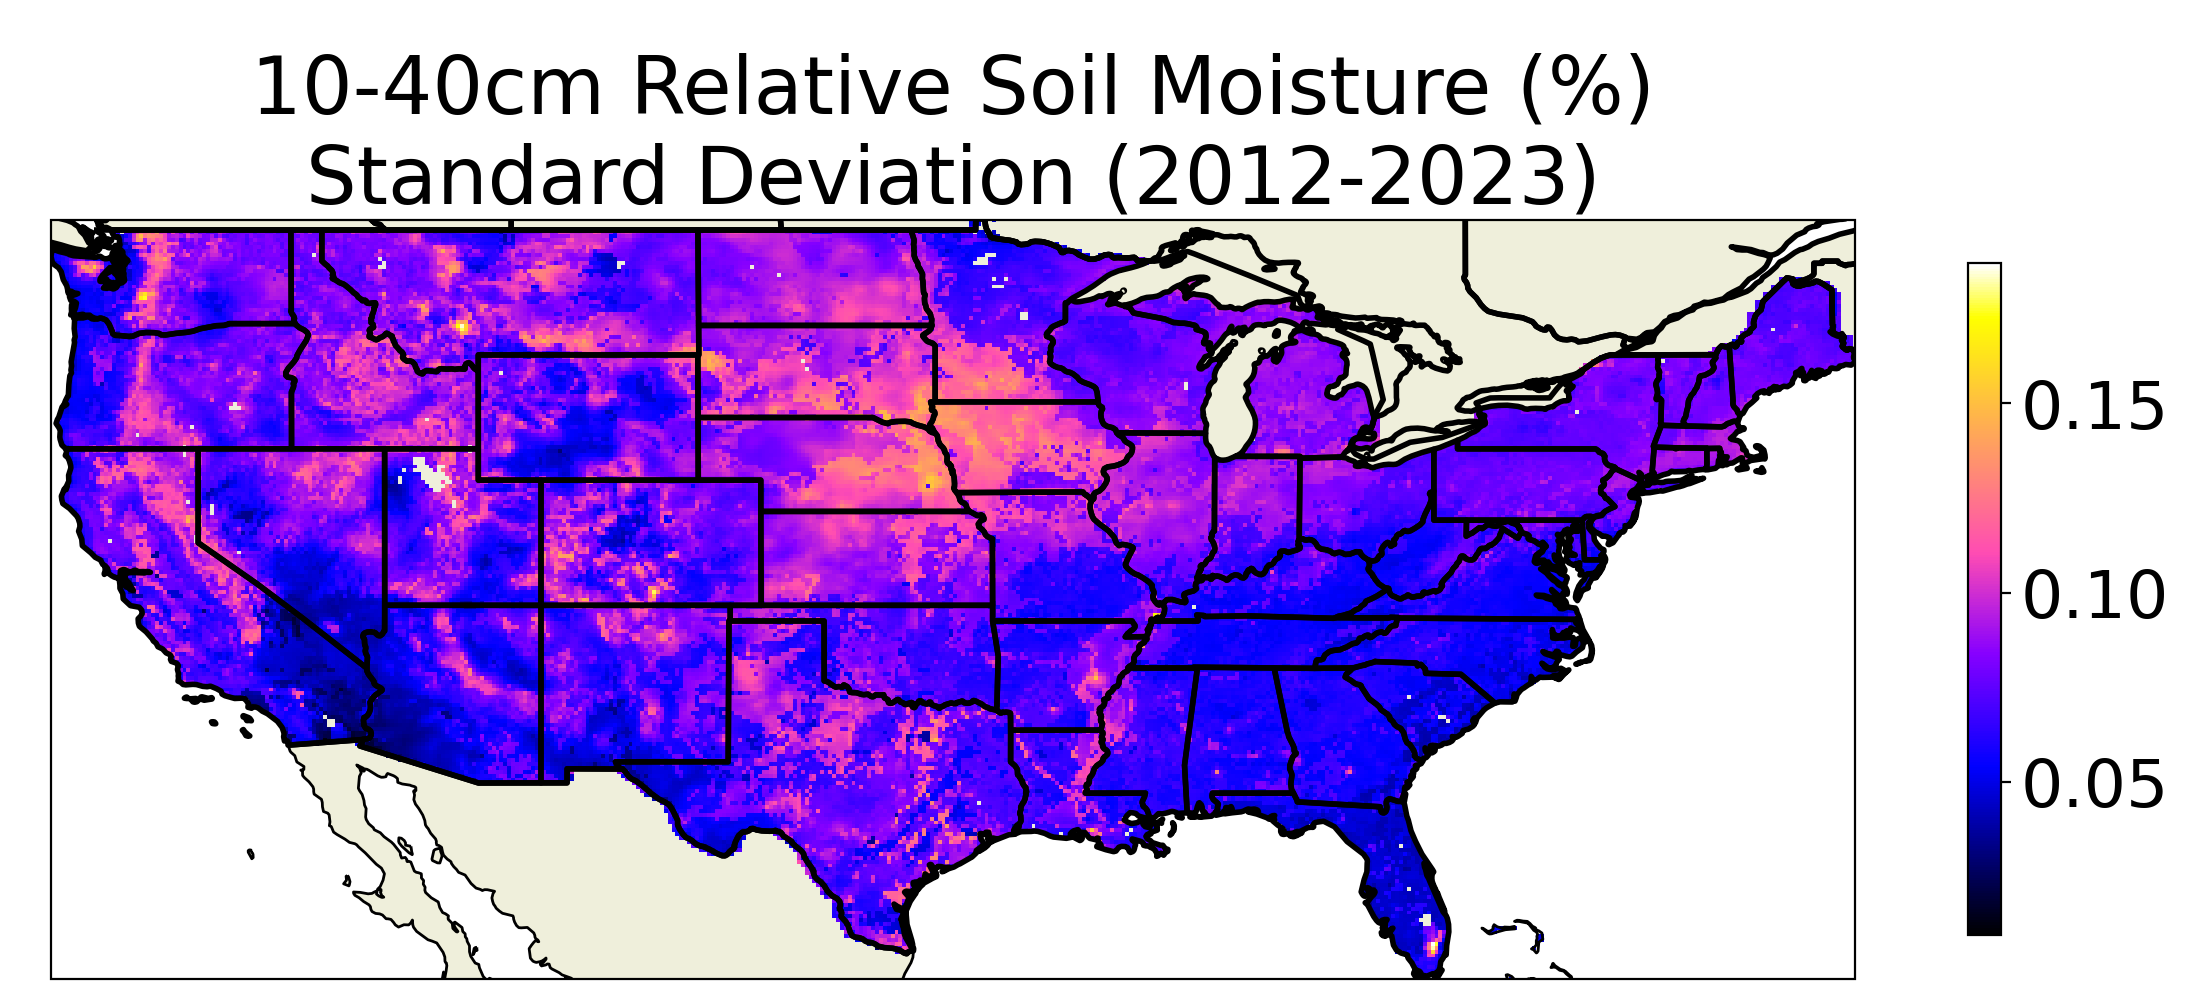
\includegraphics[width=.48\linewidth]{figures/thesis-gridstats/gridstat-bulk_rsm-40_2012-1_2023-12_y000-195_x000-462_stdev.png}
    \includegraphics[width=.48\linewidth]{figures/thesis-gridstats/gridstat-bulk_rsm-100_2012-1_2023-12_y000-195_x000-462_mean.png}
    \includegraphics[width=.48\linewidth]{figures/thesis-gridstats/gridstat-bulk_rsm-100_2012-1_2023-12_y000-195_x000-462_stdev.png}
    \caption{Gridded mean and standard deviation of relative soil moisture (2012-2023)}
    \label{gs-rsm}
\end{figure}

The spatial variation of soil moisture is depicted in Figure \ref{dist-soilm}, which emphasizes several important regional distinctions. The mountainous regions of the West remain rather saturated for much of the year -- especially in the upper soil layers -- owing to their high precipitation rates, the consistent presence of a snow pack, and limited drainage due to frozen soil. Sandy soils tend to have a lower average RSM than other soil types in a particular region due to their high hydraulic conductivity speedy drainage rates. The standard deviations were calculated using the overall per-pixel mean value; as such, clay-dominant soils generally have a higher standard deviation than other textures because their lower conductivity means they take more time to equilibrate after a rain event.

\section{Model Architectures}

The models that we tested fall into three broad architectural categories summarized in the background: fully-connected neural networks (FNNs), na\"ive RNNs, and LSTMs. In this subsection, we will elaborate on the particular implementation of these models for the unique problem structure of this project.

\begin{figure}[h!]
    \centering
    \includegraphics[width=.4\linewidth]{figures/schematic_accfnn.png}
    \caption{Schematic diagram of a multi-layered self-cycling fully connected neural network (FNN).}
    \label{accfnn}
\end{figure}

The basic fully-connected neural network variants we tested are structurally the most similar to Noah-LSM in the sense that the only information passed between time steps are the accumulated magnitudes of soil moisture at each layer given the prediction of the previous layer. As Figure \ref{accfnn} demonstrates, each timestep uses $L$ ANN layers \textbf{A$^(1)$}-\textbf{A$^(L)$} to transform the previous state, current forcing, and static parameter inputs into a prediction for the increment change in state. Only one initial state value $\vec{s}_{-1}$ is needed to run the model since it doesn't require a multi-step initialization window. The most performant instance of this architecture will serve as a good baseline for understanding the benefit of introducing more structural complexity in the subsequent model types.

\begin{figure}[h!]
    \centering
    \includegraphics[width=.95\linewidth]{figures/schematic_s2s-embed.png}

    \caption{Sequence-to-sequence RNN architecture with initial projection layers \textbf{M}, spin-up window cells \textbf{G} for initializing first-step weights, prediction horizon cells \textbf{E}, and fully-connected decoder layer \textbf{D}.}
    \label{s2s-default}
\end{figure}

The na\"ive RNN and LSTM are distinct from the FNN in that they provide a hidden vector based on past timesteps to supplement the input at each subsequent timestep. In order to initialize the hidden vectors provided to first prediction timestep ($\vec{h}^{(l)}_{init}$ for $l \in [1,\,L]$) with values providing context about the recent history of soil states, we add a spin-up window (\textbf{G}$^{(l)}$) that observes the $W$ timesteps prior to the first prediction and produces a vector for each layer of the output sequence. This principle is diagrammed in Figure \ref{s2s-default}, and applies to both the na\"ive RNN and LSTM. In contrast to the prediction horizon sequence, the spin-up window explicitly receives surface states as inputs, and hidden states of each layer at the final timestep are the only values captured and passed along. For both of these reasons, the spin-up window sequence's weights are not shared with the forecast horizon sequence.

The next architecture we explored was the na\"ive RNN, which has multiple layers of cells that each produce an output based on 3 sets of weights applied to a latent vector from the previous timestep and an input vector from the layer below. The LSTM is similar except that each cell contains 4 sets of weights with outputs that are algebraically combined to produce the output rather than operated upon by a matrix transformation. For further details, refer back to Figure \ref{rnns-both} and Equation \ref{eq_rnn}.

\begin{figure}[h!]
    \centering
    \includegraphics[width=.95\linewidth]{figures/schematic_s2s-accumulator-embed.png}

    \caption{Sequence-to-sequence RNN with explicit output state accumulation.}
    \label{s2s-accumulator}
\end{figure}

When the inference algorithm is executed for a multi-layer RNN, every timestep of each layer is evaluated before the hidden states are passed along to a higher-level layer; there is no mechanic for information from the higher layers of previous timesteps to be passed along to the lower layers of subsequent steps. In contrast, the governing equations of Noah-LSM -- including the Richardson equation, plant parameterization, and bare-surface evaporation -- depend very strongly on the magnitude of soil moisture present at any given timestep. As such, we hypothesized that providing an explicit estimate of the soil moisture state as an input at each step would improve prediction skill. As Figure \ref{s2s-accumulator} demonstrates, we implemented this by encapsulating all the layers as a single RNN cell and adding the predicted increment change to the previous state after each step. We will refer to na\"ive RNN and LSTM variants employing this strategy as ``accumulators'', abbreviated as AccRNN and AccLSTM.

All of the models presented here will predict the increment change in state rather than the state magnitude, consistent with the numerical model's estimation of the time derivative as in Equation \ref{dynamical}. Early exploratory testing revealed that models which directly predict the soil state produced very erratic and physically unreasonable results, while predicting increment change led to smoother and more responsive estimates. We suspect that this is because the change in state correlates far more strongly with the current atmospheric forcings than the state magnitude, as many different environmental circumstances could lead to a particular soil state magnitude, but conditions like precipitation, humidity, and temperature have a direct influence on the immediate change in state.

Notice that unlike the numerical model described by Equation \ref{dynamical}, which contains a variable increment change in time $\Delta t$, none of the neural network architectures here have a facility for determining the temporal resolution of predictions they generate. Instead, the coarseness of the timestep is implicit based on the training data, and cannot be changed after training; as such, the coarseness is an independent variable of the training configuration. Unless otherwise specified, the models presented here are all trained at the native 1 hour resolution of the forcing dataset (although the computational timestep of Noah-LSM is 15 minutes), however some models trained at 3 hour or 6 hour resolution showed very promising results. A more thorough analysis of the effect of courser time resolutions on prediction accuracy and model efficiency is left for future work.

\section{Training Paradigm}

One of the main challenges of developing ANNs is contending with the overwhelming number of parameters that can influence model behavior. The modeler must decide on a learning rate schedule, loss function characteristics, the number of layers within the model, the number of trainable weights within each layer, and many other parameters for which there are few reliable standards or heuristics that apply generally to different problem types. To address this, we initially trained 10-25 ANNs within each category while varying multiple parameters between generations based on intuition, and in order to capture a wide breadth of configurations. After these exploratory training runs, we selected the best models from each category and re-trained them while only perturbing one parameter at a time in both directions. For instance, increasing and decreasing the number of layers by one. Finally, the models in each architectural category having the best bulk statistical performance were selected for further more detailed evaluation.

All of the model training was executed on a CPU cluster with 32 cores, and training was allowed to proceed until the prediction skill stopped increasing for a validation dataset (withheld from training) for 48 epochs. In this context, the epoch refers to the number of updates to the model weights between performance reports, which we set to 256. In this environment, training would usually conclude in less than 36 hours. In order to logistically facilitate working with this large number of models, we developed a simple but robust system for storing, deploying, and provisioning data for models based on a set of rigorous configuration standards.

We use functional generators to load, scale, and restructure data on-demand from the source \texttt{timegrid} files during training. This involves extracting sparsely-sampled chunks from multiple files, separating the data into arrays for the spin-up window, prediction horizon inputs, target values, and static data ordered as a set of uniform-length sequences, and linearly normalizing data values so that they approximate a unit gaussian. As mentioned in the beginning of this chapter, it is important to globally shuffle the data used for training in order to avoid over-fitting to a data distribution that only describes a subset of the full domain, so the sequence samples from separate chunks are randomly interleaved. The data generators also accommodate ``derived'' features that are calculated on-demand as a function of the stored features rather than being stored in parallel, which enables target values like RSM or inputs like wind magnitude and relative humidity to be used during training and evaluation without occupying extra disc space and forcing costly re-generation of the \texttt{timegrid} files.

\begin{figure}[h!]
    \centering
    \includegraphics[width=.48\linewidth]{figures/cyclical_lr_logarithmic.png}
    \includegraphics[width=.48\linewidth]{figures/learning-curves_acclstm.png}

    \caption{Learning rate schedule and subsequent learning curves for AccLSTM architectures.}
    \label{learning-rate}
\end{figure}

One of the most important considerations for ANN training setup is the learning rate schedule, which governs the sensitivity of the model's trainable weights to the prediction cost given new data during training. If the learning rate is too high, training may not converge on an optimal solution that relies on fine-grained changes in weights, while if the learning rate is too low, the learning process may take too much time, and could prematurely halt after getting stuck in a local minimum of the loss environment which would require a larger update in model weights to resolve \citep{russell_artificial_2020}. Practitioners generally start with a high learning rate early in training, and schedule it to gradually decrease as training proceeds \citep{ren_understanding_2024}, however a separate promising strategy is to cycle between lower and higher learning rates many times \citep{smith_cyclical_2017}. We mainly utilized a combination of these two methods as shown in the left panel of Figure \ref{learning-rate}, which introduces new tunable parameters including the period of cycles, magnitude of decay, and initial minimum and maximum learning rate.

The loss function is even more critical in determining how the model ultimately behaves, given that it defines the standard for quantifying the skill of predictions. Many applications will simply employ mean absolute error (MAE) or mean squared error (MSE) as the loss metric without further changes, however as long as the functions remains differentiable, modifications can emphasize or de-emphasize certain outputs, balance multiple goals, or assign importance to individual samples based on properties of their data. As such, we tested the effects of manipulating three characteristics of the loss function. First, the values normalized to a unit gaussian in the data generator include the inputs and the target soil moisture state magnitude, however the increment change in soil moisture has its own characteristic distribution that is unique to each soil layer. To address this, we implemented an optional second normalization of increment change values that is only applied within the loss function. In effect, this serves as a coefficient that scales the ratio of the loss associated with each of the output values. Second, the models should prioritize making the locally optimal prediction at each timestep, but they should also be incentivized to recover from error in previous step predictions and produce the globally optimal sequence. To incorporate both of these goals, we introduced a tunable ratio that combines the step-wise error with the integrated state error at each time step. Finally, accurate predictions at some timesteps is considerably more important for producing skillful sequences than many others. For example, a summertime thunderstorm that produces 12cm of precipitation in an hour followed by a two hour surface runoff event will often have a larger influence on the soil column than a subsequent week of drydown near equilibrium. The loss contribution of circumstances like these can be emphasized by adding an additional cost proportional to the true magnitude of change in each layer.

\begin{equation}\label{loss-fn}
    \begin{split}
        L(X',\,Y) &= \rho\,P(X',\text{diff}(Y)) + (1-\rho)\,Q(\text{acc}(X')+Y_{j=0},Y) \\
        P(X',\,Y') &= \frac{1}{S}\,\sum_{i=0}^N \sum_{j=0}^S (1+\gamma \left|Y'_{i,j}\right|)\,\frac{\left|X'_{i,j}-Y'_{i,j}\right|}{\lambda_i} \\
        Q(X,\,Y) &= \frac{1}{S}\,\sum_{i=0}^N \sum_{j=0}^S \left|X_{i,j}-Y_{i,j+1}\right| \\
    \end{split}
\end{equation}


Equation \ref{loss-fn} formalizes the loss function definition for a single pair of prediction ($X$) and target ($Y$) values with $N$ output values (soil layers) and $S$ sequence steps. The arguments to the top-level function $L$ are the $N$ predicted increment changes $X'$, and the $L+1$ true state values (which includes the land surface state immediately prior to the first prediction step). The ``diff'' function is the discrete forward difference along the sequence axis converting the true states to the true increment changes, and the ``acc'' function is the cumulative sum of the predicted changes along the sequence axis. Then $P(X',Y')$ handles the loss contribution of the increment changes, and $Q(X,Y)$ represents that of the state magnitude, which are balanced by the increment loss ratio $\rho$. The $\lambda_i$ parameter serves as the pre-determined normalization coefficient for soil layer $i$, and the magnitude bias parameter $\gamma$ scales the sensitivity of the loss in proportion with the absolute value of the increment change.

\section{Evaluation Metrics}

\begin{equation}
    \label{metric_pcc}
    r(x,y) = \frac{\sum_{i=0}^{N}(x_i-\bar{x})\,(y_i - \bar{y})}{\sqrt{\sum_{i=0}^N(x_i - \bar{x})^2} \cdot \sqrt{\sum_{i=0}^N(y_i-\bar{y})^2}}
\end{equation}

\begin{equation}
    \label{metric_mae}
    MAE(x,y) = \frac{1}{N}\sum_{i=0}^{N}\left|y_i-x_i\right|
\end{equation}

\begin{equation}
    \label{metric_rmse}
    RMSE(x,y) = \sqrt{\frac{1}{N}\sum_{i=0}^{N}\left(y_i-x_i\right)^2}
\end{equation}

The metrics we will use to evaluate the ANN's performance include the pearson correlation coefficient, mean absolute and mean squared error, error bias, as well as entropy-based metrics including information loss and fractional information. The pearson coefficient measures the strength and direction of the linear relationship between variables in terms of the ratio between their covariance and the product of their individual standard deviations. In this case, the variables compared are the target and predicted soil moisture content or the hourly increment change in soil moisture content. A value of 1 would indicate a perfect positive linear relationship, while zero suggests no correlation, and -1 a perfect inverse linear correlation. We calculate the pearson coefficient in accordance with Equation \ref{metric_pcc} independently for each 2-week prediction sequence, then average the results across pixels and initialization times to get the values presented in the following chapter.

Unlike the pearson coefficient, which is scale-invariant, the mean absolute and root mean squared error (MAE, RMSE) metrics present results using the same units as the subject data. MAE is straightforwardly the expected error for a randomly selected target and prediction data pair (Equation \ref{metric_mae}), while RMSE utilizes the average squared difference in data pairs, which makes the metric more sensitive to high-error outliers (Equation \ref{metric_rmse}). Since both of these metrics are differentiable, they can both be used as loss functions while training ANNs. In Equation \ref{loss-fn} -- and by default for most of the models presented here -- we used MAE as the essential form of the loss function, however we will test models trained to optimize the squared error as well.

\begin{figure}[h!]
    \centering
    \includegraphics[width=.54\linewidth,draft=false]{figures/entropy.png}
    \includegraphics[width=.44\linewidth,draft=false]{figures/validation-curves/eval_test_lstm-rsm-9_rsm-10_hist-true-pred_na.png}

    \caption{Entropy curve for a single possible state of a system with respect to the probability of that state being occupied, and an example of a joint histogram validation curve from which the total entropy is calculated.}
    \label{entropy}
\end{figure}

The metrics above all in some way characterize the deviation of the data pairs from a linear relationship. These are straightforward to calculate and especially meaningful for relatively small amounts of data, however for large volumes of data the error rates under the most common conditions can overshadow important characteristics of model behavior in edge cases. As such, when we are considering a large enough volume of data to sufficiently approximate the true distribution of data values, we will also evaluate the ANNs in terms of the uncertainty contribution (also known as information loss) and fractional information according to the methodology used by \citep{nearing_benchmarking_2016} to the benchmark the uncertainty of Noah-LSM in terms of contributions from the input forcings, model parameters, and model structure. Unlike the correlation coefficient, MAE, and MSE, the fractional information and uncertainty contribution are used to characterize the extent to which using the ANN rather than the source model introduces ambiguity in the distribution of hourly change in RSM by creating a sub-distribution of predictions corresponding to each target. These metrics operate on global properties of the distribution of evaluation results that are less vulnerable to imbalances in the data.

\begin{equation}\label{eq-entropy-h}
    H(z) = - \sum_{i=1}^B \frac{n^{(z)}_i}{N}\ln\left(\frac{n^{(z)}_i}{N}\right) % entropy
\end{equation}

\begin{equation}\label{eq-entropy-i}
    I(y^A,\,y^M) = H(y^M) + H(y^A) - H((y^A,\,y^M)) % mutual information
\end{equation}

The following discussion of the principles and mathematical formalisms from information theory are based on Chapter 2 of Elements of Information Theory \citep{schilling_entropy_2005}. The information metrics we will use are functions of the Shannon entropy $H(z)$ of the distributions of increment change in RSM, and are estimated in terms of the discrete joint histograms of the targeted and predicted values, such as the one pictured on the right of Figure \ref{entropy}. In Equation \ref{eq-entropy-h}, $n^{(z)}$ represents a histogram of arbitrary variable $z$ with $B$ bins, which counts the integer number of occurrences of data within the value range described by each bin. Each of the bin counts are divided by the total number of observations $N$ to yield the probability of a randomly selected sample occupying that position within the histogram. The integrand function plotted on the left-hand side of Figure \ref{entropy} is applied to the probability associated with each of the bins in order to calculate their individual information contribution to the system, and the total entropy of the distribution is estimated as the sum of the contributions of the bins.

To better understand the properties of a distribution that entropy characterizes, consider a hypothetical distribution that describes a system with a large number of low or zero-probability configurations, and a small number of high-probability configurations. As Figure \ref{entropy} suggests, both the low and high-probability configurations correspond to a relatively small entropy contribution. In contrast, a different hypothetical distribution having probabilities that are spread uniformly across its possible configurations will have a relatively large entropy contribution from each of them, so the sum total entropy of the latter distribution will be higher than the former. In this sense, as described by \citep{schilling_entropy_2005}: ``the entropy of a random variable is a measure of the uncertainty of the random variable; it is a measure of the amount of information required on the average to describe the random variable''.

Entropy is a fundamental property of a distribution with units of information depending on the base of the logarithmic function used to calculate the integrand. In our case, we use the natural logarithm, which corresponds to ``natural units'' or nats. One of the main advantages of entropy is its chain rule property, which facilitates an additive relationship between the entropy of independent variables and that of their joint distribution. As a consequence, we can straightforwardly calculate the mutual information $I(y^A,\,y^M)$ of two variables, which is a commutative metric of the reduction in uncertainty of one given knowledge of the other. In Equation \ref{eq-entropy-i}, $y^A$ refers to the histogram of increment RSM values predicted by the ANN, $y^M$ to the histogram of Noah-LSM values, and $(y^A,\,y^M)$ to their joint histogram.

\begin{equation}\label{eq-entropy-fi}
    FI(y^A,\,y^M) = \frac{I(y^A,\,y^M)}{H((y^A,\,y^M))} % Fractional Information
\end{equation}

\begin{equation}\label{eq-entropy-u}
    U(y^A;\,y^M) = H(y^A) - I(y^A,\,y^M) % Uncertainty contribution of ANN
\end{equation}

In practice, we will use the entropy and mutual information values to calculate the derived metrics of fractional information ($FI(y^A,\,y^M)$, Equation \ref{eq-entropy-fi}) and uncertainty contribution ($U(y^A;\,y^M)$, Equation \ref{eq-entropy-u}) to characterize the efficiency of the ANNs at emulating the information characteristics of Noah-LSM. Fractional information normalizes the mutual information by the total entropy of the joint distribution, which returns a more familiar ratio value since $H((y^A,\,y^M))$ is a strict upper bound on mutual information. The uncertainty contribution (or information loss) remains in the unit of nats, and explicitly articulates the additional entropy (that is, uncertainty) supplied by employing the ANN rather than the source model.
